\documentclass[10pt, a4paper]{book}

\usepackage{verbatim}
\begin{comment}

    书名: C语言入门指南
    作者: 吴同
    编码: UTF-8

    \end{comment}

\label{导言区}

\usepackage[heading=true]{ctex}
\usepackage{commath}
\usepackage{graphicx}
\usepackage{float}
\usepackage{caption}
\usepackage{bookmark}
\usepackage{booktabs}
\usepackage{amssymb}
\usepackage{verbatim}
\usepackage{framed}
\usepackage{mdframed}
\usepackage{enumitem}
\usepackage{threeparttable}
\usepackage[perpage]{footmisc}
\usepackage{blindtext}
\usepackage{longtable}
\usepackage{multirow}
\usepackage{booktabs}
\usepackage{wallpaper}

\usepackage{amsmath}
\allowdisplaybreaks

\usepackage{color}
\usepackage{xcolor}
\definecolor{linenumbercolor}{RGB}{128,138,135}     % 代码环境行号数字颜色
\definecolor{keywordcolor}{RGB}{3,95,205}           % 代码环境关键字颜色
\definecolor{commentcolor}{RGB}{34,139,34}          % 代码环境注释颜色
\definecolor{stringcolor}{RGB}{128,0,0}             % 代码环境字符串颜色
\definecolor{backgroundcolor}{RGB}{245,245,244}     % 代码背景颜色

\usepackage{hyperref}
\hypersetup{
    pdfpagelayout=TwoColumnLeft,
    colorlinks=true,
    linkcolor=blue,
    filecolor=blue,      
    urlcolor=blue,
}

\mdfsetup{
    linecolor=darkgray,
}

\usepackage{geometry}
\geometry{inner=3.5cm, outer=2.5cm, top=3.5cm, bottom=3.5cm}
\setlength{\headheight}{15pt}

\usepackage{setspace}
\onehalfspacing
\addtolength{\parskip}{1em}

\usepackage{titlesec}   % 这段代码能够修改前言, 说明和后记的章节标题样式, 原理未知, 为什么不修改正文章节标题未知.
\makeatletter
\renewcommand{\@makeschapterhead}[1]{%
  \vspace*{20\p@}%
  {\parindent \z@
    \normalfont
    \interlinepenalty\@M
    \Huge \bfseries  #1\par\nobreak
    \vskip 20\p@
  }}
\makeatother

\ctexset{
    chapter={
        name={第,章},
        format+=\heiti
        
    },
    section={
        format+={\raggedright\Large\heiti}
    },
}

\usepackage{fancyhdr}
\pagestyle{fancy}
\fancyhf{}
\fancyhead[LO]{\bfseries\leftmark}
\fancyhead[RE]{\bfseries\rightmark}
\fancyfoot[LO,RE]{\bfseries\thepage}
\renewcommand{\headrulewidth}{0.5pt}
\renewcommand{\footrulewidth}{0pt}
\addtolength{\headheight}{0.5pt}
\fancypagestyle{plain}{
  \pagestyle{fancy}
}

\usepackage{afterpage}
\newcommand\emptypage{
    \null
    \thispagestyle{empty}
    \addtocounter{page}{-1}
    \newpage
}

\usepackage{listings}
\lstset{
    escapeinside=@@,                                        %  逃逸字符
    numbers=left,                                           %  在左侧显示行号
    numberstyle=\color[RGB]{128,138,135},                   %  设置行号格式
    basicstyle=\footnotesize,                               %  设置代码字号.
    basicstyle=\tt,                                         %  设置代码字体
    breaklines=true,                                        %  设置自动断行.
    extendedchars=true,                                     %  是否允许使用非ASCII字符; 仅适用于8位编码,不适用于UTF-8.
    extendedchars=false,                                    %  解决代码跨页时,章节标题,页眉等汉字不显示的问题
    xleftmargin=2em,xrightmargin=2em, aboveskip=1em,        %  设置边距
    tabsize=4,                                              %  设置tab空格数
    showspaces=false                                        %  不显示空格
    frame=none,                                             %  不显示背景边框
    backgroundcolor=\color[RGB]{245,245,244},               %  设定背景颜色
    keywordstyle=\color[RGB]{3,95,205},                     %  设定关键字颜色
    commentstyle=\tt\color[RGB]{34,139,34},                 %  设置代码注释的格式
    stringstyle=\color[RGB]{128,0,0},                       %  设置字符串格式
    showstringspaces=false,                                 %  不显示字符串中的空格
    language=c++,                                           %  设置语言
    morekeywords={alignas,continute,friend,register,true,alignof,decltype,goto,reinterpret_cast,try,asm,defult,if,return,typedef,auto,delete,inline,short,typeid,bool,do,int,signed,typename,break,double,long,sizeof,union,case,dynamic_cast,mutable,static,unsigned,catch,else,namespace,static_assert,using,char,enum,nestatic_cast,virtual,char16_t,char32_t,explict,noexcept,struct,void,export,nullptr,switch,volatile,class,extern,operator,template,wchar_t,const,false,private,this,while,constexpr,float,protected,thread_local,const_cast,for,public,throw,std},
}

\renewcommand{\lstlistingname}{代码片段}
\renewcommand{\lstlistlistingname}{代码片段}

\newcommand{\sla}{\texttt{\textbackslash}}


\begin{document}

    \frontmatter

    \label{前封面}
\ThisCenterWallPaper{1}{pic/cover/frontcover.png}
\pagecolor{cover_background_white}
\emptypage 
\pagecolor{white}
\emptypage

\label{扉页}
\ThisCenterWallPaper{1}{pic/cover/flypage.png}
\emptypage \emptypage

    \setcounter{tocdepth}{1}
    \tableofcontents

    \chapter*{前言}
\addcontentsline{toc}{chapter}{前言} \label{前言}
\fancyhead[LO,RE]{\bfseries 前言}

    C语言(在不引起歧义的情况下简称C)以简洁优雅著称, 语法简练, 功能强大; 同时又是最早被广泛使用的高级语言, 可以毫不夸张地说, 计算机世界的地基是C语言一行行写出来的. 学习C语言, 不仅能一定程度上帮助解决日常学习工作中遇到的问题, 更重要的是能够一窥计算机的底层运行方式, 并为将来学习其它计算机领域打下稳固的基础.

    这是一份C语言入门指南. 旨在帮助没有任何基础的新手入门C语言.

    \leavevmode \\
    指南中你将学到:
    \begin{itemize}
        \item 有关编程语言和计算机技术的基础知识.
        \item 如何使用C语言编写程序并运行.
        \item 如何规范地组织代码.
        \item 一些利用代码解决问题的编程思维.
    \end{itemize}

    \noindent
    你将不会学到:
    \begin{itemize}
        \item 复杂算法, 数据结构等非语法内容.
        \item 多文件编程, 项目管理等工程代码内容.
    \end{itemize}

    \noindent
    指南受众:
    \begin{itemize}
        \item 有一定的数学基础.
        \item 对编程有兴趣.
        \item 不需要对编程有提前了解.
    \end{itemize}

    \vspace*{5pt}

    欢迎来到编程的世界.

\chapter*{说明}
\addcontentsline{toc}{chapter}{说明} \label{说明}
\fancyhead[LO,RE]{\bfseries 说明}

    指南中小节标题形如 \texttt{*}标题\texttt{*} 的表示该部分内容为较复杂或较不常用的内容, 对完成简单的程序无较大影响, 初次阅读可跳过, 这些章节也不会赘述过多细节. 这些小节被放在章的末尾.

    \vspace*{5pt}
    指南中形如这样地内容表示正文. 

    \vspace*{5pt}
    指南中形如\textbf{这样的内容}表示我对读者的建议.

    \begin{itemize}
        \item 指南中形如这样的内容表示准则.
    \end{itemize}

    \begin{description}
        \item[对象] 指南中形如这样的内容表示对对象的说明. 
    \end{description}

    \vspace*{-20pt}
        \[ \mbox{指南中形如这样的内容表示强调的式子.} \]

\begin{lstlisting}
//指南中形如这样的内容表示代码.
\end{lstlisting}

\lstset{
    numbers=none,
    keywordstyle=\color[RGB]{255,255,255},
    commentstyle=\color[RGB]{255,255,255},
    stringstyle=\color[RGB]{255,255,255}
}
\begin{lstlisting}
指南中形如这样的内容表示程序输入, 输出和信息. 指南中不会列出所有代码的输出, 读者可以自行实验.
\end{lstlisting}
\lstset{
    numbers=left,
    keywordstyle=\color[RGB]{3,95,205},    
    commentstyle=\color[RGB]{34,139,34},   
    stringstyle=\color[RGB]{128,0,0}
}

    \vspace*{5pt}
    指南中\href{https://www.baidu.com}{形如这样的内容}表示链接, 可以点击跳转到对应的图, 表, 网页, 注释或章节. 手机端可能无法使用此功能.

    \begin{mdframed}[linecolor=darkgray]
        代码中形如这样的内容表示涉及到 \texttt{*}章节\texttt{*} 内容的文本.
    \end{mdframed}

    指南中部分内容为了方便初学者理解, 在不损失主干逻辑的前提下做了简化, 一般会用括号标注, 或在脚注中补充详细内容. 同时我们也鼓励读者自行上网搜索. 我们也将在第\ref{错误和警告}节中提到搜索信息的技巧.

    指南中难免有疏漏之处, 敬请读者谅解. 如遇错漏, 望能告知: \href{mailto: wutong.tony@foxmail.com}{我的邮箱}.

    另外, 请不要阅读国内某些编程出版物. 它们是邪恶的, 错误的, 恼人的, 里面包含了大量原则性错误, 只会误导新手. 建立一个正确的编程规范是非常重要的.

    \mainmatter

    \chapter{编程基础} \label{编程基础}
\fancyhead[LO]{\bfseries\leftmark}
\fancyhead[RE]{\bfseries\rightmark}
    \section{编程语言和C语言简介}
        计算机的核心运算单元是CPU, 但是CPU只能读取并执行由01串写成的命令(称为机器码). 例如 $ 01010111 \ 00101100 \ 01001001$ 可能表示将地址为 $ 00101100 $ 和 $ 01001001 $ 的数据加起来, 再将结果写回 $ 00101100 $ 中. 不难看出, 这样的代码晦涩难懂, 很难理清逻辑, 并且容易拼写错误导致BUG.

        所以汇编出现了. 汇编是一种低级语言(低级语言和高级语言只是一种分类, 没有感情色彩), 它给每个机器码起了个名字称为助记符, 又可以反过来将一系列助记符编译成机器码, 二者一一对应. 例如前面提到的例子中, 我们把加命令 $ 01010111 $ 写作ADD, 把地址 $ 00101100 \ 01001001 $ 分别起个名字叫eax和ebx, 于是就有了对应的汇编代码
\begin{lstlisting}
ADD eax,ebx
\end{lstlisting}
        表示将eax寄存器和ebx寄存器中的数据加起来, 并写回eax寄存器中(或将ebx中的数据加到eax中的数据上). 而汇编器又可以将这段代码翻译成机器码 $ 01010111 \ 00101100 \\ 01001001 $ , 让CPU读取, 执行. 可以说汇编是助记符和机器码之间的一个双射.

        然而汇编代码还是很抽象, 并且需要程序员反复操作底层. 能不能发明一种办法, 让编程更方便呢? 于是高级语言出现了. 高级语言不再是与机器码之间的双射, 一条高级语言语句可能对应着多条汇编语句, 多个汇编操作, 多种汇编代码结构. 例如语句(读者暂时不用理解语句的含义, 下同)
\begin{lstlisting}
int a = 10;
\end{lstlisting}
        就对应着申请内存, 移入数据等操作.

        高级语言由编译器或解释器(详见第\ref{编译器和IDE}节)翻译成对应的汇编语言, 并且进行优化, 再把汇编编译成可供CPU执行的可执行文件. 同时程序员也不再能直接操作CPU中的寄存器等底层结构, 它们由语言自动管理, 而可以把关注放在算法逻辑上. 换句话讲, 程序员不再对计算机有完全的控制, 而是把部分简单重复工作的控制权交给了计算机自行处理, 并对剩余部分给计算机一定的提示, 从而完成任务. 尽管这种实践常常伴随着效率的降低, 但这换取了更高的开发效率, 更复杂的代码逻辑, 更清晰的代码结构, 是完全值得的.

        可以说, 编程语言的发展反映了一种重要的编程思维: 抽象. 也就是把低级对象的共性提取出来, 抽象成高级对象, 封装起来. 这样我们就可以从更抽象更高级的角度考虑问题, 而抛开了低级的底层的细枝末节. 读者可能暂时对这种思维没有直观感受, 但我相信读者能在未来编程道路上慢慢体会到其中的深意.

        随着计算机技术的发展, 新的高级语言不断被开发出来. 它们又把旧的高级语言抽象出来, 提供新的特性, 贯彻新的代码哲学. 而高级语言中, 诞生于上世纪70年代的C语言独树一帜. 不是因为它多么丰富, 而是作为最早的被广泛使用的高级语言, 几乎所有的编程语言语法范式都来源于它, 而几乎所有的编程语言都是由它编译而成的. 它的特点是简洁和优雅, 只有数十个关键字\footnote{相比之下,现代编程语言通常有上百个关键字.}; 它产生的可执行文件体积小, 所以时至今日嵌入式开发大多还在用C; 同时它又是最接近低级语言的高级语言, C程序员仍然可以操作一些在现代高级语言中已经不可使用的底层结构, 例如指针. 
        
        此外, C语言还发展出了C++等语言. 它们有着更丰富的特性, 更强大的功能, 但也更难掌控(特别是被诟病已久的C++). 其中C++与C的关系格外紧密, 被称为C语言的超集, 即继承了C的所有特性, 同时又有新的特性.

    \section{进制} \label{进制}
        我们常用的进制是十进制, 也就是逢十进一. 但让我们换一个角度看待十进制.
        我们考察263. 我们发现2表示200, 即 $ 2 \times 10 ^ 2 $; 6表示60, 即 $ 6 \times 10 ^ 1 $; 3表示3, 即 $ 3 \times 10 ^ 0 $. 即 $ 263 = 2 \times 10 ^ 2 + 6 \times 10 ^ 1 + 3 \times 10 ^ 0 $ . 可以看到每个数位上表示的数字都是数位上实际的数字乘以一个倍率. 我们把各个数位从右到左, 从0开始编号称为位次, 再换成表格来观察一下:
        \begin{center}
            \begin{tabular}{|c|c|c|c|}
                \hline
                位次                & 2                     & 1                     & 0                     \\
                \hline
                倍率                & $ 10 ^ 2 $            & $ 10 ^ 1 $            & $ 10 ^ 0 $            \\
                \hline
                数位上实际的数字     & 2                     & 6                     & 3                     \\
                \hline
                数位上表示的数字     & $ 2 \times 10 ^ 2 $   & $ 6 \times 10 ^ 1 $   & $ 3 \times 10 ^ 0 $   \\
                \hline
                实际表示的数字       & \multicolumn{3}{|c|}{ $ 2 \times 10 ^ 2 + 6 \times 10 ^ 1 + 3 \times 10 ^ 0 = 263 $ }\\
                \hline
            \end{tabular}
        \end{center}

        所以我们得到
            \[ \mbox{十进制数} = \sum _ {\mbox{各个数位}} \mbox{数位上实际的数字} \times 10 ^ {\mbox{位次}}. \]
        
        我知道, 这看起来有点傻. 但相信我, 我们并不是在给小学生讲数学, 因为借助这个, 我们可以拓展十进制到别的进制. 

        例如对于二进制数:
            \[ \mbox{二进制数} = \sum _ {\mbox{各个数位}} \mbox{数位上实际的数字} \times 2 ^ {\mbox{位次}}. \]
        
        我们一般把N进制数记作 $ (a)_N $ ,同时十进制数不加括号直接写成数字, 那么 $ (101) _ 2 $ 这个二进制数在十进制中的值就是 $ 1 \times 2 ^ 2 + 0 \times 2 ^ 1 + 1 \times 2 ^ 0 = 5 $ , 自己验证一下试试! 

        更一般地:
            \begin{equation}
                \mbox{N进制数} = \sum _ {\mbox{各个数位}} \mbox{数位上实际的数字} \times N ^ {\mbox{位次}}. \label{进制转换公式}
            \end{equation}
        
        想想这是为什么.

        这样我们就知道怎么把一个N进制数转化为十进制数了. 那么我们怎么把十进制数转化成N进制数呢? 这需要用到短除法. 我们把十进制数A不断除以N, 直到得到的商为0, 把得到的余数倒序排列起来, 就是所需要的N进制数了.

        例如我们求36926的八进制表达:
        \begin{align*}
            36926 \div 8 &= 4615 \cdots 6 \\
            4615 \div 8 &= 576 \cdots 7 \\
            576 \div 8 &= 72 \cdots 0 \\
            72 \div 8 &= 9 \cdots 0 \\
            9 \div 8 &= 1 \cdots 1 \\
            1 \div 8 &= 0 \cdots 1 \\
        \end{align*}
        则36926的八进制表达为 $ (110076)_8 $. 把它转换回十进制试试! 想想这是为什么.

        一般地, 计算机科学中常用的进制有二进制, 八进制, 十进制, 十六进制. 十六进制数位上9之后的数字分别表示为A, B, C, D, E, F, (也可以小写)分别表示10, 11, 12, 13, 14, 15. 例如十六进制数 $ (\textrm{af})_16 = 10 \times 16 ^ 1 + 15 \times 16 ^ 0 = 175 $ 除了上面提到的表示方法外, 我们还可以用0b前缀修饰表示这是一个二进制数, 例如0b101; 用0前缀修饰表示这是一个八进制数, 例如0110076; 用0x修饰十六进制数, 例如0xAF.

        特别地, 十六进制转化为二进制等价于把各数位上的数字表示的四位二进制(不足四位的补零)直接连接在一起, 例如 \[ \textrm{0xA87F} = 1010 \ 1000 \ 0111 \ 1111 \] 其中 \[ \textrm{0xA = 1010, 0x8 = 1000, 0x7 = 0111, 0xF = 1111} \], 想想这是为什么.

        因为这个性质, 所以查看二进制码时, 为了简短起见, 通常我们看到的都是十六进制码. 例如RGB码每两位十六进制一组, 表示一种颜色, 如0x03AC4F.

    \section{内存}
        计算机运行时, CPU内部有少量储存空间称为寄存器, 但寄存器容量很小, 所以需要一个设备储存临时计算结果, 内存就充当了这个角色. 本质上指令都可以看作将内存中数据取到CPU寄存器中, 再把计算结果回写到内存中, 需要保存的数据就写到磁盘中, 不需要的就清空(实际过程比这个复杂, 这里为了帮助理解简化了过程). 

        内存可以看作一个个小格子, 每个小格子储存了一位二进制数, 每一个叫一个比特(bit), 每8位构成1个字节(Byte, 简称B), 接下来每1024( $ 2 ^ {10} $ )B为1KB, 每1024KB为1MB, 每1024MB为1GB, 每1024GB为1TB \ldots

        我们在程序中也可以申请并使用内存空间, 但是有几条准则.
        \begin{itemize}
            \item 每段内存同时只能由一个程序占用, 不能访问别的程序占用的内存, 否则会导致不稳定乃至崩溃.
            \item 不能申请过多的内存, 内存被占用完了就会发生错误.
            \item 不能修改只读内存, 只能读取其中内容.
        \end{itemize}

        除了这些规则之外, 我们只需要给编译器一个提示, 程序就会在运行到这里时自动申请内存/取用内存, 具体内存地址一般无需我们操心. 这将在后文中阐述.

    

    \section{字符集} \label{字符集}
        所有的数据在计算机中都是由若干二进制数表示的, 那么我们是怎么看到文字的呢? 
        
        比方说, 我们可以把 0 对应成 a , 1 对应成 b , 2 对应成 c , ..., 25 对应成 z . 那么\texttt{"}love\texttt{"}就可以表示成\texttt{"} 11 14 21 5 \texttt{"}, 再转换成对应的二进制数\texttt{"} 01011 01110 10101 00101 \texttt{"}\footnote{补零是为了让计算机能够识别每个数是从哪里开始的}, 就可以储存到计算机中了. 在读取时, 只要知道数据相应的转换法则, 我们就``翻译''出原来表示的文本了. 这样的文本和数值的一一对应关系叫做字符集.

        最早的字符集是美国国家标准协会设计的ASCII(如图\ref{ASCII字符集对应表})\footnote{读作as-kee(啊-死-key)}. 它用一个字节表示字符, 总共可以表示 $ 2 ^ 8 = 256 $ 种字符(但标准只使用了了其中的128种). 它能表示的字符包括英文字母, 数字, 常用符号和控制符. 虽然256乍听之下很多, 但世界各地的文本中, 非英文字母非常多, 更别说东亚语言例如中文, 有数十万个汉字, 每个汉字都需要一个单独编码表示. 显然ASCII标准不能通行于世界.

        于是万国码Unicode应运而生, 他可以表示非常巨大数量的字符. 常见的标准由UTF-8, UTF-16等. 同时他向下兼容ASCII码(即ASCII文本用Unicode标准打开能正确显示, 反之亦然). 例如读者现在看到的中文就是Unicode标准表示的.

        但是我们知道, 这些文本的储存方式本质上还是数据, 而用不同的标准``翻译''这些数据就会得到不同的文本. 例如如果我设计一套新的字符集, 用 25 表示 a , 24 表示 b , ..., 0 表示 z . 那么当我们用这套字符集``翻译''前文中表示\texttt{"}love\texttt{"}的二进制码就会得到`` ?\makebox[0pt][r]{$ \ \square$}さ'', 也就是俗称的乱码. 既然乱码是由字符集不统一导致的, 那么我们统一全世界的字符集不就好了吗? 遗憾的是, 然而由于各种各样的原因, 各个设备和程序中使用的字符集并未统一.
        
        所以使用在代码中使用中文可能导致乱码(例如经典的``锟斤拷锟斤拷''或``烫烫烫烫烫烫烫烫''就是字符集不统一导致的乱码). 因此我们\textbf{建议}在代码中只使用英文, 并且文件路径也只有英文, 否则可能导致错误.

        另外注意, 代码中的符号均为英文符号, 例如分号, 逗号, 引号, 括号. 如果使用中文符号, 编译器是无法识别的(因为本质上这是两个不同的字符). 例如指南中所有符号都是英文符.(除了部分引号, 这是我用的排版软件的原因).
        
    \section{源文件和编译}
        写有代码组成的文本文件为源文件, 也就是大众认知的``代码''. 
        
        代码无法被直接执行. 一种使代码可以被计算机执行的的方法叫做编译, 使用这种方法的语言叫做编译型语言. 编译型语言由编译器把代码编译成可执行文件(exe), \footnote{事实上应该包括预处理, 编译, 汇编, 链接四个过程. 它们被统称为广义上的编译.} 源文件是可编辑, 修改的, 可执行文件则是不可编辑, 修改的. 源文件可以通过编译转换为可执行文件, 但可执行文件一般不能反推得到源文件. 编译型语言包括C, C++, JAVA\footnote{其实严格上JAVA不算编译型语言, 它是编译和解释的结合.}等. 其中, C语言源文件后缀为.c, C++源文件为.cpp.
        
        对于这类语言, 如果我们只想让别人使用我们的程序, 但不想修改让别人修改我们的程序, 我们可以只把可执行文件发给别人, 这样的做法叫做闭源. 反之如果公开源文件, 任何人都可以修改我们的程序, 并且在自己的项目中引用我们的代码, 这种做法叫做开源. 我们使用的应用程序一般是闭源的, 但是编程社区更喜欢开源的程序, 我们也\textbf{建议}读者有开源精神.

        另一种使代码可以被计算机执行的方法叫做解释, 使用这种方法的语言叫做解释型语言. 因为C语言不是解释型语言, 在此按下不表. 解释型语言有Python和大部分脚本语言等.

    \section{IDE和编译器} \label{编译器和IDE}
        IDE(集成开发环境)集成了编译器, 以及其它的常用功能, 如代码高亮和补全, 项目管理, 调试等. 原则上我们使用记事本也可以编辑源代码, 并在命令行中调用编译器编译成目标文件. 但是这是很不方便, 也很不美观的. 特别地, IDE也被俗称编译器或编程程序, 这理论上是错误叫法, 但可以看作``俗称''.

        C语言的编译器很多. 最常用的有GCC, Clang等, 但它们在windows上的安装配置较复杂, 而且需要配置额外的IDE. 这里我们不推荐新手使用. 这里我们推荐Dev C++, 这是一款轻量级的免费开源C语言编译器, 也没有过多的复杂功能.

        \href{http://c.biancheng.net/view/461.html}{下载安装教程}

        \href{http://c.biancheng.net/view/462.html}{使用教程}\footnote{来源: C语言中文网}

        读者自行下载安装, 并学习如何使用. 我们\textbf{建议}指南中的代码, 读者都边看, 边在编译器中打一遍并编译运行. 实践出真知.

        另外, C++是C语言的超集, 它被更广泛地使用. 所以现在单纯只提供C语言编译功能的编译器已经很少了, 基本上都是C++编译器. 但是C++编译器基本都能编译C语言, 同时我们也可以创建一个C++源文件, 但只使用C语言, 把它当作C++编译. 这些方法与直接编译C语言的区别很小. 所以读者不必对``这不是C++编译器吗, 为什么能编译我的C语言源程序?''或``我创建的源文件明明是C++源文件呀, 为什么能写C?''感到疑惑.

    \section{空白符和注释}
        空格, 缩进(按一下tab), 回车换行被称为空白符, 当多于一个空白符放在一起时, 它们会被编译器忽略.
        
        例如下面两段代码是完全等价的.
\begin{lstlisting}
int a=10;
\end{lstlisting}

\begin{lstlisting}
int a   = 10;
\end{lstlisting}
        
        与此同时, 我们观察下面两段代码.
\begin{lstlisting}
int main(){
int a=10;
                return          0;
}
\end{lstlisting}
            
\begin{lstlisting}
int main(){
    int a = 10;
    return 0;
}
\end{lstlisting}

        按照空白符的定义, 我们知道它们是等价的. 但是我们能感受到第二段更整洁, 清晰. 也就是说空白符虽然对于程序的编译运行是``无用''的, 但可以帮助程序员排版程序. 一个优秀的排版有助于厘清逻辑和维护. 所以我们\textbf{建议}读者使用下面的空白符规则:
        \begin{itemize}
            \item 每一个进入一个大括号内部, 所有语句添加一个缩进.
            \item 运算符两端各添加一个空格.
            \item 逗号, 分号后添加一个空格.
            \item 不同逻辑部分之间用空行隔开, 但空行不多于两行.
            \item 小括号, 中括号, 大括号紧跟之前的语句, 中间没有空白符.
        \end{itemize}

        我们称这样的规则为代码规范. 我们会在后面介绍别的代码规范. 指南也会遵循文中提到过的代码规范.

        注释则是会被编译器忽略的文本, 它有标注代码含义, 添加附加信息等作用. C语言中注释有两种, 第一种以 \texttt{//} 开头, \texttt{//} 后的所有文本会被忽略. 第二种被一对 \texttt{/* */} 包裹, \texttt{/* */} 内部的所有文本会被忽略.

        我们\textbf{建议}使用下面的注释规范:
        \begin{itemize}
            \item 使用英文注释. 原因详见第\ref{字符集}节. (指南中为了方便读者阅读, 会在教学部分使用中文注释)
            \item 在代码开头所有代码之前, 使用多行注释注明代码信息, 包括程序目的, 接口, 作者等.
            \item 在逻辑复杂的部分用单行注释简单阐述逻辑, 但需要简明扼要阐述思路, 而不是逐行注释代码在干什么.
            \item 单行注释 \texttt{//} 前后各添加一个空格.
        \end{itemize}

        当然, 最高级的代码解释它自己, 它们使用有指向性的写法来表明自己的目的, 而不需要额外的注释. 我们都可以往这个方向努力. 但在此之前先写好带注释的代码.

        除此之外, 多行注释也有多种排版方式, 读者可以自己开发属于自己的排版方式.

        下面是一段使用这种本节规范的例子.
\begin{lstlisting}
/*
    * this programm is to introduce coding rules.
    * author: CuWO4
    */

#include <stdio.h>
#include <stdlib.h>

int main(){
    int judge[10] = { 0 };

    // check if there exits an item being 1.
    int flag = 0;
    for (int i = 0; i < 10; i++){
        if(judge[i] == 1){
            flag = 1;
        }
    }
    if(flag){
        printf("YES!"); // output "YES!"
    }
    system("pause");

    return 0;
}
\end{lstlisting}

    \section{主函数和语句}
        C语言源代码中必须包含一个\texttt{main()}函数, 表示程序开始执行的位置. 它的类型为整型(\texttt{int}), 并在结束时返回(\texttt{return})0. 例如下面的例子:
\begin{lstlisting}
//main()前的内容
int main(){
    // 在这里输入代码, 程序将从这里开始执行.

    return 0;
}
//main()后的内容
\end{lstlisting}

        读者可以暂时不理解, 先把它当作固定格式, 等到学习完第\ref{函数}章后会有更深刻的理解.

        C语言中由分号结尾的, 执行特定命令的文本叫作语句, 例如上面代码中的第5行. 若干个语句被称为语句块.

    \section{头文件}
        头文件(也称库)是已经编写好了一些功能, 可以把它们引用到自己的程序中, 来直接调用这些功能的代码. 要引入它们, 我们使用语句
            \[ \mbox{\texttt{\#include <头文件名>}} \]
        引入库文件的语句应该写在最开头.

        C语言提供了若干个官方库, 提供了一些常见的功能, 例如\texttt{stdio.h}\footnote{STDard Input and Output, 标准输入输出的缩写}, \texttt{std\-lib.h}\footnote{STDard LIBrary, 标准库的缩写}, \texttt{time.h}. 我们就以引入它们并调用其中的一些功能为例, 展示如何引入库文件并使用:
\begin{lstlisting}
#include <stdio.h>
#include <stdlib.h>
#include <time.h>

int main(){
    printf("abc\n"); // 输出abc, stdio.h中的功能.
    system("mode con lines=10 cols=30"); // 改变命令行窗口大小, stdlib.h中的功能.
    printf("%lld\n", time(NULL)); // 获取1970年1月1日零时区00:00至今的秒数, 并输出. 其中获取秒数功能来自time.h.

    return 0;
}
\end{lstlisting}

    \section{错误和警告} \label{错误和警告}
        读者可以尝试编译下面的程序:
\begin{lstlisting}
int main(){
    int a;
    int a;
    return 0;
}
\end{lstlisting}

        读者会发现编译没有成功, 并且在下面的信息框里出现了一个错误(Error), 信息为
\lstset{
    numbers=none,
    keywordstyle=\color[RGB]{0,0,0},
    commentstyle=\color[RGB]{0,0,0},
    stringstyle=\color[RGB]{0,0,0}
}
\begin{lstlisting}
[Error] redeclaration of 'a' with no linkage.
\end{lstlisting}
\lstset{
    numbers=left,
    keywordstyle=\color[RGB]{3,95,205},
    commentstyle=\color[RGB]{34,139,34},
    stringstyle=\color[RGB]{128,0,0}
}

        这是由于上面的代码出现了一个重复定义变量a的语法错误, 使得编译不能通过.

        读者可以再尝试编译并运行下面的程序:
\begin{lstlisting}
#include <stdio.h>
#include <stdlib.h>

int main(){
    int a;
    if(a = 1){
        printf("I'm a programm.");
        system("pause");
    }
    return 0;
}
\end{lstlisting}

        读者可以发现编译成功了, 并且在命令行中输出了
\lstset{
    numbers=none,
    keywordstyle=\color[RGB]{0,0,0},
    commentstyle=\color[RGB]{0,0,0},
    stringstyle=\color[RGB]{0,0,0}
}
\begin{lstlisting}
I'm a programm.
请按任意键继续...
\end{lstlisting}
\lstset{
    numbers=left,
    keywordstyle=\color[RGB]{3,95,205},
    commentstyle=\color[RGB]{34,139,34},
    stringstyle=\color[RGB]{128,0,0}
}

        但是编译器抛出了一个警告(Warning)\footnote{也可能因为编译器设置原因, 没有抛出这个警告}, 信息为
\lstset{
    numbers=none,
    keywordstyle=\color[RGB]{0,0,0},
    commentstyle=\color[RGB]{0,0,0},
    stringstyle=\color[RGB]{0,0,0}
}
\begin{lstlisting}
[Warning] suggest parentheses around assignment used as truth value [-Wparentheses].
\end{lstlisting}
\lstset{
    numbers=left,
    keywordstyle=\color[RGB]{3,95,205},
    commentstyle=\color[RGB]{34,139,34},
    stringstyle=\color[RGB]{128,0,0}
}

        这是由于\texttt{if}语句中的条件是赋值语句, 而非通常的表达式. 但这仍然能运行.

        这两种情况对应了C语言中两种异常. 
        
        第一种情况发生了错误, 指的是代码使用了错误的, 混淆的或未定义的语法, 使得编译不能完成. 这种情况必须把错误改正.

        第二种情况发生了警告, 指的是代码的语法虽然是合法的, 但是可能出于粗心, 会导致错误的运行结果; 也可能出于特殊目的, 利于简化代码. 编译器不能确定是哪一种, 于是会按照代码完成编译, 同时警告程序员, 可能存在问题. 我们\textbf{建议}新手重视每一个警告, 因为我们还没有能力写出虽然会抛出警告, 但能获得更好的性能的代码(有点剑走偏锋的意思), 但解决每一个警告, 能帮助我们更好理解程序的原理, 写出更规范的代码.

        然而指南中不会, 也不可能列出所有的错误和警告以及解决方案, 因为代码是非常多样的. 这里我们介绍学习中遇到问题(不仅包括编译异常, 还包括不能理解的代码)的解决方案.

        第一种方法是搜索, 但并不是盲目问度娘. 下面是我们\textbf{建议}的搜索规则:
        \begin{itemize}
            \item 不要使用百度, 因为百度有广告推广等混淆内容. 使用bing或google(如果可能).
            \item 使用英文搜索, 因为简中互联网学习资料良莠不齐, 很容易浪费大量时间又没能完美解决问题.
            \item 查找C语言的官方手册(如果可能).
            \item 搜索时直接输入关键词或错误信息(在编译器内右键错误信息, 选择复制), 中间用空格隔开. 例如不要搜索``遇到段错误怎么办?'', 而是搜索``段错误 \ 解决 \ C''.
        \end{itemize}

        第二种方法是询问. 但程序员圈子(以及其它圈子)内询问也有技巧:
        \begin{itemize}
            \item 先试图自行解决, 不要遇事先问人.
            \item 放低姿态. 中国应试教育老师追着学生学很容易产生一个误解: 只要我想学别人就得求着我教我. 这是很错误的. 记住, 对方帮我们是情分, 对方不帮我们是本分.
            \item 贴全信息. 把源代码, 错误信息, 自己做过的尝试等以附件形式补全.
            \item 不要使用情绪化表达. 如``救命!''. 我们的情绪和对方毫无关系.
            \item 如果是社交平台, 就在群里问, 不要私聊打扰别人.
            \item 如果对方不帮, 不要三番五次地问, 群里问没人理不要刷屏.
        \end{itemize}

        我们\textbf{建议}遵循这些技巧, 否则可能遭到晾着不理/侮辱/戏耍.

    \section{第一个C语言程序}
        互联网中传输的第一个信息为``Hello World!'', 所以习惯上我们也常在学习一门新语言时把第一个程序写成输出一个 Hello World! 的程序. 这将在读者学习完第\ref{输入和输出}章后能自行完成. 这里我们先把源代码贴出, 供读者测试自己的编译器使用.
\begin{lstlisting}
#include <stdio.h>
#include <stdlib.h>

int main(){
    printf("Hello World");
    system("pause");
    return 0;
}
\end{lstlisting}

        如果读者的环境配置正确, 那么这段代码会代开一个命令行窗口(简称命令行, 也称控制台, 终端等), 并在命令行中输出
\lstset{
    numbers=none,
    keywordstyle=\color[RGB]{0,0,0},
    commentstyle=\color[RGB]{0,0,0},
    stringstyle=\color[RGB]{0,0,0}
}
\begin{lstlisting}
Hello World!
请按任意键继续...
\end{lstlisting}
\lstset{
    numbers=left,
    keywordstyle=\color[RGB]{3,95,205},
    commentstyle=\color[RGB]{34,139,34},
    stringstyle=\color[RGB]{128,0,0}
}
        随后提示按下任意键继续. 按下任意键后程序结束. ( \texttt{system("pause");} 语句的作用是暂停控制台, 防止程序结束后控制台关闭. 后文中将省略对该语句暂停命令行的描述, 只描述输出内容.)
    \chapter{变量} \label{变量}
    \section{变量和声明}
        变量是C语言中的基础, 它就像一个容器, 我们可以使用它储存数据. 我们在使用一个变量前, 首先要声明它, 告知编译器这是一个变量, 它的语法形如
        \begin{center}
            \texttt{类型~标识符;}
        \end{center}

        其中 \texttt{类型} 是这个变量的类型, 例如储存整数的\texttt{int}, 储存实数的\texttt{double}. \texttt{标识符} 是这个变量的名字, 在后文中出现时, 指代我们声明的这个变量. 具体将在后文讲解. 例如下面的例子
\begin{lstlisting}
int main(){
    int a; // 声明一个变量, 数据类型为int, 名字为a. 

    return 0;
}
\end{lstlisting}

        在一个变量使用前, 必须先声明. 否则编译器不知道我们在指代什么, 是非法的; 而同一个标识符被声明多次也是非法的. 例如下面的例子会报错:
        \begin{lstlisting}
        int main(){
            a = 7; // 未声明a却使用了a.
        
            int b;
            double b; // 声明了两次b.
        
            return 0;
        }
        \end{lstlisting}

        对变量最基础的操作是赋值, 一个赋值语句形如
        \begin{center}
        \begin{longtable}{l}
            \texttt{标识符 = 初始值;}
        \end{longtable}
        \end{center}

        赋值操作会把 \texttt{标识符} 指代的变量储存的值更新为 \texttt{初始值} . 注意, 这里的等号和数学中的等号含义并不相同. 详见第\ref{赋值运算}节. 例如下面的例子
\begin{lstlisting}
int main(){
    int a; // 声明一个int型变量a.
    a = 1; // a的值更新为1, 后文中再使用a时, 就表示1.

    int b; // 再声明一个int型变量b.
    b = a; // 把b的值更新为a的值, 即此时b的值为1

    return 0;
}
\end{lstlisting}

        此外, 变量也可以在声明时被赋值, 称为初始化, 语法形如
        \begin{center}
        \begin{longtable}{l}
            \texttt{类型~标识符 = 值;}
        \end{longtable}
        \end{center}

        例如上面的例子可以写作
\begin{lstlisting}
int main(){
    int a = 1;

    int b = a;

    return 0;
}
\end{lstlisting}

        我们\textbf{建议}, 总是初始化每个变量为一个默认值, 例如总是把每个变量初始化为0.

        注意, 我们可以一次声明多个变量, 并初始化其中的若干个. 例如下面的例子.
\begin{lstlisting}
int main(){
    int a = 10, b; // 声明int型变量a, 初始化为10; 再声明int型变量b.
    float c; // 声明float型变量c.
    return 0;
}
\end{lstlisting}
    
    \section{标识符和关键字} \label{标识符和关键字}
        标识符的命名需要遵循:
        \begin{itemize}
            \item 由英文大小写字母, 数字, 下划线组成.
            \item 不能以数字开头.
        \end{itemize}

        另外, C语言还保留了一些词, 用于帮助编译器识别语法结构, 例如 \texttt{if} 和 \texttt{for}. 我们的标识符也不能和它们重名, 否则编译器会误以为是语法单元, 而发生意料之外的错误. 我们将在后面的学习中学到更多关键字. 所以还有下面一条规则:
        \begin{itemize}
            \item 不能和关键字重名
        \end{itemize}

        例如这些都是合法的标识符名称:
        \begin{center}
            \texttt{abc, str1,  \_this\_one, EnjoyYourself, m1xYm01Kp}
        \end{center}
        
        这些都是不合法的标识符名称:
        \begin{center}
            \texttt{123, 2p, wutong.tony@foxmail.com, for}
        \end{center}

        需要注意的是, 标识符的名称是大小写敏感的, 例如 \texttt{hello} 和 \texttt{Hello} 会被看作两个不同的标识符. 例如下面的例子会报错:
\begin{lstlisting}
int main(){
    int hello = 0, res;
    res = Hello + 5;

    return 0;
}
\end{lstlisting}

        然而合法的标识符名称中, 大家可以看到有的语义不明或混乱, 有的则语义清晰. 当一个项目有数千数万个标识符时, 一个优秀的命名规范能够帮助coder和维护者理解每一个变量的用途, 而不用根据上下文或注释进行猜测. 所以虽然原则上合法的标识符名称都可以编译通过, 但我们仍然\textbf{建议}大家使用如下的命名规范:
        \begin{itemize}
            \item 使用英文命名, 不要参杂汉语拼音和其它语言.
            \item 对于每一类标识符, 使用统一的命名方法.
            \item 当一个标识符的使用贯穿全文时, 使用复杂的命名指明它的作用; 当一个标识符只是短暂使用时, 使用简洁的命名.
            \item 尽可能简明扼要的说明这个变量的用途.
            \item \textbf{不推荐}在变量有明确意义时, 使用诸如\texttt{a1, a2, a3}这样没有意义的命名, 甚至混用表示几个风马牛不相及的变量.
            \item \textbf{不推荐}在没有使用统一缩写标准时, 大量使用缩写.
            \item \textbf{不推荐}使用过长的命名.
        \end{itemize}

        其中命名方法包括下划线命名法, 大驼峰命名法, 小驼峰命名法等. 以``how do you like it''的命名为例, 不同的命名方法下分别写作:

            \textbf{下划线命名法}: \texttt{how\_do\_you\_like\_it}

            \textbf{大驼峰命名法}: \texttt{HowDoYouLikeIt}
            
            \textbf{小驼峰命名法}: \texttt{howDoYouLikeIt}   

        我们\textbf{建议}对于变量的命名, 使用下划线命名法. 但是注意这里的命名显然太长了, 只是为了演示不同命名方法才使用的. 当然, 读者现在还不能明白各类变量的命名传统是什么, 但在随后的学习中我们会逐步体会到的.

    \section{数据类型} \label{数据类型}
        每个变量都有自己的数据类型, 是在声明时就确定的, 不可更改的. 不同的数据类型有不同的表示范围, 当我们试图用它们表示超出自己表示范围的值时, 会发生意料之外的错误, 称为溢出.

        C语言定义了几种基本的数据类型, 包括:
        \begin{description}
            \item[整型]  包括\texttt{int}\footnote{整数integer的缩写}, \texttt{short}, \texttt{long}, 用于表示整数. 一般使用\texttt{int}; 当需要减小内存开销, 且需要表示的整数的范围较小时, 使用\texttt{short}; 当需要表示的整数范围很大时, 使用\texttt{long}. 一般使用\texttt{int}即可.\footnote{\texttt{short}也可写作\texttt{short int}, \texttt{long}也可写作\texttt{long int}}
            \item[浮点型] 包括\texttt{float}和\texttt{double}, 用于表示实数\footnote{严格地说, 浮点数只能表示一部分的有理数. 但因为计算机科学是允许合理误差的, 那么在误差范围内我们认为它们表示实数.}.\texttt{float}精度较低, 但占用内存小; \texttt{double}精度较高, 但占用内存多. 一般使用\texttt{double}即可.
            \item[字符] \texttt{char}类型, 用于表示字符. 它只能表示ASCII字符, 并且实质上是很短的整型.
            \item[无类型] \texttt{void}类型. 在后续学习中会出现.  
        \end{description}

        不同的数据类型的变量在内存中占用的空间也不同(见表\ref{数据类型占用内存表}). 读者无需立即记住这些信息, 但一个优秀的程序员对各个类型占用的内存应该心中有数.

    \section{整型}
        我们知道\texttt{int}类型占用4个字节, 即一个32位的二进制数. 那么理论上\texttt{int}总共可以表示$ 2 ^ {32} - 1 \approx 4.6 \times 10 ^ {9} $ (46亿) 个数.

        所以\texttt{int}的表示范围其实很大, 在实际应用中往往很难超出限制, 并不需要过多使用\texttt{long}.

        我们为整型变量赋值时, 也可以使用第\ref{进制}节中提到的不同进制表示方法. 例如下面的例子:
\begin{lstlisting}
int main(){
    int a = 20;         // 十进制
    int b = 0x14;       // 十六进制
    int c = 0b00010100; // 二进制
    int d = 024;        // 八进制

    return 0;
}
\end{lstlisting}

        需要注意的是, 二进制的整型常量表示法不是C语言标准, 并不是所有编译器都支持的, 使用时需谨慎.

        整型也支持负数, 它的表示范围从0开始, 向正负两端对称扩展, 所以\texttt{int}的实际表示范围是
            \[ - 2 ^ {31} + 1 \ \ \sim \ 2 ^{31} - 1 \ \ \footnote{读者可能已经发现, 整型实际可以表示的总数比整型总共可以表示的总数少了一个, 这是因为0和-0被看作了两个数. 这和整型储存格式有关.}\] 

        例如下面的例子:
\begin{lstlisting}
int main(){
    int a = 10;
    int b = -4;
    int c = a + b; // c = 10 - 4 = 6

    return 0;
}
\end{lstlisting}

        \begin{sloppypar}
        当我们能够保证某个变量一定非负时, 我们可以在声明时在类型前加上\texttt{unsigned}修饰, 表示这是一个无符号数, 那么这个变量的表示范围就会被拓展到
            \[ 0 \ \ \sim \ 2 ^ {32} - 1 \]
        \end{sloppypar}

        \begin{sloppypar}
        但与此同时它也不再能表示负数, 否则会报错. 特别地, \texttt{unsigned int}也可以简写为\texttt{unsigned}. 例如下面的例子:
        \end{sloppypar}

\begin{lstlisting}
int main(){
    unsigned int a = 10;
    unsigned b = 15;
    unsigned short c = 1234;
    unsigned long int d = 0;

    return 0;
}
\end{lstlisting}

    \section{浮点数}
        浮点数常量有两种表示方法. 
        
        第一种形如\texttt{a.b}, 其中\texttt{.}是小数点. 当 b = 0 时, 我们仍然要把\texttt{.0}写出来, 来显式地表示这是一个浮点数而不是整型; 当 a = 0 时 a 是可以省略的. 例如下面的例子:
\begin{lstlisting}
int main(){
    float a = 3.14;
    float a = 2.0;
    double b = .3; // b = 0.3
    double c = -2.5;

    return 0;
}
\end{lstlisting}

        第二种形如\texttt{aEn}或\texttt{aen}, 表示
            \[ a \times 10 ^ n. \]
        例如下面的例子:
\begin{lstlisting}
int main(){
    float a = 314E-2;   // a = 3.14
    double b = 3e2;     // b = 300
    double c = -2.5E-3; // c = -0.0025

    return 0;
}
\end{lstlisting}

        浮点数也可以用\texttt{unsigned}修饰:
\begin{lstlisting}
int main(){
    unsigned float a = 0.3;

    return 0;
}
\end{lstlisting}

        需要注意的是浮点数有精确度问题, 这和浮点数储存格式有关. 例如\texttt{double}型的3.14在内存中的实际值是3.140000000000000124. 虽然误差很小, 但在多次参与运算后, 这些误差累积起来可能给结果产生可观测误差, 从而导致错误结果. 所以在要求精确的程序中, 我们一般不使用浮点数; 而在允许误差的工程代码中, 浮点数有更广泛的应用.

    \section{整型和浮点数}
        整型和浮点数可以相互赋值, 程序会先自动把浮点数转换为整型, 把整型转换为浮点数. 注意, 浮点数转换为整型时会向下取整. 例如下面的例子:
\begin{lstlisting}
int main(){
    int a = 5;
    double b = 2.5;

    double c = 4; // c = 4.0
    int d = 3.14; // d = 3

    c = a; // c = 3.0
    d = b; // b = 2

    return 0;
}
\end{lstlisting}

        另外, 整型常量的默认类型为\texttt{int}, 我们可以在它们后面加上\texttt{l}或\texttt{L}修饰, 来表示这是一个\texttt{long}类型的整型. 浮点数常量的默认类型为\texttt{double}, 我们可以在它们后面加上\texttt{f}或\texttt{F}修饰, 来表示这是一个\texttt{float}类型的浮点数. 例如下面的例子:
\begin{lstlisting}
int main(){
    int a = 10L;
    double b = 2.5f;

    return 0;
}
\end{lstlisting}
        
        读者注意, 把浮点数赋值给一个整型变量是不会警告的, 所以在写代码时一定要注意变量的类型, 不然容易导致BUG而且需要在DEBUG上(消除BUG)浪费很长时间.

    \section{字符}
        字符常量总是用一对单引号\texttt{''}包裹, 内部只包含一个字符. 这个字符必须是ASCII标准规定的128种字符之一.\footnote{但是并非每种ASCII字符都可以显示, 部分ASCII字符是控制符.}
        
        例如这些都是合法的字符常量:
            \[ \mbox{\texttt{'a', '\#', '8'}} \]
        
        这些都是不合法的字符常量:
            \[ \mbox{\texttt{'ab', '吴'}} \]

        字符变量定义的例子:
\begin{lstlisting}
int main(){
    char ch = 'a';

    return 0;
}
\end{lstlisting}

        而字符变量和字符常量本质上都是整型(只是表示范围很小), 它们的值就是字符对应的ASCII码(详见图\ref{ASCII字符集对应表}). 故字符和整型可以互相赋值, 进行计算. 例如下面的例子:
\begin{lstlisting}
int main(){
    int a = 'p'; // p的ASCII值为112, 故a的值为112.
    char b = 85; // 85对应的ASCII码为U, 故b的值为'U'.
    int c = 'b' + 3 // b的ASCII值为98, 故c = 98 + 3 = 101.

    return 0;
}
\end{lstlisting}

        需要注意的是 3 和 \texttt{'3'} 是不同的东西. 前者表示数字3, 后者表示字符\texttt{'3'}. 前者的实际值为3, 后者的实际值为51 (3的ASCII值).

        这里有一个小技巧, 可以把字符转换为它对应的数字, 或者把数字转换为它对应的字符:
\begin{lstlisting}
int main(){
    int val1 = '3' - '0'; 
    int val2 = '7' - '0';
    // val1的值为3, val2的值为7.

    char ch1 = 3 + '0';
    char ch2 = 7 + '0';
    // ch1的值为'3', ch2的值为'7'.

    return 0;
}
\end{lstlisting}
        
        这个技巧之所以成立, 是因为ASCII码中0$\sim$9, a$\sim$z, A$\sim$Z都是顺序排列的. 所以用一个数字的字符减去\texttt{'0'}, 就是这个字符相对于0是第几个, 就恰好是这个字符对应的数字. 反之亦然.

        这也是抽象思维的体现. 我们并不需要关心\texttt{'0'}的ASCII码具体是多少, 但我们可以通过逻辑推演把它形式化地运用.

        同理, 可以用这个技巧数出一个字母是第几个字母:
\begin{lstlisting}
int main(){
    int order_of_e = 'e' - 'a' + 1; // order_of_e = 5
    // 加1是由于表达式'e' - 'a'是从0开始计数的.

    return 0;
}
\end{lstlisting}

        字符也有另一种表示方法, 称为转义符, 通过一个反斜杠加上数字, 来表示这个数字对应的ASCII码. 这个数字是八进制数, 如果数字前加上x则是十六进制数. 例如下面这个例子:
\begin{lstlisting}
int main(){
    char a = '\141'; // 字符a
    char b = '\x61'; // 字符a

    return 0;
}
\end{lstlisting}

        如果转义符后的数字大于255, 编译器会报错.(超过ASCII表示范围)

        转义符也可以用来表示一些直接使用会导致歧义的字符, 例如\texttt{'}直接表示会是\texttt{'''}, 编译器会认为前两个引号表示一个字符, 第三个引号是语法错误. 故我们用\texttt{\sla'}表示它. 同理反斜杠自身如果直接表示为\texttt{'\sla'}会被编译器认为和后面的引号共同构成了转义符引发语法错误, 故反斜杠也需要转义表达为\texttt{\sla\sla}.其它还有\texttt{\sla", \sla\%}等(后面会介绍它们作为语法单元的用法). 例如下面的例子:
\begin{lstlisting}
int main(){
    char a = '\'';
    char b = '\"';
    char c = '\\';
    char d = '\%';

    return 0;
}
\end{lstlisting}

        此外, 还有一些常用的转义符如\sla n表示换行, \sla t表示缩进. 例如下面的例子:
\begin{lstlisting}
#include <stdio.h>
#include <stdlib.h>

int main(){
    printf("abc\n"); // 输出abc后换行.
    printf("\t\tk"); // 进行两次缩进后输出k.
    system("pause");

    return 0;
}
\end{lstlisting}

    \section{字符串}
        一个字符串常量总是被一对\texttt{""}包裹, 内部包含若干个字符, 内部字符的规范和字符相同. 字符串的类型为\texttt{char[]}或\texttt{char*}, 但我们还没有学习数组(详见第\ref{数组}章)和指针(详见第\ref{指针}章), 读者暂时无法理解它们的含义. 这里只是简单介绍字符串, 细节我们将放在第\ref{字符串}章.

        下面是字符串定义的例子:
\begin{lstlisting}
int main(){
    char str2[] = "CuWO4";
    char *str1 = "C语言入门指南";

    return 0;
}
\end{lstlisting}

        读者先把这两种定义方式背住即可.

    \section{运算} \label{运算}
        C语言中对变量, 常量和其它量的操作叫做运算. 例如数学运算符\texttt{+}, 赋值运算符\texttt{=}, 逻辑运算符\texttt{\&\&}等. 运算对若干个量进行运算, 并得到一个结果. 被运算的量叫做操作数, 运算和它的操作数构成的式子叫做表达式, 运算的结果称为返回值, 表达式的值等于运算的返回值.

        例如
            \[ \mbox{\texttt{3 + 5}} \]
        这个表达式, 3和5是操作数, +是运算, 表达式的值8.

        表达式也可以作为另外一个运算的操作数, 例如
            \[ \mbox{\texttt{2 * (3 + 5)}} \]
        中乘运算(\texttt{*})的第二个操作数就是刚刚的表达式. 整个表达式会先计算括号内的表达式, 得到结果8, 然后再代入乘运算的表达式得到\texttt{2 * 8}, 再计算乘运算后得到整个表达式的值为16.

        有N个操作数的运算符称为N目运算符. 例如上面提到的加运算和乘运算是二目运算符. 一目运算符(又被称为单目运算符)例如负号运算(\texttt{-}), 例如下面这个表达式
            \[ \mbox{\texttt{-5}} \]
        就是负号运算符作用于操作数5, 得到表达式的值为-5. 其它的单目运算符例如后面将讲到的非运算符\texttt{!}.

        C语言中只有一个三目运算符, 但较不常用, 涉及的运算也暂时不需要介绍, 详见第\ref{条件运算符}节.

        运算符的作用有先后顺序, 按照不同运算符的优先级, 优先计算级别更高的运算. 例如读者熟悉的四则运算, 乘除优先级更高, 总是先计算; 加减优先级更低, 总是后计算. 例如下面这个表达式
            \[ \mbox{\texttt{5 - 3 * 2}} \]
        中, 乘运算优先级更高, 先计算得到6, 然后再计算减运算, 得到整个表达式的值为 -1.
        
        同级运算符的计算遵循结合性, 左结合的运算符先计算左边, 右结合的运算符先计算右边. 例如四则运算都是左结合的, 同级运算符从左到右依次计算. 例如下面这个表达式
            \[\mbox{\texttt{2 + 3 - 7}} \]
        中, 加运算和减运算优先级相同, 都是左结合的表达式, 故优先计算加运算得到5, 再计算减运算得到整个表达式的值为 -2.
        
        当我们想优先计算部分表达式时, 我们可以为它加上括号. 括号内部的运算符依照优先级和结合性计算得到值, 再参与括号外的运算. 例如下面这个表达式
            \[ \mbox{\texttt{3 + (5 - 2 * 5)}} \]
        中, 括号内部的运算符依照优先级和结合性计算得到表达式的值为-5, 再参与括号外的加运算得到整个表达式的值为 -2.

        另外, 包含表达式的括号也可以看作表达式, 所以可以为一个表达式添加多层括号, 也可以在单独表达式外添加若干层括号, 虽然我们\textbf{不推荐}这样做. 例如下面的表达式
            \[ \mbox{\texttt{(((2 + ((1 * 3)))))}} \]
        和表达式
            \[ \mbox{\texttt{2 + (1 * 3)}} \]
        是等价的.

        我们不厌其烦地用小学数学作为例子阐述优先级, 结合性和括号, 是希望读者能够理清思路, 否则可能找来混乱. 读者将在后文中看到这么做的必要性.

        表\ref{运算符优先级表}展示了所有运算符的优先级, 读者不用背住, 后面的章节会介绍常用的运算符优先级, 其它不清楚时查表即可. 

    \section{数学运算}
        C语言中的数学运算包括单目运算符正号\texttt{+}和负号, 以及四则运算加法\texttt{+}, 减法\texttt{-}, 乘法\texttt{*}和除法\texttt{/}, 以及取余运算\texttt{\%}七种. 读者在前面已经见过它们中的一些的简单应用了, 本节中将介绍若干细节.

        \subsection*{正号和负号}
            正号运算符是单目运算符, 返回它后面的表达式的值, 几乎没有使用场景. 负号运算符返回它后面的表达式的相反数. 例如下面的例子:
\begin{lstlisting}
int main(){
    int a = +3; // a = 3
    double b = -(1.5 + 1.1); // b = -2.6

    return 0;
}
\end{lstlisting}

        \subsection*{加法, 减法和乘法}
            加法运算符可以求两个数的和, 减法运算符可以求两个数的差, 乘法运算符可以求两个数的积, 我们在前面已经见过了. 特别地, 当它们的操作数一个为整型, 一个为浮点数时, 它们会先把整型转换为浮点数, 然后进行两个浮点数的加, 减或乘, 最后返回一个浮点数, 即使结果是整数. 例如下面的例子:
\begin{lstlisting}
int main(){
    double a = 2.1 * 10; // a = 21.0
    double b = 1.8 + 2; // b = 3.8

    return 0;
}
\end{lstlisting}

        \subsection*{除法}
            类似于加法, 减法, 乘法, 除法在两个操作数一个为整型一个为浮点数时, 会把整型转换为浮点数, 并返回浮点数除浮点数的结果. 例如下面的例子:
\begin{lstlisting}
int main(){
    double a = 7.5 / 4.5; // a = 1.666...67
    double b = 5 / 4.0; // b = 1.25
    double c = 6 / 3.0; // c = 2.0
    
    return 0;
}
\end{lstlisting}

            然而除法相较于其它三种四则运算要复杂一些, 因为它在整数上是不封闭的, 也就是说两个整数相除可能得到非整数. 对于这种情况, C语言会在整数除整数, 返回二者的商向下取整, 即整除. 换言之, 如果有式子
                \[ a \div b = k \cdots m, \qquad a, b, k, m \in \mathbb{Z},\]
            那么\texttt{a / b}的结果为k.

            例如,
                \[ 11 \div 3 = 3 \cdots 2,\]
            则\texttt{11 / 3}的结果为\texttt{3}. 例如下面的例子:
\begin{lstlisting}
int main(){
    double a = 11 / 3.0; // a = 3.666...67
    int b = 11 / 3; // b = 3

    return 0;
}
\end{lstlisting}

            注意, 这不是错误行为, 而是某些情况下正确且必要的写法.

        \subsection*{取余}
            取余运算是一个二目运算符, 操作数必须为两个整型, 它返回第一个数整除第二个数的余数. 换言之, 如果有式子
                \[ a \div b = k \cdots m, \qquad a, b, k, m \in \mathbb{Z},\]
            那么\texttt{a \% b} (读作a模b)的结果为m.

            例如,
                \[ 11 \div 3 = 3 \cdots 2,\]
            则\texttt{11 \% 3}的结果为\texttt{2}. 例如下面的例子:
\begin{lstlisting}
int main(){
    int a = 7 % 2; // a = 1

    return 0;
}
\end{lstlisting}

            取余运算(也称模运算)的常见应用包括结合其它运算可以判断一个数的奇偶. 将在第\ref{分支与循环}章中介绍.

    \section{赋值运算} \label{赋值运算}
        赋值运算符\texttt{=}会把右侧的值赋值给左边, 需要注意:
        \begin{itemize}
            \item 左边的表达式必须是可修改的.
            \item 左右的表达式必须是相同类型的.
        \end{itemize}

        例如下面的例子都是非法的:
\begin{lstlisting}
int func(){
    return 10;
}

int main(){
    int a = 2, b = 3;

    a + b = 10; // 错误, 左边的表达式不可修改.
    10 = 5; // 错误, 左边的表达式不可修改.
    a = func; // 错误, 左右表达式类型不同

    return 0;
}
\end{lstlisting}

        整型和浮点数可以相互赋值是因为它们在赋值前被自动转换成了对应的类型, 而非它们是相同的类型. 字符和整型可以赋值是因为字符本质是整型.

        我们再来看一段代码:
\begin{lstlisting}
#include <stdio.h>
#include <stdlib.h>

int main(){
    int a = 1;

    printf("%d\n", a); // 输出a.

    a = a + 5;

    printf("%d\n", a); // 输出a.

    system("%d\n");

    return 0;
}
\end{lstlisting}

        读者可以先试着编译运行上面的代码. 可以看到, 结果输出了
\lstset{
    numbers=none,
    keywordstyle=\color[RGB]{0,0,0},
    commentstyle=\color[RGB]{0,0,0},
    stringstyle=\color[RGB]{0,0,0}
}
\begin{lstlisting}
1
6
\end{lstlisting}
\lstset{
    numbers=left,
    keywordstyle=\color[RGB]{3,95,205},
    commentstyle=\color[RGB]{34,139,34},
    stringstyle=\color[RGB]{128,0,0}
}

        也就是说, 经过第6行这行奇怪的数学上``不成立''的式子, a的值由1增长了5, 变为了6. 
        
        事实上, 前文花这么多笔墨介绍运算过程, 就是因为C语言中的运算和数学运算相近但不全相同. 只有了解了底层机制, 才能理解一些看似``奇怪''的行为.

        我们观察这个表达式, 表达式中有赋值运算和加运算, 查表可知加运算优先级更高, 故先处理加运算, 得到结果6, 再把6代入赋值运算中, 表达式变为\texttt{a = 6}, 再处理赋值运算, a的值变为6. 所以因为运算执行的先后关系, 这个表达式的含义就是a自增5. 这就是前文所谓的``赋值运算和数学中的等号不是一个东西''的含义.

        C语言提供了语法糖\footnote{即某种语法的简洁写法.}, 上面第6行代码也可以写作:
\begin{lstlisting}
    a += 5;
\end{lstlisting}

        类似地, 加减乘除模以及其它的运算都有类似的表达, 例如 \texttt{-=}, \texttt{*=}, \texttt{/=}, \texttt{\%=}.

        此外, 赋值运算符是右结合的, 返回值为左式(或右式)的值. 所以我们可以实现连续赋值:
\begin{lstlisting}
int main(){
    int a, b, c;
    a = b = c = 10; // a = 10, b = 10, c = 10

    return 0;
}
\end{lstlisting}

        想想这是为什么.

        但是我们\textbf{不推荐}这么做.

    \section{关系运算}
        在C语言中, 用数值0表示一个逻辑为假, 用非0值(通常使用1, 后文将不再考虑非1值表示真, 因为在某些标准中这可能出现问题)来表示一个逻辑为真.

        关系运算符有\texttt{>}, \texttt{<}, \texttt{>=}, \texttt{<=}, \texttt{==}和\texttt{!=}六种. 它们分别表示大于, 小于, 大于等于, 小于等于, 等于, 不等于. 它们的返回值为表达式是否成立(为真), 成立(真)时返回1, 不成立(假)时返回0.
        
        例如下面这些表达式的值
            \[\mbox{\texttt{3 >= 1},  \texttt{5 < 4},  \texttt{3 == 1 + 2},  \texttt{6 != 5}} \]
        分别为1, 0, 1, 1.

        下面的代码依次输出了上面四个表达式的值, 读者可以自行验证:
\begin{lstlisting}
#include <stdio.h>
#include <stdlib.h>
    
int main(){
    printf("%d\n", 3 >= 1);
    printf("%d\n", 5 < 4);
    printf("%d\n", 3 == 1 + 2);
    printf("%d\n", 6 != 5);

    system("pause");

    return 0;
}
\end{lstlisting}

        需要注意的是, 初学者容易一不小心就把\texttt{==}写作\texttt{=}, 读者不要犯这样的错误. 一般这种情况编译器会有警告.

    \section{逻辑运算}
        逻辑运算包括逻辑与运算\texttt{\&\&}, 逻辑或运算\texttt{||}, 逻辑非\texttt{!}. 它们的操作数都可以是任意基础类型(除了void), 其中与运算和或运算是二目运算符, 非运算是单目运算符.

        与运算可以理解为先把两端的值转换为真/假, 当两端的值均为真(A真``与''B真同时成立)时, 返回真(1); 否则返回假(0).

        例如下面的表达式的值
            \[ \mbox{\texttt{1 \&\& 1},  \texttt{1 \&\& 0},  \texttt{0 \&\& 1},  \texttt{0 \&\& 0}} \]
        分别为1, 0, 0, 0.

        或运算则可以理解为先把两端的值转换为真/假, 当两端的值有任意一个真(A真``或''B真成立)时, 返回真(1); 否则返回假(0).

        例如下面的表达式的值
            \[ \mbox{\texttt{1 || 1},  \texttt{1 || 0},  \texttt{0 || 1},  \texttt{0 || 0}} \]
        分别为1, 1, 1, 0.

        非运算则是并``非''A这样, 操作数为真(1)时, 返回假(0); 操作数为假(0)时, 返回真.

        例如下面的表达式的值
            \[ \mbox{\texttt{!0},  \texttt{!1}} \]
        分别为1, 0.

        逻辑运算符可以嵌套使用, 例如下面的表达式的值
            \[ \mbox{\texttt{!(1 \&\& 0) || 0}} \]
        为1.
        
        但除了非运算符优先级很高外, 与运算和或运算的优先级常常搞不清楚谁先谁后, 所以我们\textbf{建议}与运算和或运算综合使用时, 都打上括号.

        逻辑运算符通常和关系运算符搭配起来使用, 例如表达式
            \[ \texttt{x >= 0 \&\& x <5} \]
        就表示变量x在$[0,\,5)$的范围时返回真, 否则返回假. 它们的具体用法将在第\ref{分支与循环}章中详细介绍.

    \section{自增和自减}
        对于整型变量x, C语言提供了\texttt{x += 1}和 \texttt{x -= 1}的语法糖, 分别记作\texttt{x++}或\texttt{++x}, 以及\texttt{x--}或\texttt{--x}. 它们被称为自增/自减.

        例如下面三段代码是完全等价的:
\begin{lstlisting}
int main(){
    int a = 0;
    a += 1;
    a -= 1;

    return 0;
}
\end{lstlisting}

\begin{lstlisting}
int main(){
    int a = 0;
    a++;
    a--;

    return 0;
}
\end{lstlisting}

\begin{lstlisting}
int main(){
    int a = 0;
    ++a;
    --a;

    return 0;
}
\end{lstlisting}

        也可以把这些式子用在表达式中, 但是结果会有所不同. 例如下面的例子:
\begin{lstlisting}
int main(){
    int a1 = 0;
    int b1 = a1++; // b1 = 0, a1 = 1

    int a2 = 0;
    int b2 = ++a2; // b2 = 1, a2 = 1
    return 0;
}
\end{lstlisting}

        语句后的注释标注了代码执行后的结果. 造成这种情况的原因是\texttt{a++}语句优先级较低, 会先执行语句再执行自增; \texttt{++a}语句优先级较高, 会先执行自增再执行语句.

        然而, 这种做法是\textbf{非常错误}的, 我们\textbf{不推荐}这么做, 也不准备继续辨析这些概念.

        因为这种先后关系根据不同编译器有不同的表现, 只是现在有大量程序员这么用, 编译器才基本都进行了这样的实现. 但是换用较古早的编译器, 就可能引入BUG. 某些意义上, 这属于UB(Undefined Behavior, 未定义行为的缩写), 而C语言标准中UB由编译器自行处理. 也就是说, 编译器在检测到UB语句后, 即使在终端打开了一个井字棋(部分编译器确实有这样的彩蛋行为)也是完全符合标准的. 
        
        消除UB行为能够换来更健壮的程序, 可读性和可维护性更好的代码, 而代价只是多写一行代码; 反之, 为了少些一行代码, 却留下了隐患, 可能在未来留下无穷无尽的问题, 这是得不偿失的. 因此, 为了代码的可移植性, 可读性和稳定性, 我们\textbf{建议}总是把自增自减语句独立成句. 除此之外, 我们\textbf{建议}读者在今后的编程生涯中, 能够减少很多歧义和隐藏BUG, 而代价只是多写一行代码时, 不要偷懒. 等到读者成为优秀的程序员, 或在进行嵌入式开发硬件资源很有限时, 再进行代码压缩也不迟.

        追根溯源, C最早是一群开发了一辈子汇编的优秀程序员开发的, 他们习惯性地把汇编中的特性部分地引入了C中, 以便他们用的顺手, 而C中的自增自减语句是对应汇编中的自增自减语句. 但是汇编中的语句总是独立成句, 所以自增自减语句和其它语句嵌套是C引入的新问题. 如果我们奉行``原教旨主义'', 就应该像汇编一样总是把自增自减语句独立成句. 最后请记住, 所有自增自减语句嵌套, 教导读者自增自减语句嵌套, 甚至在考题中考自增自减语句嵌套(例如\texttt{i = (i++) + (++i)} )的书籍和人, 都是邪恶的.

    \section{数据类型强制转换} \label{数据类型强制转换}
        除了计算机自动帮我们转换类型(例如浮点数和整型的例子)外, 我们也可以显式地转换变量类型. 语法是
            \[ \mbox{\texttt{(类型)变量或常量}} \]

        当我们把浮点数转换为整型时, 会向下取整. 当我们把超过某种类型表达范围的数转换为这种类型时, 会得到意料之外的结果(这与对应类型的储存方式有关)\footnote{但这在某些算法的实现中起到了重要作用, 例如雷神之锤内核中的平方根倒数算法. 事实上这段精彩的代码也是指南的封面.}. 某些类型之间不能转换.
        
        例如下面的例子:
\begin{lstlisting}
int main(){
    int a = (int)2.5; // 由于自动类型转换, 和int a = 2.5; 等价, a = 2
    double b = (double)a; // 同上, b = 2.0
    int c = (int)1000000000000; // 超过范围, c = -727379968
    char *str = (char*)10; // 错误, 没有整型转换为字符串的转换方式.

    return 0;
}
\end{lstlisting}

    \section{\texttt{*}位运算\texttt{*}} \label{位运算}
        位运算包括按位与运算\texttt{\&}, 按位或运算\texttt{|}, 按位异或运算\texttt{\^{}}和按位非运算\texttt{\~{}}(也成为按位取反运算).

        前三者都是二目运算符, 他们把操作数转换为二进制, 然后逐位进行与, 或和异或运算, 然后又把结果逐位排列成为一个二进制数, 作为返回值. 按位非则是把操作数的所有二进制位倒转(0变1, 1变0)作为返回值返回.

        除了异或, 我们对其它三种位运算都有一定了解了, 下面我们来介绍一下异或运算.

        表\ref{异或运算结果表}展示了对操作数1和操作数2进行异或运算后的结果.

        \begin{table}[htbp]
            \centering
            \renewcommand\arraystretch{1.5}
            \begin{tabular}{c c|c}
                操作数1 & 操作数2 & 结果 \\
                \hline
                0       & 0      & 0    \\
                1       & 0      & 1    \\
                0       & 1      & 1    \\
                1       & 1      & 0    \\
            \end{tabular}
            \caption{异或运算结果表} \label{异或运算结果表}
        \end{table}

        可以看到, 当操作数相同时, 异或结果为0. 当操作数不同时, 异或结果为1.

        异或运算又被称为半加器, 即一个不进位的二进制加法器. 那么 0 + 0 = 0, 0 + 1 = 1, 1 + 0 = 1, 1 + 1 = 1(原为11)就很容易理解了.

        其次, 负数在内存中的储存结构较复杂, 在这里不会讨论按位取反结果.

        下面展示了位运算的例子:
\begin{lstlisting}
int main(){
    int a = 5 & 6; // 101 & 110 = 100, a = 4
    int b = 5 | 6; // 101 | 110 = 111, b = 7
    int c = 5 ^ 6; // 101 ^ 110 = 011, c = 3
    int d = ~5;    // d = -6

    return 0;
}
\end{lstlisting}

        位运算具有高速的特点, 但代价是晦涩难懂, 可用于加速代码, 指南不会过多涉及. 我们将在第\ref{分支与循环}章中讨论其中一种简单应用.

    \section{\texttt{*}逗号运算\texttt{*}} \label{逗号运算}
        逗号运算符\texttt{,}是优先级最低的运算符, 它是一个二目运算符, 效果是依次计算左右两个表达式的值, 并返回右式的结果.

        我们可以用逗号运算符来在一行中运行多个语句. 例如下面的例子:
\begin{lstlisting}
int main(){
    int a = 4, b = 5;
    a = 6, printf("%d, %d\n", a, b); // 先把6赋值给a, 再依次打印a和b的值.

    return 0;
}
\end{lstlisting}
        
        但除了声明变量外, 我们\textbf{不推荐}这么做.

        指南将在第\ref{分支与循环}章中介绍关于逗号运算符的一个技巧, 能够帮助我们的代码更优雅.
    \chapter{输入和输出} \label{输入和输出}
    我们的程序可以和程序外的用户(或其它程序模拟的用户)交互, 交互的方式就是交换信息, 包括输入信息和输出信息(也称打印信息). 本章就介绍各类与命令行窗口相关的输入输出.

    \section{\texttt{printf()}和\texttt{scanf()}}
        \begin{sloppypar}
        C语言标准库\texttt{stdio.h}中定义了两个强大的输入输出函数\footnote{函数的概念不同于数学上的函数, 指的是根据输入的参数, 执行一定功能的东西. 具体将在第\ref{函数}章中讨论.}\texttt{printf()}\footnote{PRINT Format, 格式化输出的缩写}和\texttt{scanf()}\footnote{SCAN Format, 格式化输入的缩写}. 它们可以实现在控制台中格式化输入输出文本, 变量等内容. 我们先介绍\texttt{printf()}的输出功能.
        \end{sloppypar}

        \subsection*{\texttt{printf()}的格式}
            printf()的格式形如:
                \[ \mbox{\texttt{printf("\hspace*{-0.25pt}文本", 参数1, 参数2, ...)}} \]
            \texttt{文本}可以是空文本. \texttt{参数}可以有若干个, 也可以没有.

            当没有参数时, \texttt{printf()}将直接输出文本内容. 例如下面的例子:
\begin{lstlisting}
#include <stdio.h>
#include <stdlib.h>

int main(){
    printf("Hello World!\n");
    system("pause");

    return 0;
}
\end{lstlisting}
            会输出
\lstset{
    numbers=none,
    keywordstyle=\color[RGB]{0,0,0},
    commentstyle=\color[RGB]{0,0,0},
    stringstyle=\color[RGB]{0,0,0}
}
\begin{lstlisting}
Hello World!
\end{lstlisting}
\lstset{
    numbers=left,
    keywordstyle=\color[RGB]{3,95,205},
    commentstyle=\color[RGB]{34,139,34},
    stringstyle=\color[RGB]{128,0,0}
}

            参数总是和文本中的格式符一一对应. 格式符以\texttt{\%}开头, 用一个字母表示参数的类型, 例如\texttt{\%d}表示十进制\texttt{int}型, \texttt{\%f}表示\texttt{float}型. 在文本中检测到格式符后, \texttt{printf()}将把对应顺序的参数带入到格式符中. 例如下面的例子:
\begin{lstlisting}
#include <stdio.h>
#include <stdlib.h>

int main(){
    int a = 5;
    float b = 10;
    printf("%d\n", a);        // 输出a并换行.
    printf("%d, %f\n", a, b); // 输出a, 用逗号间隔后再输出b, 然后换行.
    system("pause");

    return 0;
}
\end{lstlisting}

            参数的类型和格式符的输出类型应该一一对应, 否则会导致意料之外的错误. 参数的数量和格式符的数量应该一一对应, 当参数数量多于格式符数量时, 程序会忽略超过格式符数量的参数; 当格式符数量多于参数数量时, 多余参数数量的格式符的输出会发生意料之外的错误. 这些情况编译器一般都会警告.

            另外, 当我们要直接输出\texttt{\%}符号时, 为防止编译器把它和后面的符号误认为格式符, 我们需要把它转义. 例如下面的例子:
\begin{lstlisting}
#include <stdio.h>
#include <stdlib.h>

int main(){
    printf("\%d"); // 直接输出文本%d.
    system("pause");

    return 0;
}
\end{lstlisting}


        \subsection*{\texttt{printf()}输出整型}
            十进制\texttt{int}的格式符为\texttt{\%d}, 当有\texttt{short}修饰时, 加上\texttt{h}前缀; 当有\texttt{long}修饰时, 加上\texttt{\%l}修饰. 例如下面的例子:
\begin{lstlisting}
#include <stdio.h>
#include <stdlib.h>

int main(){
    int a = 10;
    short b = 10;
    long c = 10;
    printf("%d, %hd, %ld\n", a, b, c);
    system("pause");

    return 0;
}
\end{lstlisting}
            将输出
\lstset{
    numbers=none,
    keywordstyle=\color[RGB]{0,0,0},
    commentstyle=\color[RGB]{0,0,0},
    stringstyle=\color[RGB]{0,0,0}
}
\begin{lstlisting}
10, 10, 10
\end{lstlisting}
\lstset{
    numbers=left,
    keywordstyle=\color[RGB]{3,95,205},
    commentstyle=\color[RGB]{34,139,34},
    stringstyle=\color[RGB]{128,0,0}
}

            如果错误地指定变量的长度, 可能不会发生错误, 也可能发生意料之外的错误.

            默认情况下, 正数省去正号, 负数输出负号. 我们也可以加上\texttt{+}前缀, 来强制输出数的符号. 例如下面的例子:
\begin{lstlisting}
#include <stdio.h>
#include <stdlib.h>

int main(){
    int a = -10;
    int b = 10;
    printf("%d, %d, %+d, %+d\n", a, b, a, b);
    system("pause");

    return 0;
}
\end{lstlisting}
            将输出
\lstset{
    numbers=none,
    keywordstyle=\color[RGB]{0,0,0},
    commentstyle=\color[RGB]{0,0,0},
    stringstyle=\color[RGB]{0,0,0}
}
\begin{lstlisting}
-10, 10, -10, +10
\end{lstlisting}
\lstset{
    numbers=left,
    keywordstyle=\color[RGB]{3,95,205},
    commentstyle=\color[RGB]{34,139,34},
    stringstyle=\color[RGB]{128,0,0}
}

            另外我们可以加上空格前缀, 使得输出负数时正常输出, 输出正数时输出一个空格, 来帮助对齐格式. 例如下面的例子:
\begin{lstlisting}
#include <stdio.h>
#include <stdlib.h>

int main(){
    int a = 10;
    int b = -10;
    printf("%d\n%d\n", a, b);
    printf("\n");
    printf("% d\n% d\n", a, b);
    system("pause");

    return 0;
}
\end{lstlisting}
            的输出为
\lstset{
    numbers=none,
    keywordstyle=\color[RGB]{0,0,0},
    commentstyle=\color[RGB]{0,0,0},
    stringstyle=\color[RGB]{0,0,0}
}
\begin{lstlisting}
10
-10

 10
-10
\end{lstlisting}
\lstset{
    numbers=left,
    keywordstyle=\color[RGB]{3,95,205},
    commentstyle=\color[RGB]{34,139,34},
    stringstyle=\color[RGB]{128,0,0}
}
            
            其中前两行数字没有对齐, 倒数两行10前补了一个空格, 数字时对齐的.

            如果我们想输出无符号数, 那么就使用\texttt{\%u}格式符. 对于\texttt{short}和\texttt{long}我们同样加上\texttt{h}和\texttt{l}前缀. 例如下面的例子:
\begin{lstlisting}
#include <stdio.h>
#include <stdlib.h>

int main(){
    unsigned int a = 10;
    unsigned short b = 10;
    unsigned long c = 10;
    printf("%u, %hu, %lu\n", a, b, c);
    system("pause");

    return 0;
}
\end{lstlisting}
            将输出
\lstset{
    numbers=none,
    keywordstyle=\color[RGB]{0,0,0},
    commentstyle=\color[RGB]{0,0,0},
    stringstyle=\color[RGB]{0,0,0}
}
\begin{lstlisting}
10, 10, 10
\end{lstlisting}
\lstset{
    numbers=left,
    keywordstyle=\color[RGB]{3,95,205},
    commentstyle=\color[RGB]{34,139,34},
    stringstyle=\color[RGB]{128,0,0}
}

            如果用\texttt{\%u}输出负数会发生意料之外的错误.

            如果我们想以八进制输出, 就把\texttt{\%d}换为\texttt{\%o}; 同理如果想以十六进制输出, 就换为\texttt{\%x}或\texttt{\%X}(区别在与字母的大小写). 对于\texttt{short}和\texttt{long}我们同样加上\texttt{h}和\texttt{l}前缀. 例如下面的例子:
\begin{lstlisting}
#include <stdio.h>
#include <stdlib.h>

int main(){
    int a = 10;
    short b = 10;
    long c = 10;
    printf("%d, %ho, %lx, %lX\n", a, b, c, c);
    system("pause");

    return 0;
}
\end{lstlisting}
            将输出
\lstset{
    numbers=none,
    keywordstyle=\color[RGB]{0,0,0},
    commentstyle=\color[RGB]{0,0,0},
    stringstyle=\color[RGB]{0,0,0}
}
\begin{lstlisting}
10, 12, a, A
\end{lstlisting}
\lstset{
    numbers=left,
    keywordstyle=\color[RGB]{3,95,205},
    commentstyle=\color[RGB]{34,139,34},
    stringstyle=\color[RGB]{128,0,0}
}

            另外需要注意, \texttt{\%o}, \texttt{\%x}和\texttt{\%X}只能输出无符号数.

            如果想加上前缀, 那么我们再加上\texttt{\#}前缀. 例如下面的例子:
\begin{lstlisting}
#include <stdio.h>
#include <stdlib.h>

int main(){
    int a = 10;
    short b = 10;
    long c = 10;
    printf("%d, %#ho, %#lx, %#lX\n", a, b, c, c);
    system("pause");

    return 0;
}
\end{lstlisting}
            将输出
\lstset{
    numbers=none,
    keywordstyle=\color[RGB]{0,0,0},
    commentstyle=\color[RGB]{0,0,0},
    stringstyle=\color[RGB]{0,0,0}
}
\begin{lstlisting}
10, 012, 0xa, 0XA
\end{lstlisting}
\lstset{
    numbers=left,
    keywordstyle=\color[RGB]{3,95,205},
    commentstyle=\color[RGB]{34,139,34},
    stringstyle=\color[RGB]{128,0,0}
}

            另外\texttt{\%\#d}是UB, 部分编译器会忽略\texttt{\#}当作\texttt{\%d}, 部分编译器会输出意料之外的错误, 部分编译器会开启井字棋.

        \subsection*{\texttt{printf()}输出浮点数}
            对于一个\texttt{float}型变量, 我们可以使用 \texttt{\%f} , \texttt{\%e} , \texttt{\%E} , \texttt{\%g} 和 \texttt{\%G} 五种控制符输出. 其中 \texttt{\%f} 是用十进制输出, \texttt{\%e} 使用 \texttt{aen} 形式输出, \texttt{\%g} 自动选择十进制或 \texttt{aen} 中短的那种格式输出, 并省去多余的0. \texttt{\%E} 和 \texttt{\%G} 与 \texttt{\%e} 和 \texttt{\%g} 用法相同, 只是它们使用 \texttt{aEn} 形式, 即 \texttt{E} 是大写的. 例如下面的例子:
\begin{lstlisting}
#include <stdio.h>
#include <stdlib.h>

int main(){
    float a = 0.000025;
    printf("%f\n", a);
    printf("%e\n%E\n", a, a);
    printf("%g\n%G\n", a, a);
    system("pause");

    return 0;
}
\end{lstlisting}
            的输出为
\lstset{
    numbers=none,
    keywordstyle=\color[RGB]{0,0,0},
    commentstyle=\color[RGB]{0,0,0},
    stringstyle=\color[RGB]{0,0,0}
}
\begin{lstlisting}
0.000025
2.500000e-005
2.500000E-005
2.5e-005
2.5E-005
\end{lstlisting}
\lstset{
    numbers=left,
    keywordstyle=\color[RGB]{3,95,205},
    commentstyle=\color[RGB]{34,139,34},
    stringstyle=\color[RGB]{128,0,0}
}

            对于\texttt{double}类型, 我们需要在前面加上\texttt{l}修饰. 例如下面的例子:
\begin{lstlisting}
#include <stdio.h>
#include <stdlib.h>

int main(){
    float a = 0.000025;
    printf("%lf\n", a);
    printf("%le\n%lE\n", a, a);
    printf("%lg\n%lG\n", a, a);
    system("pause");

    return 0;
}
\end{lstlisting}
            的输出为
\lstset{
    numbers=none,
    keywordstyle=\color[RGB]{0,0,0},
    commentstyle=\color[RGB]{0,0,0},
    stringstyle=\color[RGB]{0,0,0}
}
\begin{lstlisting}
0.000025
2.500000e-005
2.500000E-005
2.5e-005
2.5E-005
\end{lstlisting}
\lstset{
    numbers=left,
    keywordstyle=\color[RGB]{3,95,205},
    commentstyle=\color[RGB]{34,139,34},
    stringstyle=\color[RGB]{128,0,0}
}

            此外, 前文提到的\texttt{+}前缀和空格前缀对浮点数也适用. 例如下面的例子:
\begin{lstlisting}
#include <stdio.h>
#include <stdlib.h>

int main(){
    float a = 0.000025;
    printf("%+lf\n", a);
    printf("% lf\n", a);
    system("pause");

    return 0;
}
\end{lstlisting}
            的输出为
\lstset{
    numbers=none,
    keywordstyle=\color[RGB]{0,0,0},
    commentstyle=\color[RGB]{0,0,0},
    stringstyle=\color[RGB]{0,0,0}
}
\begin{lstlisting}
+0.000025
 0.000025
\end{lstlisting}
\lstset{
    numbers=left,
    keywordstyle=\color[RGB]{3,95,205},
    commentstyle=\color[RGB]{34,139,34},
    stringstyle=\color[RGB]{128,0,0}
}

        \subsection*{\texttt{printf()}输出字符和字符串}
            字符的控制符为\texttt{\%c}, 例如下面的例子:
\begin{lstlisting}
#include <stdio.h>
#include <stdlib.h>

int main(){
    char ch = 'a';
    printf("%cb%c", ch, 'c');

    return 0;
}
\end{lstlisting}
            的输出为
\lstset{
    numbers=none,
    keywordstyle=\color[RGB]{0,0,0},
    commentstyle=\color[RGB]{0,0,0},
    stringstyle=\color[RGB]{0,0,0}
}
\begin{lstlisting}
abc
\end{lstlisting}
\lstset{
    numbers=left,
    keywordstyle=\color[RGB]{3,95,205},
    commentstyle=\color[RGB]{34,139,34},
    stringstyle=\color[RGB]{128,0,0}
}

            此外, 由于字符本质是整型, 所以字符也可以用整型控制符输出, 反之亦然. 例如下面的例子:
\begin{lstlisting}
#include <stdio.h>
#include <stdlib.h>

int main(){
    char ch = 'a';
    int val = 97;
    printf("%d\n", ch);
    printf("%c\n", val);
    system("pause");

    return 0;
}
\end{lstlisting}
            的输出为
\lstset{
    numbers=none,
    keywordstyle=\color[RGB]{0,0,0},
    commentstyle=\color[RGB]{0,0,0},
    stringstyle=\color[RGB]{0,0,0}
}
\begin{lstlisting}
97
a
\end{lstlisting}
\lstset{
    numbers=left,
    keywordstyle=\color[RGB]{3,95,205},
    commentstyle=\color[RGB]{34,139,34},
    stringstyle=\color[RGB]{128,0,0}
}

        字符串的格式符为\texttt{\%s}. 例如下面的例子:
\begin{lstlisting}
#include <stdio.h>
#include <stdlib.h>

int main(){
    char *str = "Cool China";
    printf("%s!\n", str);
    system("pause");

    return 0;
}
\end{lstlisting}
        的输出为
\lstset{
    numbers=none,
    keywordstyle=\color[RGB]{0,0,0},
    commentstyle=\color[RGB]{0,0,0},
    stringstyle=\color[RGB]{0,0,0}
}
\begin{lstlisting}
Cool China!
\end{lstlisting}
\lstset{
    numbers=left,
    keywordstyle=\color[RGB]{3,95,205},
    commentstyle=\color[RGB]{34,139,34},
    stringstyle=\color[RGB]{128,0,0}
}

        \subsection*{格式化输出}
            我们可以在格式符后加一个数字, 表示这个变量输出的最小宽度, 不足的将在前面补空格. 例如下面的例子:
\begin{lstlisting}
#include <stdio.h>
#include <stdlib.h>

int main(){
    int a = 12, b = 5;
    printf("%5d%5d|\n", a, b);
    system("pause");

    return 0;
}
\end{lstlisting}
            的输出为
\lstset{
    numbers=none,
    keywordstyle=\color[RGB]{0,0,0},
    commentstyle=\color[RGB]{0,0,0},
    stringstyle=\color[RGB]{0,0,0}
}
\begin{lstlisting}
   12    5|
\end{lstlisting}
\lstset{
    numbers=left,
    keywordstyle=\color[RGB]{3,95,205},
    commentstyle=\color[RGB]{34,139,34},
    stringstyle=\color[RGB]{128,0,0}
}

            我们也可以再用\texttt{-}修饰, 表示左对齐. 例如下面的例子:
\begin{lstlisting}
#include <stdio.h>
#include <stdlib.h>

int main(){
    int a = 12, b = 5;
    printf("%-5d%-5d|\n", a, b);
    system("pause");

    return 0;
}
\end{lstlisting}
            的输出为
\lstset{
    numbers=none,
    keywordstyle=\color[RGB]{0,0,0},
    commentstyle=\color[RGB]{0,0,0},
    stringstyle=\color[RGB]{0,0,0}
}
\begin{lstlisting}
12   5    |
\end{lstlisting}
\lstset{
    numbers=left,
    keywordstyle=\color[RGB]{3,95,205},
    commentstyle=\color[RGB]{34,139,34},
    stringstyle=\color[RGB]{128,0,0}
}

            我们也可以用 \texttt{.} 后加一个数字修饰, 表示精确到小数点后几位, 不足的补零, 也可以和最小宽度连用. 例如下面的例子:
\begin{lstlisting}
#include <stdio.h>
#include <stdlib.h>

int main(){
    double a = 2.5;
    printf("%.2lf|\n", a);
    printf("%6.2lf|\n", a);
    printf("%-6.2lf|\n", a);
    system("pause");

    return 0;
}
\end{lstlisting}
            的输出为
\lstset{
    numbers=none,
    keywordstyle=\color[RGB]{0,0,0},
    commentstyle=\color[RGB]{0,0,0},
    stringstyle=\color[RGB]{0,0,0}
}
\begin{lstlisting}
2.50|
  2.50|
2.50  |
\end{lstlisting}
\lstset{
    numbers=left,
    keywordstyle=\color[RGB]{3,95,205},
    commentstyle=\color[RGB]{34,139,34},
    stringstyle=\color[RGB]{128,0,0}
}

            此外, 多行字符串之间不加符号, 编译器会自动帮我们把它们拼接在一起. 所以我们可以使用下面的技巧来增强\texttt{printf()}的可读性:
\begin{lstlisting}
#include <stdio.h>
#include <stdlib.h>

int main(){
    double a = 2.5;
    printf(
        "%.2lf|\n"
        "%6.2lf|\n"
        "%-6.2lf|\n",
        a,
        a,
        a
    );
    system("pause");

    return 0;
}
\end{lstlisting}

        \subsection*{\texttt{scanf()}}
            \texttt{scanf()}的基本格式与\texttt{printf()}类似, 形如
                \[ \mbox{\texttt{scanf("\hspace*{-0.25pt}文本", \&\hspace*{-0.25pt}参数\hspace*{-0.25pt}1, \&\hspace*{-0.25pt}参数\hspace*{-0.25pt}2,...)}} \]

            其中, \texttt{文本}中也可以插入控制符, 来吧对应位置的输入赋值给对应位置的\texttt{参数}, 控制符格式和\texttt{printf()}相同, 只是不能使用前缀修饰. 注意, \texttt{参数}前要加上\texttt{\&}, 原因将在第\ref{指针}章中解释.

            例如下面的例子:
\begin{lstlisting}
#include <stdio.h>
#include <stdlib.h>

int main(){
    int a = 0;
    double b = 0;
    scanf("%d, %lf", &a, &b);
    printf("%d, %lf\n", a, b);
    system("pause");

    return 0;
}
\end{lstlisting}

            用户输入的多个空白符会被当作一个空白符, 当用户输入的文本和\texttt{scanf()}中文本指定的格式不同时, 可能会发生意料之外的错误. 有时会发生奇怪的行为, 这与缓冲区有关, 我们不在这里讨论.

            特别地, 当输入字符串时, 我们反而不能用\texttt{\&}修饰, 并且字符串必须初始化过且输入的字符串不超过原来字符串的长度. 例如下面的例子:
\begin{lstlisting}
#include <stdio.h>
#include <stdlib.h>

int main(){
    char str[] = "Star War is brilliant.";
    scanf("%s", str);
    printf("%s\n", str);
    system("pause");

    return 0;
}
\end{lstlisting}

            原因将在第\ref{字符串}章中解释.

    \section{其它输入输出}
        \texttt{stdio.h}下还包含其它输入输出函数:

        \subsection*{\texttt{getchar()}}
            \texttt{getchar()}会读取一个字符并返回. 用法形如
                \[ \mbox{\texttt{c = getchar();}} \]
            
            等价于
                \[ \mbox{\texttt{scanf("\%c", \&c);}} \]  

        \subsection*{\texttt{putchar(char)}}
            \texttt{putchar(char)}会输出括号内的字符. 用法形如
                \[ \mbox{\texttt{putchar(c);}} \]

            等价于
                \[ \mbox{\texttt{printf("\%c", c);}} \]

        \subsection*{\texttt{gets(char*)}}
            \texttt{gets(char*)}需要把读取后的储存字符串写在其括号内, 它将读取一整行信息, 并存入指定的字符串中. 用法形如
                \[ \mbox{\texttt{gets(str);}} \]

            例如下面的例子:
\begin{lstlisting}
#include <stdio.h>
#include <stdlib.h>

int main(){
    char str[30];
    gets(str);
    printf("%s", str);
    system("pause");

    return 0;
}
\end{lstlisting}

            此外, 读者可以输入 Hello World , 比较上面的代码和下面的代码的效果:
\begin{lstlisting}
#include <stdio.h>
#include <stdlib.h>

int main(){
    char str[30];
    scanf("%s", str);
    printf("%s", str);
    system("pause");

    return 0;
}
\end{lstlisting}

            可以发现\texttt{gets(str);}和\texttt{scanf("\%s", str);}不完全等价. 前者会把空格当作字符串的一部分, 后者则会把空格当作字符串于其他部分的分割, 故而停止输入.

        \subsection*{\texttt{puts(char*)}}
            \texttt{puts(char*)}会输出括号内的字符串, 用法形如
                \[ \mbox{\texttt{puts(str);}} \]

            等价于
                \[ \mbox{\texttt{printf("\%s", str);}} \]

        \subsection*{ }
        此外, windows平台上还有一个只能使用于windows平台的库\texttt{conio.h}用于输入输出, 读者可以自行了解.
    \chapter{分支与循环} \label{分支与循环}
    我们前文的几乎所有代码都是从\texttt{main()}开始, 一句一句顺序执行的, 这样的结构被称为顺序结构. 但是只有顺序结构的程序是很无聊的, 首先它无法进行逻辑判断, 它只能顺着预定的轨道执行下去, 直到结束; 其次我们需要它做什么, 我们就必须在对应位置写一句语句, 例如我们需要它输出100个a, 我们就必须写一百次 \texttt{printf("a");} . 本节中将介绍另外两种程序结构, 使得我们的程序真正开始有趣起来.

    \section{分支结构} % 模与奇偶, 位运算与奇偶, 逗号运算
        分支结构指的是程序运行到此处时, 将从多个分支中选择一个继续执行, 而选择的依据是我们定义的逻辑条件. 这在C语言中由两种语句实现.

        \subsection*{\texttt{if else}语句}
            分支结构主要由\texttt{if else}语句实现. 它最基础的结构形如
            \begin{align*}
                &\mbox{\texttt{if(条件)\{}}\\
                &\qquad\mbox{\texttt{语句块}}\\    
                &\mbox{\texttt{\}}}
            \end{align*}

            其中 \texttt{条件} 是一个表达式, 当 \texttt{条件} 为真时, 运行大括号内 \texttt{语句块} 的内容, 然后继续顺序运行. 否则跳过整段代码. 例如下面的例子:
\begin{lstlisting}
#include <stdio.h>
#include <stdlib.h>

int main(){
    int temp;
    scanf("%d", &temp);

    if(temp > 0){
        temp += 5;
        printf("beautiful.\n");
    }

    printf("%d\n", temp);
    
    system("pause");

    return 0;
}
\end{lstlisting}

            例如我们输入3, 那么 \texttt{temp > 0} 为真, 执行\texttt{if}后打括号内的语句, \texttt{temp} 先自增\texttt{5}变为\texttt{8}, 然后输出 \texttt{beautiful.} 大括号执行结束, 继续执行打印 \texttt{temp} , 输出8. 故输出为
\lstset{
    numbers=none,
    keywordstyle=\color[RGB]{0,0,0},
    commentstyle=\color[RGB]{0,0,0},
    stringstyle=\color[RGB]{0,0,0}
}
\begin{lstlisting}
beautiful.
8
\end{lstlisting}
\lstset{
    numbers=left,
    keywordstyle=\color[RGB]{3,95,205},
    commentstyle=\color[RGB]{34,139,34},
    stringstyle=\color[RGB]{128,0,0}
}   
            再例如我们输入-1, 那么 \texttt{temp > 0} 为假, 跳过\texttt{if}后大括号内的所有语句, 执行打印 \texttt{temp} , 输出-1. 故输出为
\lstset{
    numbers=none,
    keywordstyle=\color[RGB]{0,0,0},
    commentstyle=\color[RGB]{0,0,0},
    stringstyle=\color[RGB]{0,0,0}
}
\begin{lstlisting}
-1
\end{lstlisting}
\lstset{
    numbers=left,
    keywordstyle=\color[RGB]{3,95,205},
    commentstyle=\color[RGB]{34,139,34},
    stringstyle=\color[RGB]{128,0,0}
}

            特别地, 当 语句块 中只有一个语句时, 大括号可以省略. 例如下面的例子:
\begin{lstlisting}
#include <stdio.h>
#include <stdlib.h>

int main(){
    int temp = 0;
    scanf("%d", &temp);

    if(temp > 0) printf("beautiful.\n");

    printf("%d\n", temp);
    
    system("pause");

    return 0;
}
\end{lstlisting}

            但我们\textbf{不推荐}这么做.

            我们也可以在\texttt{if}的大括号后加入若干个\texttt{else if}来不断检验条件, 直到条件为真, 执行对应条件的语句块, 执行完毕后结束整个\texttt{if}以及连带的\texttt{else if}的检验, 继续执行后面的代码. 语法形如
            \begin{align*}
                &\mbox{\texttt{if(条件\hspace*{-0.25pt}1)\{}} \\
                &\qquad\mbox{\texttt{语句块\hspace*{-0.25pt}1}} \\    
                &\mbox{\texttt{\}else if(条件\hspace*{-0.25pt}2)\{}} \\
                &\qquad\mbox{\texttt{语句块\hspace*{-0.25pt}2}} \\
                &\mbox{\texttt{\}}} \\
                &\dots \\
                &\mbox{\texttt{else if(条件\hspace*{-0.25pt}n)\{}} \\
                &\qquad\mbox{\texttt{语句块\hspace*{-0.25pt}n}} \\
                &\mbox{\texttt{\}}} \\
            \end{align*}

            例如下面的例子:
\begin{lstlisting}
#include <stdio.h>
#include <stdlib.h>

int main(){
    int temp = 0;
    scanf("%d", &temp);

    if(temp > 5){
        printf("A\n");
    }else if(temp <= 5 && temp > 0){
        printf("B\n");
    }else if(temp < -5){
        printf("C\n");
    }

    printf("kk\n");
    
    system("pause");

    return 0;
}
\end{lstlisting}

            例如我们输入3, 第一个\texttt{if}条件为假, 检测第二个\texttt{if}, 第一个\texttt{if}条件为真, 打印\texttt{B}, 结束\texttt{if}及其连带的语句, 执行打印\texttt{kk}. 故输出为
\lstset{
    numbers=none,
    keywordstyle=\color[RGB]{0,0,0},
    commentstyle=\color[RGB]{0,0,0},
    stringstyle=\color[RGB]{0,0,0}
}
\begin{lstlisting}
B
kk
\end{lstlisting}
\lstset{
    numbers=left,
    keywordstyle=\color[RGB]{3,95,205},
    commentstyle=\color[RGB]{34,139,34},
    stringstyle=\color[RGB]{128,0,0}
}

            再例如我们输入-1, 三个\texttt{if}的条件都为假, 继续执行打印\texttt{kk}. 故输出为
\lstset{
    numbers=none,
    keywordstyle=\color[RGB]{0,0,0},
    commentstyle=\color[RGB]{0,0,0},
    stringstyle=\color[RGB]{0,0,0}
}
\begin{lstlisting}
kk
\end{lstlisting}
\lstset{
    numbers=left,
    keywordstyle=\color[RGB]{3,95,205},
    commentstyle=\color[RGB]{34,139,34},
    stringstyle=\color[RGB]{128,0,0}
}

            另外, 上面这段代码第10行中的条件可以写作\texttt{temp > 0}, 因为如果能执行这次判断, 上一次判断结果一定为假, 而\texttt{temp > 5}为假就一定已经满足$\texttt{temp} \leq 5 $. 故可以省略.

            此外, 我们也可以在一段\texttt{if}结构的最后加上一个\texttt{else}, 表示当所有条件为假时, 则执行\texttt{else}后大括号的语句. 语法形如
            \begin{align*}
                &\mbox{\texttt{if(表达式\hspace*{-0.25pt}1)\{}} \\
                &\qquad\mbox{\texttt{语句块\hspace*{-0.25pt}1}} \\    
                &\mbox{\texttt{\}else if(表达式\hspace*{-0.25pt}2)\{}} \\
                &\qquad\mbox{\texttt{语句块\hspace*{-0.25pt}2}} \\
                &\mbox{\texttt{\}}} \\
                &\dots \\
                &\mbox{\texttt{else if(表达式\hspace*{-0.25pt}n)\{}} \\
                &\qquad\mbox{\texttt{语句块\hspace*{-0.25pt}n}} \\
                &\mbox{\texttt{\}else\{}} \\
                &\qquad\mbox{\texttt{语句块\hspace*{-0.25pt}default}} \\
                &\mbox{\texttt{\}}}
            \end{align*}

            例如下面的例子:
\begin{lstlisting}
#include <stdio.h>
#include <stdlib.h>

int main(){
    int temp = 0;
    scanf("%d", &temp);

    if(temp > 5){
        printf("A\n");
    }else if(temp > 0){
        printf("B\n");
    }else if(temp < -5){
        printf("C\n");
    }else{
        printf("D\n");
    }

    printf("kk\n");
    
    system("pause");

    return 0;
}
\end{lstlisting}

            我们再输入\texttt{-1}, 三个\texttt{if}的条件均为假, 执行\texttt{else}中的语句, 打印D, 结束\texttt{if}语句, 打印kk. 故输出为
\lstset{
    numbers=none,
    keywordstyle=\color[RGB]{0,0,0},
    commentstyle=\color[RGB]{0,0,0},
    stringstyle=\color[RGB]{0,0,0}
}
\begin{lstlisting}
D
kk
\end{lstlisting}
\lstset{
    numbers=left,
    keywordstyle=\color[RGB]{3,95,205},
    commentstyle=\color[RGB]{34,139,34},
    stringstyle=\color[RGB]{128,0,0}
}

            我们\textbf{建议}读者使用下面的规范组织\texttt{if}语句:
            \begin{itemize}
                \item 当\texttt{if}后只有一个语句时, 不省略大括号.
                \item 当\texttt{else if}和\texttt{else}被夹在前后两个语句块的大括号中时, 不换行.
            \end{itemize}

            \begin{mdframed}[linecolor=darkgray]
            有时我们需要先输入一个数, 然后立即对这个数进行判断, 例如下面的例子
\begin{lstlisting}
#include <stdio.h>
#include <stdlib.h>

int main(){
    int n = 0;

    // do something

    scanf("%d", &n);
    if(n > 0){
        printf("greater than 0 !\n");
    }else if(n == 0){
        printf("equalt to 0 !\n");
    }else{
        printf("less than 0 !\n");
    }

    system("pause");

    return 0;
}
\end{lstlisting}

            这样的代码结构较为松散, 不能一眼看出代码意图. 这里介绍一种基于逗号运算符(见第\ref{逗号运算}节)的技巧. 我们可以把上面的代码写作:
\begin{lstlisting}
#include <stdio.h>
#include <stdlib.h>

int main(){
    int n = 0;

    // do something

    if(scanf("%d", &n), n > 0){
        printf("greater than 0 !\n");
    }else if(n == 0){
        printf("equalt to 0 !\n");
    }else{
        printf("less than 0 !\n");
    }

    system("pause");

    return 0;
}
\end{lstlisting}

            由于\texttt{scanf()}也可以看作一个表达式(见第\ref{函数}章), 故语法上成立. 逗号运算符会先执行\texttt{scanf()}, 再判断n > 0的真假, 然后返回n > 0的结果. 这样我们代码结构就更紧凑了.
            \end{mdframed}


        \subsection*{\texttt{switch case}语句}
            \texttt{switch}语句也可以实现分支结构, 但功能较弱. \texttt{switch}语句语法形如
                \begin{center}
                \begin{longtable}{l}
                    \texttt{switch(变量)\{} \\
                    \qquad \texttt{case 值\hspace*{-0.25pt}1:} \\
                    \qquad \qquad \texttt{语句块\hspace*{-0.25pt}1} \\
                    \qquad \qquad \texttt{break;} \\
                    \qquad \texttt{case 值\hspace*{-0.25pt}2:} \\
                    \qquad \qquad \texttt{语句块\hspace*{-0.25pt}2} \\
                    \qquad \qquad \texttt{break;} \\
                    \qquad \dots \\
                    \qquad \texttt{case 值\hspace*{-0.25pt}\texttt{n}:} \\
                    \qquad \qquad \texttt{语句块\hspace*{-0.25pt}\texttt{n}} \\
                    \qquad \qquad \texttt{break;} \\
                    \qquad \texttt{default:} \\
                    \qquad \qquad \texttt{语句块\hspace*{-0.25pt}\texttt{default}} \\
                    \texttt{\}}
                \end{longtable}
                \end{center}

                \texttt{case}可以有若干个, \texttt{default}可以省去. 注意不要漏写\texttt{break}, 否则在一个分支判定成功执行后, 将顺序执行后续分支中的代码. 
                
                上面的语法等价于
                \begin{center}
                \begin{longtable}{l}
                    \texttt{if(变量 == 值\hspace*{-0.25pt}\texttt{1})\{} \\
                    \qquad \texttt{语句块\hspace*{-0.25pt}\texttt{1}} \\
                    \texttt{\}else if(变量 == 值\hspace*{-0.25pt}\texttt{2})\{} \\
                    \qquad \texttt{语句块\hspace*{-0.25pt}\texttt{2}} \\
                    \texttt{\}} \\
                    \dots \\
                    \texttt{else if(变量 == 值\hspace*{-0.25pt}\texttt{n})\{} \\
                    \qquad \texttt{语句块\hspace*{-0.25pt}\texttt{n}} \\
                    \texttt{\}else\{} \\
                    \qquad \texttt{语句块\hspace*{-0.25pt}\texttt{default}} \\
                    \texttt{\}}
                \end{longtable}
                \end{center}

                例如下面的例子
\begin{lstlisting}
#include <stdio.h>
#include <stdlib.h>

int main(){
    int a = 0;
    scanf("%d", &a);

    switch(a){
        case 0:
            printf("I\n");
            break;
        case 1:
            printf("Love\n");
            break;
        case 2:
            printf("U\n");
            break;
        default:
            printf("ERROR: Your love is out of range!\n");
    }

    return 0;
}
\end{lstlisting}

                读者可以根据语义自行测试.

    \section{实例: 判断奇偶性}
        我们来举一个例子, 来看一看分支结构的丰富内涵, 并学习一下分析问题和优化代码的大致过程.

        输入一个整数\texttt{a}, 判断它的奇偶性. 若为奇, 输出\texttt{odd!}; 若为偶, 输出\texttt{even!}.

        我们注意到, 奇数和偶数的一个区别是能不能被2整除. 奇数被2除时, 总是余1; 偶数被2除时, 总是余0. 故我们可以使用模运算来得出\texttt{a}除2的余数, 并检验它的值来判断\texttt{a}的奇偶性. 例如下面的例子:
\begin{lstlisting}
#include <stdio.h>
#include <stdlib.h>

int main(){
    int a = 0;
    scanf("%d", &a);
    if(a % 2 == 1){
        printf("odd!\n");
    }else if(a % 2 == 0){
        printf("even!\n");
    }
    
    system("pause");

    return 0;
}
\end{lstlisting}

        我们又注意到一个数模2的结果不是1就是0, 故第二个\texttt{if}可以省略, 直接使用\texttt{else}. 例如下面的例子:
\begin{lstlisting}
#include <stdio.h>
#include <stdlib.h>

int main(){
    int a = 0;
    scanf("%d", &a);
    if(a % 2 == 1){
        printf("odd!\n");
    }else{
        printf("even!\n");
    }
    
    system("pause");

    return 0;
}
\end{lstlisting}

        而\texttt{if}语句其实只关心括号中表达式的值, 当值为\texttt{1}(真)时就执行, 反之为\texttt{0}(假)时就不执行, 所以虽然有些反直觉, 但上面的代码等价于下面的例子:
\begin{lstlisting}
#include <stdio.h>
#include <stdlib.h>

int main(){
    int a = 0;
    scanf("%d", &a);
    if(a % 2){
        printf("odd!\n");
    }else{
        printf("even!\n");
    }
    
    system("pause");

    return 0;
}
\end{lstlisting}

        虽然到了这一步我们已经既\textbf{不推荐}, 也没有必要了.\footnote{因为现代编译器非常智能, 会自动帮我们把生成的可执行文件中的命令优化成这个样子, 在源代码文件中最要紧的还是保证可读性.} 但这仍然是很好的思维训练, 能够帮助我们理解代码执行的原理. 结合第\ref{运算}节, 想想这是为什么.

        \begin{mdframed}[linecolor=darkgray]
        此外, 我们还可以用第\ref{位运算}节中提到的位运算来加速这个判断. 因为我们注意到, 根据式\ref{进制转换公式}, 一个数是奇数, 等价于它的二进制表达式第0位是1; 反之, 一个数是偶数, 等价于它的二进制表达式第0位是0. 想想这是为什么. 利用这个性质, 我们把\texttt{a}按位与1, 由于1的第0位是1, 1与任何数求与运算等于这个数本身, 故结果的第0位为\texttt{a}的第0位, 而1的其它位都是0, 故结果的其它位一定都是0. 因此按位与的结果就是\texttt{a}的第0位. 故我们可以写出下面的代码:
\begin{lstlisting}
#include <stdio.h>
#include <stdlib.h>

int main(){
    int a = 0;
    scanf("%d", &a);
    if(a & 1){
        printf("odd!\n");
    }else{
        printf("even!\n");
    }
    
    system("pause");

    return 0;
}
\end{lstlisting}
        \end{mdframed}

        读者可以自行验证上面这些代码的正确性.

    \section{循环结构} \label{循环结构}
        分支结构指的是程序运行到此处时, 会在我们定义的逻辑条件为真时反复运行, 直到条件变为假. 这在C语言中由两种语句实现.

        \subsection*{\texttt{while}语句}
            \texttt{\texttt{while}}语句的语法形如
            \begin{center}
            \begin{longtable}{l}
                \texttt{while(条件)\{} \\
                \qquad \texttt{语句块} \\
                \texttt{\}} 
            \end{longtable}
            \end{center}
            
            运行到\texttt{while}一行时, 将判断 \texttt{条件} 的真假, 若为假则跳过 \texttt{语句块} , 继续运行; 若为真则执行\texttt{语句块}, 然后跳回\texttt{while}一行再次判断, 重复此过程直到\texttt{条件}为假.

            例如下面的例子:
\begin{lstlisting}
#include <stdio.h>
#include <stdlib.h>

int main(){
    int a = 0;

    while(a < 5){
        printf("%d ", a);
        a++;
    }

    printf("\n");
    system("pause");

    return 0;
}
\end{lstlisting}

            第1次执行到\texttt{while}行, \texttt{a < 5}成立, 故打印\texttt{a}, 然后\texttt{a}自增1变为1, 语句块结束, 再次回到\texttt{while}行, \texttt{a < 5}成立, 再次执行代码块 \dots 如此这般直到执行代码块五次后, 此时\texttt{a}值为5, 第6次执行\texttt{while}行, \texttt{a < 5}不成立, 结束循环, 打印回车.

            故输出为
\lstset{
    numbers=none,
    keywordstyle=\color[RGB]{0,0,0},
    commentstyle=\color[RGB]{0,0,0},
    stringstyle=\color[RGB]{0,0,0}
}
\begin{lstlisting}
0 1 2 3 4 
\end{lstlisting}
\lstset{
    numbers=left,
    keywordstyle=\color[RGB]{3,95,205},
    commentstyle=\color[RGB]{34,139,34},
    stringstyle=\color[RGB]{128,0,0}
}

            我们也可以使用语法
            \begin{center}
            \begin{longtable}{l}
                \texttt{do\{} \\
                \qquad \texttt{语句块} \\
                \texttt{\}while(条件);}
            \end{longtable}
            \end{center}
            来把条件判断放在语句块执行之后. 注意这种写法\texttt{while()}后需要有一个分号. 二者的区别在于\texttt{do while}语句即使\texttt{条件}不成立, 也会在第一次执行到\texttt{do}行时, 进入循环. 换言之\texttt{do while}语句中的\texttt{语句块}至少会被执行一次.

            此外, 我们也可以用\texttt{while(1)}来构造一个死循环. 因为条件恒为真, 这个循环将一直执行下去. 例如下面的例子:
\begin{lstlisting}
#include <stdio.h>
#include <stdlib.h>

int main(){
    while(1){
        printf("Ha");
    }

    return 0;
}
\end{lstlisting}

            这个程序不会自己结束, 只能强制关闭. 读者也可以打开任务管理器查看性能, 读者应该会看到CPU中的某一个核心为了这段代码满载运行了.

            \subsection*{\texttt{for}语句}
            \texttt{for}语句也可以看作\texttt{while}语句的语法糖. 它的语法形如
            \begin{center}
            \begin{longtable}{l}
                \texttt{for(语句\hspace*{-0.25pt}1; 条件; 语句\hspace*{-0.25pt}2)\{} \\
                \qquad \texttt{语句块} \\
                \texttt{\}}       
            \end{longtable}
            \end{center}

            它等价于
            \begin{center}
            \begin{longtable}{l}
                \texttt{语句\hspace*{-0.25pt}1} \\ 
                \texttt{while(条件)\{} \\
                \qquad \texttt{语句块} \\
                \qquad \texttt{语句\hspace*{-0.25pt}2} \\
                \texttt{\}} \\
            \end{longtable}
            \end{center}

            也就相当于 \texttt{语句1} 是初始化, \texttt{语句2}是每次循环后执行的固定命令.

            但小区别在于, \texttt{for}中的 \texttt{语句1} 中声明的变量会在 \texttt{for}语句结束后被回收, 此时重新声明不会引发错误. 但\texttt{while}语句中的 \texttt{语句1} 则不会被回收, 不能在后文中重新声明, 对于一些常用的暂时变量, 这可能引发麻烦. 详见第\ref{变量的作用域}节. 因此我们\textbf{建议}:
            \begin{itemize}
                \item 诸如\texttt{i}, \texttt{j}, \texttt{k}这样的暂用的循环变量, 只在使用时在\texttt{for}语句中声明.
            \end{itemize}

            利用\texttt{for}语句, 我们可以使代码更紧凑, 表意更清晰. 例如前文中的代码可以写作:
\begin{lstlisting}
#include <stdio.h>
#include <stdlib.h>

int main(){
    for (int a = 0; a < 5; a++){
        printf("%d ", a);
    }

    printf("\n");
    system("pause");

    return 0;
}
\end{lstlisting}

            此外, 因为\texttt{a}被声明在了\texttt{for}语句中, 语句外声明\texttt{a}的代码是合法的:
\begin{lstlisting}
#include <stdio.h>
#include <stdlib.h>

int main(){
    for (int a = 0; a < 5; a++){
        printf("%d ", a);
    }

    int a = 0;
    a -= 5;

    printf("\n");
    system("pause");

    return 0;
}
\end{lstlisting}

            而使用\texttt{while}则会报错.

            我们再展示一个例子, 来说明循环结构的应用: 给定正数\texttt{n}, 求式子
                \[ \sum^ n _ {i = 1} \, \, i ^ 2 \]
            的值.

            它的实现有些微妙, 相比之下言语有些苍白. 我们直接贴出代码, 读者自行从代码的语义出发, 想想这是为什么.
\begin{lstlisting}
#include <stdio.h>
#include <stdlib.h>

int main(){
    unsigned long res = 0;
    int n = 0;
    scanf("%d", &n);

    for(int i = 1; i <= n; i++){
        res += i * i;
    }

    printf("%lu\n", res);
    system("pause");

    return 0;
}
\end{lstlisting}

            \begin{sloppypar}
            注意, 由于结果可能很大, 同时我们能保证它是非负的, 所以我们应该把它的类型声明为\texttt{unsigned long}.
            \end{sloppypar}

            其实利用数学归纳法容易证明
                \[ \sum ^n _{i = 1} \,\, i ^ 2 = \dfrac{n(n + 1)(2n + 1)}{6} .\]

            也就是说其实上面的代码等价于:
\begin{lstlisting}
#include <stdio.h>
#include <stdlib.h>

int main(){
    int n = 0;
    scanf("%d", &n);

    unsigned long res = n * (n + 1) * (2 * n + 1) / 6;

    printf("%lu\n", res);
    system("pause");

    return 0;
}
\end{lstlisting}

            这样我们大大优化了这段代码, 运行效率大大提高了. 这也某种意义上说明了数学和计算机科学的紧密联系, 和写代码前分析问题的重要性. 当然, 我们的本意只是介绍求和式计算的范式.

            读者也可以想想:
            \begin{enumerate}
                \item 第8行代码能不能写作\texttt{unsigned long res = n / 6 * (n + 1) * (2 * n + 1);} ? 为什么? 怎样改正这种写法的错误之处? 改正后相较于第8行的写法有什么优势? (答案见\ref{平方和公式答案})
                \item 求积式该如何用代码求出? 例如 $\displaystyle \prod ^n _{i = 1}\,\, i$
            \end{enumerate}

            此外, 和\texttt{if}相似, 当\texttt{while}和\texttt{for}后的语句块中只有一个语句时, 大括号可以省略, 但我们\textbf{不推荐}这么做.

    \section{\texttt{break}和\texttt{continue}}
            C语言定义了两个关键字\texttt{break}和\texttt{continue}, 用于循环结构的操控(此外, 正如我们学过的\texttt{break}语句也能用在\texttt{switch}语句中). \texttt{break}的语法形如
            \begin{center}
            \begin{longtable}{l}
                \texttt{break;} 
            \end{longtable}
            \end{center}
            \texttt{continue}的语法形如
            \begin{center}
            \begin{longtable}{l}
                \texttt{continue;} 
            \end{longtable}
            \end{center}

            \texttt{break}语句能跳出整个循环, 继续执行后面的代码, 例如下面的例子:
\begin{lstlisting}
#include <stdio.h>
#include <stdlib.h>

int main(){
    for(int i = 0; i < 5; i++){
        if(i == 3){
            break;
        }
        printf("%d ", i);
    }

    printf("\n");
    system("pause");

    return 0;
}
\end{lstlisting}

            前几次循环中\texttt{i == 3}为假, 故只打印\texttt{i}, 直到循环执行到 i = 3 时, 程序进入\texttt{if}语句内, \texttt{break}执行, 跳出了\texttt{for}循环, 打印换行. 故输出为
\lstset{
    numbers=none,
    keywordstyle=\color[RGB]{0,0,0},
    commentstyle=\color[RGB]{0,0,0},
    stringstyle=\color[RGB]{0,0,0}
}
\begin{lstlisting}
0 1 2 
\end{lstlisting}
\lstset{
    numbers=left,
    keywordstyle=\color[RGB]{3,95,205},
    commentstyle=\color[RGB]{34,139,34},
    stringstyle=\color[RGB]{128,0,0}
}

            而\texttt{continue}则是结束此次循环, 开始下次循环(但\texttt{for}语句括号中的最后一个语句仍然会执行). 例如下面的例子:
\begin{lstlisting}
#include <stdio.h>
#include <stdlib.h>

int main(){
    for(int i = 0; i < 5; i++){
        if(i == 3){
            continue;
        }
        printf("%d ", i);
    }

    printf("\n");
    system("pause");

    return 0;
}
\end{lstlisting}

            i = 3时, 进入\texttt{if}语句, 执行\texttt{continue;} , 不再进行此次循环. 而别的循环则打印\texttt{i}, 故输出为:
\lstset{
    numbers=none,
    keywordstyle=\color[RGB]{0,0,0},
    commentstyle=\color[RGB]{0,0,0},
    stringstyle=\color[RGB]{0,0,0}
}
\begin{lstlisting}
0 1 2 4 
\end{lstlisting}
\lstset{
    numbers=left,
    keywordstyle=\color[RGB]{3,95,205},
    commentstyle=\color[RGB]{34,139,34},
    stringstyle=\color[RGB]{128,0,0}
}

    \section{多层循环, 循环与分支}
        循环可以嵌套, 分支也可以嵌套, 循环和分支也可以相互嵌套. 例如下面的例子:
\begin{lstlisting}
#include <stdio.h>
#include <stdlib.h>

int main(){
    printf("\t\tj is even\t\tj is odd\n");
    for(int i = 0; i < 5; i++){
        if(i % 2 == 0){
            printf("i is even\t");
        }else{
            printf("i is odd\t");
        }
        for(int j = 0; j < 2; j++){
            printf("(i, j) = (%d, %d)\t\t", i, j);
        }
        printf("\n");
    }

    printf("\n");
    system("pause");

    return 0;
}
\end{lstlisting}

        这段代码虽然繁琐, 但并不复杂. 读者可以结合输出理解, 并学习控制台中的排版技巧.

    \section{实例: 鸡兔同笼问题}
        我们研究一个例子, 来观察嵌套结构的应用.

        \begin{center}
            今有鸡兔混杂一笼, 数之, 有头n个, 有脚m只, 问鸡数x, 兔数y各几何?
        \end{center}

        相信大家对这个《孙子算经》中的问题都很熟了. 我们今天抛去故有的思路, 从零开始, 试着用程序解决它.

        我们知道问题对应求解方程组
        \begin{align}
            \left\{
                \begin{array}{l}
                    x + y = n \\
                    2x + 4y = m
                \end{array}
            \right. \tag{1} \\
            x, y, n, m  \in \mathbb{N}  \notag
        \end{align} \label{鸡兔同笼方程}

        首先我们先尝试最朴素的方法: 暴力穷举. 计算机的强大之处就在于超快的计算力, 所以穷举虽然看似朴素甚至愚蠢, 但常常是解决计算机问题时最容易写出代码的办法, 甚至有时在处理一些极端复杂的问题时, 穷举是唯一的方法. 
        
        我们考虑设置两个循环变量\texttt{i}和\texttt{j}, 分别表示鸡的数量和兔子的数量, 令它们遍历 $ [0, a] \times [0, a]$中的所有整点(即尝试所有(i, j)的可能组合), 当它们满足式\ref{鸡兔同笼方程}时, 输出\texttt{i}和\texttt{j}, 即为解. 例如下面的例子:
\begin{lstlisting}
#include <stdio.h>
#include <stdlib.h>

int main(){
    int n = 0, m = 0;
    scanf("%d %d", &n, &m);

    for(int i = 0; i <= n; i++){
        for(int j = 0; j <= m; j++){
            if(i + j == n && 2 * i + 4 * j == m){
                printf("%d %d", i, j);
            }
        }
    }

    printf("\n");
    system("pause");

    return 0;
}
\end{lstlisting}

        这样我们就完成了一个在有解的情况下可以给出正确答案的代码雏形了.
        
        我们再观察式\ref{鸡兔同笼方程}, 由于它是非退化线性方程组, 故至多有一组解. 也就是说, 当我们找到一组解时, 就可以停止穷举了. 我们可以通过设置一个新变量\texttt{flag}来实现这一点, 他表示我们是否找到解了, 它被初始化为0, 当我们找到一组解时, 它被赋值为1, 而循环条件中加上\texttt{flag}为0. 我们还可以通过这个变量来判断有没有解, 若循环结束它仍然为0, 我们就可以断言输入的问题无解. 例如下面的例子:
\begin{lstlisting}
#include <stdio.h>
#include <stdlib.h>

int main(){
    int n = 0, m = 0;
    scanf("%d %d", &n, &m);

    int flag =  0;

    for(int i = 0; i <= n && flag == 0; i++){
        for(int j = 0; j <= m && flag == 0; j++){
            if(i + j == n && 2 * i + 4 * j == m){
                printf("%d %d", i, j);
                flag = 1;
            }
        }
    }

    if(flag == 0){
        printf("No solution exists!");
    }

    printf("\n");
    system("pause");

    return 0;
}
\end{lstlisting}

        这个代码看似很好了, 既能在有解时得出解, 又能在无解时判断出无解, 然而读者可以尝试输入
\lstset{
    numbers=none,
    keywordstyle=\color[RGB]{0,0,0},
    commentstyle=\color[RGB]{0,0,0},
    stringstyle=\color[RGB]{0,0,0}
}
\begin{lstlisting}
100000 300000
\end{lstlisting}
\lstset{
    numbers=left,
    keywordstyle=\color[RGB]{3,95,205},
    commentstyle=\color[RGB]{34,139,34},
    stringstyle=\color[RGB]{128,0,0}
}

        我们可以看到, 程序运行了很久才输出了答案(5000, 5000). 前面的章节中所有的代码都很简单, 运行都在零点零几微妙内就完成了, 所以读者可能忽略了代码的执行其实是需要时间的. 一般情况下, CPU一秒钟可以执行1e8 $\sim$ 1e9行C语言代码, 而我们注意在输入100000 300000时, 外循环执行了1e5次, 每次外循环由执行了一次内循环, 而每次内循环时, 内循环内的代码又被执行了1e5次. 故内循环内的代码需要被执行$1e5 \times 1e5 = 1e10$次!(有解时会中断循环, 故实际上小于这个值, 但数量级是不变的) 所以理论上这个简单的程序需要10s到100s不等. 我们迫切需要优化代码.

        我们注意到, (i, j)是解时, 一定有$i + j = n$, 故我们其实可以省去内层循环, 把\texttt{j}用\texttt{n - i}表示, 那么我们的代码变为:
\begin{lstlisting}
#include <stdio.h>
#include <stdlib.h>

int main(){
    int n = 0, m = 0;
    scanf("%d %d", &n, &m);

    int flag =  0;

    for(int i = 0; i <= n && flag == 0; i++){
        int j = n - i;
            if(2 * i + 4 * j == m){
                printf("%d %d", i, j);
                flag = 1;
            }
    }

    if(flag == 0){
        printf("No solution exists!");
    }

    printf("\n");
    system("pause");

    return 0;
}
\end{lstlisting}

        此时我们若再次尝试刚刚的输入, 我们只有一层循环了, 那么判断语句这一次只会被执行1e5次, 而1e5相较于1e8, 不过沧海之一粟. 所以这一次我们的程序又``立即''得出结果了. 然而如果我们再输入更大的数, 程序还是需要运行很久(虽然可能在此之前已经溢出了).

        当然, 我们都学过数学, 我们可以直接解出式\ref{鸡兔同笼方程}的解的表达式为
        \begin{align}
            \left\{
                \begin{array}{l}
                    x = 2n - \dfrac{m}{2} \\
                    y = \dfrac{m}{2} - n
                \end{array}
            \right. \tag{2}
        \end{align}

        注意到, x, y为整数的条件是m为偶数, 同时还必须满足x, y非负. 故把条件和表达式翻译成程序之后, 我们写出:
\begin{lstlisting}
#include <stdio.h>
#include <stdlib.h>

int main(){
    int n = 0, m = 0;
    scanf("%d %d", &n, &m);

    int x = 2 * n - m / 2;
    int y = m / 2 - n;

    if(x < 0 || y < 0 || m % 2 == 1){
        printf("No solution exists!");
    }else{
        printf("%d %d", x, y);
    }


    printf("\n");
    system("pause");

    return 0;
}
\end{lstlisting}

        这一次, 无论我们输入的数据多大, 只要不溢出, 程序都能在固定的很短的时间内给出答案了. 这也再一次应证了数学在计算机科学中的重要性.

        总之, 多层循环是危险的, 它可能会使一个简单的任务占用大量的时间, 造成严重的性能下降. 在非必要的情况下, 我们\textbf{建议}尽可能把循环嵌套层数降下来, 零层循环(顺序结构)就能解决问题是最好的. 当然, 这需要技巧, 而且也并非每个任务都能优化掉必要的循环的.

    \section{\texttt{*}条件运算符\texttt{*}} \label{条件运算符}
        条件运算符\texttt{?:}是一个三目运算符(也是C语言中唯一一个三目运算符, 故有时也直接用``三目运算符''来指代), 用法形如
            \[ \mbox{\texttt{表达式\vspace*{-1pt}1? 表达式\vspace*{-1pt}2 : 表达式\vspace*{-1pt}3}} \]

        当 \texttt{表达式\vspace*{-1pt}1} 为真时, 它返回 \texttt{表达式\vspace*{-1pt}2} , 否则返回 \texttt{表达式\vspace*{-1pt}3} .

        例如
\begin{lstlisting}
int main(){
    int a = 10, b = 5;

    int max = (a > b)? a : b;

    return 0;
}
\end{lstlisting}
        等价于
\begin{lstlisting}
int main(){
    int a = 10, b = 5;

    int max;
    if(a > b){
        max = a;
    }else{
        max = b;
    }

    return 0;
}
\end{lstlisting}

        条件运算符常用于压缩代码.

        条件运算符是右结合的, 也可以嵌套使用, 但我们\textbf{不推荐}这么做.

    \section{\texttt{*goto}语句\texttt{*}}
        \texttt{goto}语句是汇编时代的遗珍, 但由于容易导致恶行BUG, 并且很难维护, 现在几乎不再被使用, 在高级语言中也几乎都被禁用. C语言因为发明的早, 仍然保留着这个语句. 我们虽然不能一棒子打死说\texttt{goto}语句就是不好的, 例如Linux内核中就大量使用\texttt{goto}语句, 提高性能和可读性, 但总的而言它很难被驾驭, 我们\textbf{不推荐}使用. 它的语法形如
        \begin{center}
        \begin{longtable}{l}
            \texttt{label:} \\
            \texttt{goto label;}
        \end{longtable}
        \end{center}

        其中\texttt{label}是程序员自定的, 可以放在程序中的任意位置(独立成行, 或冒号后接其它语句). 执行\texttt{goto label;}后, 程序无条件跳转到\texttt{label}处继续运行. 本质上循环和分支结构都是\texttt{goto}语句实现的, 但有了高级语言的封装, 我们不再需要去操心底层的跳转指令了.
    \chapter{数组} \label{数组}
    本节将介绍一种新的数据储存形式: 数组. 它在储存连续的数据上有优良的特性.

    \section{一维数组}
        一个一维数组(在不引起歧义的情况下, 简称数组)的声明形如
        \begin{center}
        \begin{longtable}{l}
            \texttt{类型~标识符\hspace*{-0.25pt}[长度] = \{~初始值~\};}
        \end{longtable}
        \end{center}

        这将开辟一个储存有\texttt{长度}个数据的, 每个数据的类型都为\texttt{类型}的, 名字为\texttt{标识符}的数组. 多个\texttt{初始值}之间用逗号隔开, 会被逐个顺序赋值给数组中的数据. 数组中的数据被称为元素. 例如下面的例子:
\begin{lstlisting}
int main(){
    int arr[5] = { 5, 3, 4, 2, 1 };

    return 0;
}
\end{lstlisting}
        声明了一个长度为5的数组\texttt{arr}, 其中的元素依次为5, 3, 4, 2, 1.

        当我们声明一个数组时初始化了时, 我们可以省略长度, 数组的长度会被默认声明为初始值的个数. 例如上面的代码和下面的例子是等价的:
\begin{lstlisting}
int main(){
    int arr[] = { 5, 3, 4, 2, 1 };

    return 0;
}
\end{lstlisting}

        特别地, 我们也可以把初始值写作一个单独的0, 来表示把数组中所有元素初始化为0. 例如下面的例子:
\begin{lstlisting}
int main(){
    int arr[5] = { 0 };

    return 0;
}
\end{lstlisting}
        声明了一个长度为5的数组arr, 其中的元素依次为0, 0, 0, 0, 0.

        我们\textbf{建议}, 对于所有无特殊初始值的数组, 都使用这种方法把元素都初始化为0.

        我们可以使用中括号访问数组中的第n个元素, 语法形如
        \begin{center}
        \begin{longtable}{l}
            \texttt{标识符\hspace*{-0.25pt}[n]}
        \end{longtable}
        \end{center}

        其中n被称为索引. 注意, 这里的\texttt{n}是从0开始编号的, 也就是说第0个元素才是我们常言说的第1个. 所以这里的第n个其实是我们常言说的第n + 1个. 我们将在第\ref{指针}章中解释这样设计有什么好处. 例如下面的例子:
\begin{lstlisting}
#include <stdio.h>
#include <stdlib.h>

int main(){
    int arr[5] = { 5, 3, 4, 2, 1};

    arr[3] = 7;
    printf("%d %d", arr[0], arr[3]);

    printf("\n");
    system("pause");

    return 0;
}
\end{lstlisting}

        我们先把\texttt{arr}中的第3个元素改为了7, 然后打印了其中的第0和第3个元素. 输出为
\lstset{
    numbers=none,
    keywordstyle=\color[RGB]{0,0,0},
    commentstyle=\color[RGB]{0,0,0},
    stringstyle=\color[RGB]{0,0,0}
}
\begin{lstlisting}
5 7
\end{lstlisting}
\lstset{
    numbers=left,
    keywordstyle=\color[RGB]{3,95,205},
    commentstyle=\color[RGB]{34,139,34},
    stringstyle=\color[RGB]{128,0,0}
}

        索引必须要满足
            \[ 0 \leq \mbox{\texttt{索引}} < \mbox{\texttt{数组长度}}. \]

        否则会发生意料之外的错误, 被称为数组越界. 例如一个长度为5的数组, 我们不能尝试访问它第10个数.

        此外, 数组也常和\texttt{for}循环共用, 例如下面的例子:
\begin{lstlisting}
#include <stdio.h>
#include <stdlib.h>

int main(){
    int arr[5] = { 5, 3, 4, 2, 1};

    for(int i = 0; i < 5; i++){
        arr[i]++;
    }

    for(int i = 0; i < 5; i++){
        printf("%d ", arr[i]);
    }

    printf("\n");
    system("pause");

    return 0;
}
\end{lstlisting}

        这段程序先用循环变量\texttt{i}遍历了数组\texttt{arr}, 使其中的每个元素都自增1. 然后又依次打印了\texttt{arr}中的每个元素. 故输出为
\lstset{
    numbers=none,
    keywordstyle=\color[RGB]{0,0,0},
    commentstyle=\color[RGB]{0,0,0},
    stringstyle=\color[RGB]{0,0,0}
}
\begin{lstlisting}
6 4 5 3 2 
\end{lstlisting}
\lstset{
    numbers=left,
    keywordstyle=\color[RGB]{3,95,205},
    commentstyle=\color[RGB]{34,139,34},
    stringstyle=\color[RGB]{128,0,0}
}

        读者需要注意这里\texttt{for}语句的格式, 它的循环变量是定义在左闭右开区间$[0, n)$上的, 其中n是数组的长度. 换言之循环变量被初始化为开始位置的索引, 而循环条件为它小于所需截取的长度. 这样的格式在很多特殊条件下也能产生符合直觉的结果, 我们\textbf{建议}读者使用.

    \section{二维数组和高维数组}
        我们可以通过语法
            \begin{center}
            \begin{longtable}{l}
                \texttt{类型~标识符\hspace*{-0.25pt}[n][m] = \{ 初始值 \};}
            \end{longtable}
            \end{center}
        来声明一个二维数组, 它的长度为\texttt{n}, 元素为长度为\texttt{m}的一维数组. 也就是说它是元素为数组的数组. 二维数组的初始值用大括号包裹, 内部形如一维数组的初始值, 大括号之间用逗号隔开. 例如下面的例子:
\begin{lstlisting}
int main(){
    int arr[3][2] = { { 0, 1 }, { 7, 8 }, { 4, 5 } };

    return 0;
}
\end{lstlisting}

        就声明了一个二维数组, 它有三个元素, 每个元素是一个长度为2的整型一维数组. 它们依次分别是

        0, 1

        7, 8

        4, 5

        特别地, 和一维数组相似, 初始值单列一个0虽然不符合二维数组初始值的语法, 但也表示把所有(数组中的)元素初始化为0. 例如下面的例子:
\begin{lstlisting}
int main(){
    int arr[3][2] = { 0 };

    return 0;
}
\end{lstlisting}

        二维数组也可以用中括号来访问, 但需要注意二维数组用中括号访问一次得到的是一个数组, 需要对这个数组再用中括号访问一次, 才能得到对应位置的值. 例如前文定义的\texttt{arr}是二维数组, \texttt{arr[1]}表示的是\texttt{arr}中储存的第1个数组, 我们如果想得到这个数组的第0个值, 我们需要使用\texttt{arr[1][0]}. 例如下面的例子:
\begin{lstlisting}
#include <stdio.h>
#include <stdlib.h>

int main(){
    int arr[3][2] = { { 0, 1 }, { 7, 8 }, { 4, 5 } };

    printf("%d\n", arr[1][0]);
    system("pause");

    return 0;
}
\end{lstlisting}

        这段代码将输出\texttt{arr}中储存的第1个数组的第0个值, 即7. 故输出为
\lstset{
    numbers=none,
    keywordstyle=\color[RGB]{0,0,0},
    commentstyle=\color[RGB]{0,0,0},
    stringstyle=\color[RGB]{0,0,0}
}
\begin{lstlisting}
7
\end{lstlisting}
\lstset{
    numbers=left,
    keywordstyle=\color[RGB]{3,95,205},
    commentstyle=\color[RGB]{34,139,34},
    stringstyle=\color[RGB]{128,0,0}
}

        二维数组之所以被称为``二维'', 是因为它也可以被理解为把数据排成一个方阵, 第一个索引表示行, 第二个索引表示列. 例如下面的例子将以方阵形式输出\texttt{arr}:
\begin{lstlisting}
#include <stdio.h>
#include <stdlib.h>

int main(){
    int arr[3][2] = { { 0, 1 }, { 7, 8 }, { 4, 5 } };

    printf("\t%4d%4d\n\n", 0, 1);
    for(int i = 0; i < 3; i++){
        printf("%4d\t", i);
        for(int j = 0; j < 2; j++){
            printf("%4d", arr[i][j]);
        }
        printf("\n");
    }

    system("pause");

    return 0;
}
\end{lstlisting}

        它的输出为
\lstset{
    numbers=none,
    keywordstyle=\color[RGB]{0,0,0},
    commentstyle=\color[RGB]{0,0,0},
    stringstyle=\color[RGB]{0,0,0}
}
\begin{lstlisting}
            0   1

    0       0   1
    1       7   8
    2       4   5
\end{lstlisting}
\lstset{
    numbers=left,
    keywordstyle=\color[RGB]{3,95,205},
    commentstyle=\color[RGB]{34,139,34},
    stringstyle=\color[RGB]{128,0,0}
}

        所以\texttt{arr[1][0]}也可以看作第1行第0列的元素, 故为7. 所以二维数组常常被用来表示矩阵. 

        类似地, 我们可以定义三维数组, 四维数组等, 不再赘述.

    \section{实例: 简单的排序算法} \label{简单的排序算法}
        算法学中的一个基础内容就是排序算法, 指的是通过一系列操作, 把一个数组中的元素从小到大(或从大到小)排列. 本节介绍两种最基础的排序算法, 冒泡排序和选择排序.

        \subsection*{冒泡排序}
            冒泡排序基于一个朴素的思想: 如果我们想让一组数据从小到大排序, 那么就不断交换其中相邻的, 前一个大, 后一个小的数据对, 直至数据有序. 例如对于数组
                \[ 3, 4, 1, 5 \]

            我们从(3, 4)开始检查, (3, 4)顺序合理, 检查下一个; (4, 1)顺序不合理, 交换, 数组变为3, 1, 4, 5; (4, 5)顺序合理, 检查下一个. 到达最后一组, 停止第一轮, 数组变为
                \[ 3, 1, 4, 5 \]

            我们接着从(3, 1)开始检查, 顺序不合理, 交换, 数组变为(1, 3); 后面的数据对顺序都合理, 保持不变, 停止第二轮, 数组变为
                \[ 1, 3, 4, 5 \]

            我们接着检查, 发现每一组的顺序都合理, 所以数组已经有序, 结束程序.

            把思路总结起来, 要实现冒泡排序, 我们首先需要设置一个变量\texttt{flag}, 来表示数组是否有序. 然后需要设置一个外层死循环, 在循环中我们依次做三件事:
            \begin{itemize}
                \item 把\texttt{flag}初始化为1.
                \item 遍历数组, 检查每对数据的顺序是否合理: \\
                      若合理, 不做任何事. \\
                      若不合理, 交换它们, 并把flag更新为0. 
                \item 检查\texttt{flag}的值, 若为1, 则跳出循环.
            \end{itemize}

            我们称这样形似代码的有逻辑结构的文本为伪代码, 它通常能帮助我们理清思路, 并把思路翻译成代码.

            我们来解释这里设置\texttt{flag}的方式为什么有效. 我们在每轮循环中先假定数据是有序的(\texttt{flag = 1}), 然后执行主要的部分(比较数据对), 在执行过程中, 如果没有发生交换, 说明数据的确是有序的, 与此同时\texttt{flag}会保持1, 那么我们就能在结束主要部分后跳出循环; 若在执行过程中交换了数据, 那么说明我们对数据有序的假定是错误的, 同时我们也不能保证在完成本轮之后它就会变成有序的, 因此我们把\texttt{flag}设为0, 再进行一轮, 并把判断本轮循环后是否有序的任务移交给下一轮循环.

            我们把它翻译成代码:
\begin{lstlisting} [caption=\ ,label=c_arr_bubble_1]
#include <stdio.h>
#include <stdlib.h>

int main(){
    int n, arr[100] = { 0 };
    scanf("%d", &n);
    for(int i = 0; i < n; i++){
        scanf("%d", &arr[i]);
    }

    while(1){
        int flag = 1;

        for(int i = 0; i < n - 1; i++){
            if(arr[i] > arr[i + 1]){
                int temp = arr[i];
                arr[i] = arr[i + 1];
                arr[i + 1] = temp;
                flag = 0;
            }
        }

        if(flag == 1){
            break;
        }
    }

    for(int i = 0; i < n; i++){
        printf("%d ", arr[i]);
    }

    printf("\n");
    system("pause");

    return 0;
}
\end{lstlisting}

            几个值得注意的点:
            \begin{enumerate}
                \item 这段代码的输入格式是先输入我们需要排序的数组的长度, 再依次输入数据, 用空格隔开.
                \item 我们先把\texttt{arr}的长度定义为了100, 而接下来的代码中我们把它当作了一个长度为n的数组使用. 因此我们需要保证我们待排序的数组长度不大于100. 我们在第\ref{变长数组}中讲解为什么要这么做, 以及我们现在可以怎么做.
                \item 在交换两个值时, 由于直接写\texttt{arr[i] = arr[i + 1];}那么\texttt{arr[i]}的数据就会因被覆盖掉而丢失, 所以我们需要定义一个中间变量\texttt{temp}. 具体交换的方法代码语义已经很显然了.
                \item 主体部分我们的遍历上限是\texttt{n - 1}, 因为\texttt{n}个数据中只有\texttt{n - 1}组数据对. 读者可以自行尝试改成\texttt{n}会有什么结果, 想想这是为什么.
            \end{enumerate}

            例如我们如果输入
\lstset{
    numbers=none,
    keywordstyle=\color[RGB]{0,0,0},
    commentstyle=\color[RGB]{0,0,0},
    stringstyle=\color[RGB]{0,0,0}
}
\begin{lstlisting}
5
1 4 3 7 2
\end{lstlisting}
\lstset{
    numbers=left,
    keywordstyle=\color[RGB]{3,95,205},
    commentstyle=\color[RGB]{34,139,34},
    stringstyle=\color[RGB]{128,0,0}
}

            程序将输出
\lstset{
    numbers=none,
    keywordstyle=\color[RGB]{0,0,0},
    commentstyle=\color[RGB]{0,0,0},
    stringstyle=\color[RGB]{0,0,0}
}
\begin{lstlisting}
1 2 3 4 7 
\end{lstlisting}
\lstset{
    numbers=left,
    keywordstyle=\color[RGB]{3,95,205},
    commentstyle=\color[RGB]{34,139,34},
    stringstyle=\color[RGB]{128,0,0}
}

            说明我们的程序是成功的. 读者也可以尝试更大规模的数据样本. 当然, 在此基础上仍然有很多优化空间, 读者可以自行尝试.

        \subsection*{选择排序}
            选择排序基于另一个朴素的思想, 如同我们理扑克牌, 我们从左手中选取最小的一张放到右手, 如此反复直到左手不剩牌, 那么右手的牌就是有序的. 读者可以自行尝试设计, 实现, 优化.
        
        这两种排序算法需要使用两层循环, 按照前面我们学过的知识, 我们知道在数据规模很大时它们的效率很低. 除了这两种最简单的排序算法外, 最常用的排序算法有快速排序和归并排序等, 针对特殊情况效率很高的排序算法有桶排序等. 读者可以自行了解.

    \section{\texttt{*}变长数组\texttt{*}} \label{变长数组}
        我们在前文中所有数组在声明时的长度都是一个确定的值, 这其实是历史原因, 最早的C语言标准中数组的长度必须是在编译时就确定的. 但是C99标准\footnote{最早的C语言没有标准, 各大编译器厂商自行实现, 这导致了不同的编译器编译同一段代码可能产生不同的结果. 于是1989年, ANSI(American National Standards Institute, 美国国家标准化协会的缩写)制定了第一版C语言标准C89. 而后C语言也不断发展, 陆续推出了C99, C11, C17等标准(后续的标准的更新大多是关于C++而非C的), 它们允许了某些新特性.}允许以变量的值为数组的长度进行声明. 例如下面的例子:
\begin{lstlisting}
int main(){
    int n = 10;
    
    int arr[n];

    return 0;
}
\end{lstlisting}

        但是上面的代码中一旦数组被声明了, 它的长度和\texttt{n}就没有任何关系了, 例如下面的例子
\begin{lstlisting}
int main(){
    int n = 10;
    
    int arr[n];

    n += 5;

    return 0;
}
\end{lstlisting}
        中, 执行完\texttt{n}自增5后, 并不会使\texttt{arr}的长度增长5.

        但是由于一方面C89标准中这样的代码时错误的, 在部分嵌入式开发中可能遇到因C语言标准过低而报错的问题; 另一方面C++并不支持这样的特性, 养成这样的习惯可能对未来读者学习C++带来障碍, 所以我们\textbf{不太推荐}这么做. 当然我们可以通过别的方法实现变长数组, 虽然会更麻烦一些, 但上面提到的这些兼容性问题都不存在, 我们将在第\ref{申请内存和内存泄漏}节中介绍.
    \chapter{函数} \label{函数} 
    C语言被称为面向过程语言, 简单地说就是函数式编程. 可以说C语言组织代码结构的核心就是函数. 有了函数, 我们的代码可以更模块化, 更低耦合, 也就是说功能和功能之间互相依赖更小, 方便我们添加新功能和修改旧功能, 而不必牵一发而动全身.

    编程语言中的函数和数学中的函数不同, 虽然它们的英文都是Function, 但前者更偏向于``功能''的意项. 函数除了可以实现根据参数返回一个值外, 还可以执行若干指令.

    \section{函数的定义和使用} \label{函数的定义和使用}
        函数的定义形如
        \begin{center}
        \begin{longtable}{l}
            \texttt{类型~标识符\hspace*{-0.25pt}(类型\hspace*{-0.25pt}1~参数\hspace*{-0.25pt}1, 类型\hspace*{-0.25pt}2~参数\hspace*{-0.25pt}2,...)\{} \\
            \qquad \texttt{语句块} \\
            \texttt{\}}
        \end{longtable}
        \end{center}

        其中\texttt{类型}除了包括变量可以声明的几种类型外, 还可以为\texttt{void}无类型. 参数可以有若干个, 也可以没有, 它们前面的类型分别表示它们的类型. 语句块被称为这个函数的函数体. 若类型不是无类型, 那函数体中至少需要包含一个\texttt{return}语句. 一个函数被定义后, 我们就可以在后文中调用它, 调用的方法为 \texttt{标识符\hspace*{-0.25pt}(参数\hspace*{-0.25pt}1, 参数\hspace*{-0.25pt}2,...)}, 那么代码运行至此时就会执行\texttt{标识符}对应函数的函数体. 例如下面的例子:
\begin{lstlisting}
#include <stdio.h>
#include <stdlib.h>

void func(){
    printf("abcd\n");

    int arr[3] = { 0 };
    for(int i = 0; i < 3; i++){
        printf("%d ", arr[i]);
    }
    printf("\n");
}

int main(){

    printf("start\n");

    func();

    printf("end\n");

    system("pause");

    return 0;
}
\end{lstlisting}

        我们定义了一个无类型无参数函数\texttt{func()}, 调用它时会先打印\texttt{abcd}, 然后定义一个数组\texttt{arr}并初始化元素为0, 然后逐个打印其中的元素. 程序仍然会从主函数开始, 那么我们就会先打印\texttt{start}, 然后调用\texttt{func()}, 然后打印\texttt{end}. 故输出为
\lstset{
    numbers=none,
    keywordstyle=\color[RGB]{0,0,0},
    commentstyle=\color[RGB]{0,0,0},
    stringstyle=\color[RGB]{0,0,0}
}
\begin{lstlisting}
start
abcd
0 0 0
end
\end{lstlisting}
\lstset{
    numbers=left,
    keywordstyle=\color[RGB]{3,95,205},
    commentstyle=\color[RGB]{34,139,34},
    stringstyle=\color[RGB]{128,0,0}
}

        注意到主函数其实也是一个函数, 这也是它为什么被称为主``函数''.

        我们也可以为\texttt{func}设置一个参数, 例如下面的例子:
\begin{lstlisting}
#include <stdio.h>
#include <stdlib.h>

void func(int n){
    printf("abcd\n");

    int arr[100] = { 0 };
    for(int i = 0; i < n; i++){
        printf("%d ", arr[i]);
    }
    printf("\n");
}

int main(){

    printf("start\n");

    func(5);

    printf("end\n");

    system("pause");

    return 0;
}
\end{lstlisting}

        我们为\texttt{func()}函数添加了一个参数\texttt{n}, 在函数体输出\texttt{arr}的前\texttt{n}个元素. 在主函数中我们为\texttt{func}传入了5, 那么\texttt{func}中的\texttt{n}就等于5, 于是就会输出\texttt{arr}中的前5个元素. 故输出为
\lstset{
    numbers=none,
    keywordstyle=\color[RGB]{0,0,0},
    commentstyle=\color[RGB]{0,0,0},
    stringstyle=\color[RGB]{0,0,0}
}
\begin{lstlisting}
start
abcd
0 0 0 0 0
end
\end{lstlisting}
\lstset{
    numbers=left,
    keywordstyle=\color[RGB]{3,95,205},
    commentstyle=\color[RGB]{34,139,34},
    stringstyle=\color[RGB]{128,0,0}
}

        我们也可以为\texttt{func}设置一个返回值, 例如下面的例子:
\begin{lstlisting}
#include <stdio.h>
#include <stdlib.h>

int func(int n){
    printf("abcd\n");

    int arr[100] = { 0 };
    for(int i = 0; i < n; i++){
        printf("%d ", arr[i]);
    }
    printf("\n");

    return 10;
}

int main(){

    printf("start\n");

    int a = func(5);

    printf("end\n");

    printf("a: %d\n", a);

    system("pause");

    return 0;
}
\end{lstlisting}

        \texttt{func}这时会返回10, 相当于我们调用\texttt{func()}时, 它会被看作一个返回值为10的表达式. 那么主函数中\texttt{a}的值就为10. 故输出为
\begin{lstlisting}
start
abcd
0 0 0 0 0
end
a: 10
\end{lstlisting}

        函数也可以被多次调用, 有返回值的函数也不一定需要用变量来承接它的返回值, 例如下面的例子:
\begin{lstlisting}
#include <stdio.h>
#include <stdlib.h>

int func(int n){
    printf("abcd\n");

    int arr[100] = { 0 };
    for(int i = 0; i < n; i++){
        printf("%d ", arr[i]);
    }
    printf("\n");

    return 10;
}

int main(){

    func(3);

    int a = func(5);

    printf("a: %d\n", a);

    system("pause");

    return 0;
}
\end{lstlisting}

        输出为
\lstset{
    numbers=none,
    keywordstyle=\color[RGB]{0,0,0},
    commentstyle=\color[RGB]{0,0,0},
    stringstyle=\color[RGB]{0,0,0}
}
\begin{lstlisting}
abcd
0 0 0
abcd
0 0 0 0 0
a: 10
\end{lstlisting}
\lstset{
    numbers=left,
    keywordstyle=\color[RGB]{3,95,205},
    commentstyle=\color[RGB]{34,139,34},
    stringstyle=\color[RGB]{128,0,0}
}

        但是我们本节中定义的\texttt{func()}函数是很丑陋的, 因为它是一些没有关系的功能的堆砌. 关于什么时候需要定义一个函数, 我们\textbf{建议}采用下面的规范:
        \begin{itemize}
            \item 每一个函数只完成一个特定的功能, 当有两个功能需要被完成时, 就定义两个独立的函数.
            \item 当一个功能需要多次出现时, 把它定义为函数.
            \item 当一个功能的实现需要超过两层嵌套是, 把嵌套的内部定义为函数.
        \end{itemize}

        例如第冒泡排序\ref{c_arr_bubble_1}, 它是一个相对独立的, 并且可能需要被多次调用的功能, 所以我们更好的做法是把代码写作:
\begin{lstlisting} [caption=\ ,label=c_func_bubble_1]
#include <stdio.h>
#include <stdlib.h>

int bubble_sort(int arr[], int len){
    while(1){
        int flag = 1;

        for(int i = 0; i < len - 1; i++){
            if(arr[i] > arr[i + 1]){
                int temp = arr[i];
                arr[i] = arr[i + 1];
                arr[i + 1] = temp;
                flag = 0;
            }
        }

        if(flag == 1){
            break;
        }
    }

    return 0;
}

int main(){
    return 0;
}
\end{lstlisting}

        注意, 这段代码中有些参数传递的问题是我们还没有解释的, 后面的章节中将详细介绍.

        如此这般, 冒泡排序这个功能就被我们抽象出来了, 当我们在任何地方需要用到它时, 直接把需要排序的数组和数组长度作为参数传递给它就可以了. 而主函数中也不一定需要出现冒泡排序的代码了. 当我们需要测试冒泡排序功能时, 我们可以再定义一个函数\texttt{test()}:
\begin{lstlisting}
int test(){
    int n = 0, arr[100] = { 0 };
    scanf("%d", &n);
    for(int i = 0; i < n; i++){
        scanf("%d", &arr[i]);
    }

    bubble_sort(arr, n);

    for(int i = 0; i < n; i++){
        printf("%d ", arr[i]);
    }

    printf("\n");
    system("pause");

    return 0;
}
\end{lstlisting}

        而在主函数中直接调用\texttt{test()}即可, 当我们不需要测试时只需要简单把主函数中\texttt{test()}的调用删去即可. 这就是模块化和解耦合.

        此外, 我们\textbf{不推荐}把函数定义为无类型函数, 我们\textbf{建议}把一个不需要返回值的函数定义为整型, 当它正确运行时返回0, 当它出现异常情况时返回一个非零值. 例如C语言规范中规定\texttt{main()}函数就是这么做的.

        其实我们在前面的章节中已经见过一些函数了, 例如\texttt{printf()}函数和\texttt{scanf()}函数. 当我们引用头文件时, 就相当于把头文件中的这些函数包含到我们的代码中来, 允许我们在代码中调用它们.

    \section{函数的声明}
        和变量相似, 在没有本节将介绍的声明的情况下, 函数只能在函数定义之后调用. 但是函数中是可以调用别的函数的, 首先大型项目数百数千个函数, 按照调用顺序依次排列很繁琐; 其次打开代码映入眼帘的先是各种高度模块化的函数, 却不知道这些函数被用来干什么了, 代码阅读时思想负担很重; 最致命的是两个函数相互调用时, 代码不可能编译通过. 因此, 我们在C语言中可以声明函数.
        
        一个函数的声明形如
        \begin{center}
        \begin{longtable}{l}
            \texttt{类型~标识符\hspace*{-0.25pt}(类型\hspace*{-0.25pt}1~参数\hspace*{-0.25pt}1, 类型\hspace*{-0.25pt}2~参数\hspace*{-0.25pt}2,...);}
        \end{longtable}
        \end{center}

        简而言之就是函数定义的第一行. 我们也可以省去\texttt{参数}, 写作
        \begin{center}
        \begin{longtable}{l}
            \texttt{类型~标识符\hspace*{-0.25pt}(类型\hspace*{-0.25pt}1, 类型\hspace*{-0.25pt}2,...);}
        \end{longtable}
        \end{center}

        函数被定义了, 相当于告诉编译器有这么一个函数, 只需要在代码中任意位置补上这个函数的定义(也称为函数的实现, 相应地, 函数的定义被称为函数的原型), 就可以在函数定义之后调用这个函数了. 例如第冒泡排序\ref{c_arr_bubble_1}可以写作:
\begin{lstlisting} [caption=\ ,label=c_func_bubble_2]
#include <stdio.h>
#include <stdlib.h>

int bubble_sort(int arr[], int len); // sort the arr, whose length equals to len
int test();

int main(){
    test();
    return 0;
}

int test(){
    int n = 0, arr[100] = { 0 };
    scanf("%d", &n);
    for(int i = 0; i < n; i++){
        scanf("%d", &arr[i]);
    }

    bubble_sort(arr, n);

    for(int i = 0; i < n; i++){
        printf("%d ", arr[i]);
    }

    printf("\n");
    system("pause");

    return 0;
}

int bubble_sort(int arr[], int len){
    while(1){
        int flag = 1;

        for(int i = 0; i < len - 1; i++){
            if(arr[i] > arr[i + 1]){
                int temp = arr[i];
                arr[i] = arr[i + 1];
                arr[i + 1] = temp;
                flag = 0;
            }
        }

        if(flag == 1){
            break;
        }
    }

    return 0;
}
\end{lstlisting}

        虽然主函数中调用\texttt{test()}时它还没被定义, 但在代码开头已经声明过它了, 所以调用是合法的. 编译器会自动在后续代码中寻找\texttt{test()}函数的定义, 并把它们链接到一起.

        我们\textbf{建议}在大型项目中使用如下的代码结构规范:
        \begin{description}
            \item[第一部分] 用注释说明程序目的, 修改日期, 修改作者等信息, 然后编写预处理命令(例如引入头文件, 第\ref{预处理命令}章将介绍).
            \item[第二部分] 声明全局变量(第\ref{变量的作用域}节将介绍).
            \item[第三部分] 声明需要用到的所有函数, 并添加注释表明函数功能.
            \item[第四部分] 主函数. 主函数中不包含任何功能性代码, 只应包含表明程序最基础逻辑结构的语句, 和实现具体功能的函数的调用. 
            \item[第五部分] 实现所有函数. 
        \end{description}

    \section{函数的参数} \label{函数的参数}
        函数定义时的参数被称为形式参数(简称形参), 调用时的参数被称为实际参数(简称实参). 例如下面的例子:
\begin{lstlisting} [caption=\ ,label=c_func_funcvar]
int func(int a, double b){
    return 0;
}

int main(){
    func(1, 2.5);
    return 0;
}
\end{lstlisting}
        中, \texttt{a}和\texttt{b}就是形参, \texttt{1}和\texttt{2.5}就是实参.

        我们也可以设置数组形参和字符串形参, 设置的方法例如下面的例子:
\begin{lstlisting}
int func1(int arr1[], int *arr2, int arr3[10]){
    return 0;
}

int func2(int arr[][5]){
    return 0;
}

int func3(char str1[], char *str2){
    return 0;
}
\end{lstlisting}

        其中, \texttt{func1}展示了设置一维数组形参的三种形式, \texttt{arr1}和\texttt{arr2}是不定长的, \texttt{arr3}是定长为10的. \texttt{func2}展示了设置二维数组形参的方式, 需要注意只有第一个中括号中的长度是可省的. \texttt{func3}展示了设置字符串形参的方式. 这些写法的含义我们会在第\ref{指针}章和第\ref{字符串}章讲解.

        形参和实参的类型, 数量都要一一对应, 调用时, 实参会被赋值给形参. 故代码\ref{c_func_funcvar}就可以理解为
        \begin{center}
        \begin{longtable}{l}
            \texttt{a = 1;} \\
            \texttt{b = 2.5;}
        \end{longtable}
        \end{center}

        如果这样, 那么我们就应该注意到一个容易被新手忽略的问题: 函数中对形参的操作, 是不会对实参产生影响的, 因为形参只是实参的一个副本, 而非实参本身. 例如下面的例子:
\begin{lstlisting}
#include <stdio.h>
#include <stdlib.h>

int swap(int x, int y){
    int temp = x;
    x = y;
    y = temp;
    return 0;
}

int main(){
    int a = 1, b = 2;

    swap(a, b);
    
    printf("a: %d  b: %d\n", a, b);
    system("pause");

    return 0;
}
\end{lstlisting}
        中, 我们尝试用\texttt{swap}函数交换两个数的值, 但是输出仍然为
\lstset{
    numbers=none,
    keywordstyle=\color[RGB]{0,0,0},
    commentstyle=\color[RGB]{0,0,0},
    stringstyle=\color[RGB]{0,0,0}
}
\begin{lstlisting}
1 2
\end{lstlisting}
\lstset{
    numbers=left,
    keywordstyle=\color[RGB]{3,95,205},
    commentstyle=\color[RGB]{34,139,34},
    stringstyle=\color[RGB]{128,0,0}
}

        也就是说\texttt{a}, \texttt{b}并没有被交换. 那么交换是否发生了呢? 其实在函数体中, \texttt{x}和\texttt{y}的值确实被交换了, 但它们只是\texttt{a}和\texttt{b}的副本, 不会影响\texttt{a}和\texttt{b}的值.

        但基础数据类型中, 两个特例是字符串和数组. 例如第\ref{函数的定义和使用}节中冒泡排序函数的代码, 显然改变了\texttt{arr}中元素的值. 这和我们提到的规则是否违背? 其实不违背. 这些现象的原因是什么? 对于普通的数据类型我们怎么实现在函数中改变实参的值? 我们将在第\ref{指针}章中讲解.

    \section{变量的作用域} \label{变量的作用域}
        每个变量都有其作用域, 只有在其作用域之内它才能被调用, 而作用域结束时, 作用域中声明的所有变量会被操作系统回收. 例如下面的例子
\begin{lstlisting}
int func(int a){
    a = 1;
    return 0;
}

int main(){
    int a = 2;
    a++;
    return 0;
}
\end{lstlisting}
        中, \texttt{a}在\texttt{func()}中被声明了, 在主函数中也被声明了, 但编译器并没有报错. 这是因为前者的作用域局限于\texttt{func()}函数中, 而后者的作用域局限于主函数中, 二者是两个不同的变量. 因此, 我在主函数中令\texttt{a}自增和\texttt{func()}中的\texttt{a}没有关系, 反之亦然.

        此外, 在一个函数中, 每个大括号规定了一个作用域. 例如下面的例子
\begin{lstlisting}
int main(){

    for(int i = 0; i < 5; i++){
        int a;
    }

    int a;

    return 0;
}
\end{lstlisting}
        中, 第一个\texttt{a}被声明在了\texttt{for}规定的作用域中, 在\texttt{for}结束时就被回收了, 所以我们可以再一次声明\texttt{a}.

        此外, 下面的代码也是合法的:
\begin{lstlisting}
int main(){

    int a;

    for(int i = 0; i < 5; i++){
        int a;
    }

    return 0;
}
\end{lstlisting}

        因为小作用域中可以重新声明大作用域中的变量. 那么如果我们在小作用域中调用\texttt{a}, 它指代的是哪个变量呢? 例如下面的例子:
\begin{lstlisting}
#include <stdio.h>
#include <stdlib.h>

int main(){

    int a = 1;

    for(int i = 0; i < 5; i++){
        int a;
        a = 2;
    }

    printf("%d\n", a);
    system("pause");

    return 0;
}
\end{lstlisting}

        输出为
\lstset{
    numbers=none,
    keywordstyle=\color[RGB]{0,0,0},
    commentstyle=\color[RGB]{0,0,0},
    stringstyle=\color[RGB]{0,0,0}
}
\begin{lstlisting}
1
\end{lstlisting}
\lstset{
    numbers=left,
    keywordstyle=\color[RGB]{3,95,205},
    commentstyle=\color[RGB]{34,139,34},
    stringstyle=\color[RGB]{128,0,0}
}
        所以小作用域中如果重新定义了变量, 小作用域中对这个标识符的调用, 调用的是小作用域中的变量, 而对大作用域中的变量没有影响.

        此外, 定义在所有函数之外的变量被称为全局变量, 它的作用域是整个程序, 所有的函数都可以访问它, 与之相对应的, 定义在函数中的变量被称为局部变量. 例如下面的例子:
\begin{lstlisting}
#include <stdio.h>
#include <stdlib.h>

int a = 1;

int func(){
    a++;

    return 0;
}

int main(){
    printf("%d\n", a);

    func();

    printf("%d\n", a);
    
    return 0;
}
\end{lstlisting}

        将输出
\lstset{
    numbers=none,
    keywordstyle=\color[RGB]{0,0,0},
    commentstyle=\color[RGB]{0,0,0},
    stringstyle=\color[RGB]{0,0,0}
}
\begin{lstlisting}
1
2
\end{lstlisting}
\lstset{
    numbers=left,
    keywordstyle=\color[RGB]{3,95,205},
    commentstyle=\color[RGB]{34,139,34},
    stringstyle=\color[RGB]{128,0,0}
}

        \begin{sloppypar}
        一般情况下, 全局变量可使用的内存空间更大. 例如如果在主函数中声明\texttt{int arr[100000000];}, 那么这个数组会占用\texttt{100000000 $\times$ 4B = 4E8B = 381MB}内存, 而一般局部变量总共只能使用2MB的内存空间, 故程序会因使用超出可用内存的内存而发生段错误意外结束. 但如果我把这个数组声明为全局变量, 全局变量可使用的内存,粗糙地说, 取决于电脑内存大小, 381MB对于数G内存而言不过毛毛雨, 则不会发生段错误.
        \end{sloppypar}

        在个人代码中, 我们不反对定义全局变量. 但在更复杂的代码例如工程代码中, 由于变量数太多, 全局变量可能引入很多问题, 我们\textbf{不推荐}定义全局变量.

    \section{函数的返回值}
        函数可以使用\texttt{return}语句返回一个值. 语法形如
        \begin{center}
        \begin{longtable}{l}
            \texttt{return 表达式;}
        \end{longtable}
        \end{center}

        函数将返回表达式的值, 然后函数结束.

        当函数类型为无类型时, 也可以使用
        \begin{center}
        \begin{longtable}{l}
            return;
        \end{longtable}
        \end{center}
        表示函数结束.

        我们\textbf{建议}, 当函数不需要返回任何东西时, 把函数返回类型设置为\texttt{int}而非\texttt{void}, 并在函数正常运行之后返回0. 主函数也是这么做的, 在主函数结束处返回0是告诉操作系统, 我们的程序正常运行了.

        此外, 我们也可以在函数运行中使用\texttt{return}语句, 来中途停止函数运行, \texttt{return}语句后的所有内容将不再被执行. 例如下面的例子:
\begin{lstlisting}
#include <stdio.h>
#include <stdlib.h>

int func(){
    int a = 0;

    return 0; // 以下的内容将不会被执行.

    printf("%d\n", a);

    return 0;
}

int main(){

    func();

    system("pause");

    return 0;
}
\end{lstlisting}

        运行后可以发现, 程序并没有打印\texttt{a}.

        这常被用于在函数开头时检查输入是否合法, 或是否到达边际条件, 如果输入可能导致函数运行异常, 则提前跳出函数. 例如冒泡排序\ref{c_func_bubble_2}的函数体可以修改为:
\begin{lstlisting} [caption=\ ,label=c_func_bubble_3]
int bubble_sort(int arr[], int len){
    if(len < 0){
        return -1;
    }

    while(1){
        int flag = 1;

        for(int i = 0; i < len - 1; i++){
            if(arr[i] > arr[i + 1]){
                int temp = arr[i];
                arr[i] = arr[i + 1];
                arr[i + 1] = temp;
                flag = 0;
            }
        }

        if(flag == 1){
            break;
        }
    }

    return 0;
}
\end{lstlisting}

        若数组长度小于零, 直接返回-1表示不合法的输入, 并不再运行后续代码.

        如此这般, 我们就可以在调用函数时知晓函数是否正常运行了, 形如:
\begin{lstlisting}
if(bubble_sort(arr, len) == -1){
    // 发生错误, 处理.
}
\end{lstlisting}

        注意, 排序算法虽然被写在表达式中, 但是它仍然会运行, 并把\texttt{arr}排序. 这就是所谓``编程语言中的函数和数学中的函数不同''.

        我们\textbf{建议}总是在函数开头判断异常情况.

    \section{递归} 
        函数也可以调用自己, 这种情况被称为递归. 例如下面的例子:
\begin{lstlisting}
#include <stdio.h>

int func(){

    printf("Ha");

    func();

    return 0;
}

int main(){

    func();

    return 0;
}
\end{lstlisting}

        我们调用\texttt{func()}后, 它将打印\texttt{Ha}, 然后调用\texttt{func()}, 再次调用的\texttt{func()}中又将再次调用\texttt{func()}, 如此往复. 但是程序运行一段时间后就自己停止了, 这是因为当递归层数过多时, 会发生爆栈错误. 所以递归程序我们一定要设置边际条件, 到达边际条件时递归停止. 例如下面的例子:
\begin{lstlisting}
#include <stdio.h>

int func(int n){
    if(n <= 0){
        return 0;
    }

    printf("Ha");

    func(n - 1);

    return 0;
}

int main(){

    func(10);

    return 0;
}
\end{lstlisting}

        我们为\texttt{func()}设置了一个形参\texttt{n}来控制它, 当形参小于等于0时, 不再向下递归. 而每次递归调用自己时, 传入的参数减1, 故当我们输入一个正数\texttt{n}时, \texttt{func()}会被调用\texttt{n + 1}次, 并输出\texttt{n}个\texttt{Ha}.

    \section{实例: 斐波那契数列}
        我们举一个例子, 来展示递归程序的应用.

        其中, 斐波那契数列$\{F_n\}$满足
        \begin{align}
            &F_n = F_{n-1} + F_{n-2} \qquad (n \geq 3) \tag{1} \label{eq-F1} \\
            &F_1 = F_2 = 1 \tag{2} \label{eq-F2}
        \end{align}

        我们还是从最朴素的想法出发. 我们设置函数\texttt{F(int n)}表示第\texttt{n}项, 把式\ref{eq-F2}当作递归的边际条件, 若不满足边际条件, 则利用式\ref{eq-F1}向下递归运算, 然后加上输入合法性判定, 我们有:
\begin{lstlisting}
#include <stdio.h>
#include <stdlib.h>

unsigned long F(int n){
    if(n < 1){ // 非法输入
        return 0;
    }

    if(n == 1 || n == 2){ // 边际条件
        return 1;
    }

    return F(n - 1) + F(n - 2);
}

int main(){
    int n = 0;
    scanf("%d", &n);

    printf("%lu\n", F(n));
    system("pause");

    return 0;
}
\end{lstlisting}

        例如我们输入6, 程序正确输出了8. 读者可以大脑当CPU, 纸当内存, 脑测这段代码的运行, 来了解递归程序的运行机制.

        但读者可以尝试输入45, 这并不是一个很大的数, 但是程序却运行了一会才给出答案, 而读者可以尝试输入70(其实$F_70$已经溢出了), 程序此时的运行时间可能需要数万年. 因此这段代码是急需优化的!

        我们先来考虑为什么会需要这么久. 我们输入45, 那么\texttt{F(44)}和\texttt{F(43)}被调用了,故 \texttt{F(44)}被调用了1次, 而\texttt{F(44)}又会调用\texttt{F(43)}和\texttt{F(42)}, 故 \texttt{F(43)}被调用了2次, 以次类推, \texttt{F(42)}被调用了4次, \texttt{F(41)}被调用了8次,..., \texttt{F(2)}被调用了$2^{44} \approx \mbox{\texttt{1.7E13}}$次. 而程序总共发生多少次调用呢? $2^0 + 2^1 + ... + 2^{44} = 2^{45} - 1 \approx \mbox{\texttt{1.7E13}}$次! 而随着\texttt{n}的增大, 运行时长也呈指数型增长.

        究其原因, 是因为发生了大量的重复计算. 例如8次\texttt{F(41)}的调用中, 显然只有第一次是必要的, 然而剩余7次仍然运行了, 并重复计算了\texttt{F(41)}的值. 因此我们可以考虑建立一个全局数组\texttt{Fib}, 用来储存斐波那契数列的值. 当递归程序运行时, 先检查数组是否已知此项的值了, 若已知, 则直接返回, 若未知, 在进行递归计算. 例如下面的例子:
\begin{lstlisting}
#include <stdio.h>
#include <stdlib.h>

unsigned long Fib[100000] = { 0 };

unsigned long F(int n){
    if(n < 1){ // 非法输入
        return 0;
    }

    if(n == 1 || n == 2){ // 边际条件
        return 1;
    }

    if(Fib[n] != 0){
        return Fib[n];
    }else{
        Fib[n] = F(n - 1) + F(n - 2);
        return Fib[n];
    }
}

int main(){
    int n = 0;
    scanf("%d", &n);

    printf("%lu\n", F(n));
    system("pause");

    return 0;
}
\end{lstlisting}

        这时得出结果已经很快了. 当然, 读者可能已经发现, 这里的递归是并不必要的, 因为我们可以把代码改成:
\begin{lstlisting}
#include <stdio.h>
#include <stdlib.h>

unsigned long Fib[100000] = { 0 };

unsigned long F(int n){
    Fib[1] = 1;
    Fib[2] = 1;

    for(int i = 3; i <= n; i++){
        Fib[i] = Fib[i - 1] + Fib[i - 2];
    }

    return Fib[n];
}

int main(){
    int n = 0;
    scanf("%d", &n);

    printf("%lu\n", F(n));
    system("pause");

    return 0;
}
\end{lstlisting}
        
        我们用递推代替了递归, 这不仅避免了\texttt{n}过大时爆栈, 也优化掉了调用函数所需的时间. 这段代码也尚有很多优化空间, 读者可以自行尝试.

        除了运行效率上的优化, 我们还可以优化代码支持的范围. 但是关于支持的范围的优化是无止境的, 因为只要我们需要的$F_n$足够大, 再大的内存空间也不够用. 归根结底, 优化都是无止境的, 关键要看问题的需求. 在实际应用中, 满足需求的代码就是好代码, 追求完美优化往往适得其反.
        
        当然, 正如指南中其它例子展示的那样, 这并不是最好的解决方法. 最好的方法是利用斐波那契数列满足
            \[ F_n = \dfrac{1}{\sqrt{5}} \left[ \left( \dfrac{\sqrt{5} + 1}{2} \right)^n - \left( \dfrac{\sqrt{5} - 1}{2} \right)^n \right] \]
        来计算. 这个式子可以用母函数法, 特征值法等方法证明, 求幂级数可以使用快速幂算法优化. 有读者可能担心根号5使用\texttt{double}类型储存可能在数据很大时引入误差, 其实这也可以靠模p数域解决. 读者可以自行了解.

        此外, 一种效率优秀, 用时稳定, 并且还满足一些其它性质的排序算法———归并排序也是使用递归实现的. 读者可以自行了解.

        总结:
        \begin{itemize}
            \item 递归程序常常比较抽象复杂, 需要先逻辑推演清楚.
            \item 一个优秀的递归程序效率很高, 与此同时一个劣质的递归程序效率可能非常低, 使用递归一定要慎重.
        \end{itemize}
    \chapter{预处理命令} \label{预处理命令}
        广义上的编译固然指将代码变为可执行文件的过程, 但狭义上的编译却只是广义上的编译中的一个环节. 广义上的编译被分为预处理, 狭义上的编译, 汇编, 链接四个过程. 其中, 在预处理阶段被编译器处理的命令被称为预处理命令.

        预处理的输出仍然是代码, 但是会根据源代码中的预处理命令, 对代码进行增添, 替换, 删除. \footnote{读者若感兴趣, 可以部署gcc编译器, 使用-E指令提示编译器只进行预处理, 查看代码被预处理后的结果.} 本章中只列出了部分预处理命令.

        注意, 预处理阶段不会检查代码语法.

    \section{注释}
        注释是最简单的预处理命令, 它们会在预处理阶段被删去或改为空白符. 这也是为什么注释中的内容对程序没有影响. 例如下面的例子:
\begin{lstlisting}
/*
    * Hello! I'm a comment.
    */

int main(){
    // Nice to meet you. I'm also a comment.
    return 0;
}
\end{lstlisting}
        经过预处理会得到:
\begin{lstlisting}
int main(){

    return 0;
}
\end{lstlisting}
        
        已略去其它提示文件信息等信息的内容, 后文亦是如此.

    \section{\texttt{\#include}命令}
        \texttt{\#include}命令我们已经很熟了, 它会把目标文件展开到源文件中, 例如\texttt{\#include <stdio.h>}会把\texttt{stdio.h}这个文件中的内容展开到我们的源文件中, 仅仅\texttt{\#include <stdio.h>}一行, 在预处理后的文件中就被展开为了881行各类函数的声明, 以及其它定义和说明. 正因有了这些函数的声明, 我们才得以调用\texttt{stdio.h}中包含的函数. (这些函数的定义另在它处)

        此外, \texttt{\#include}命令后的文件名也可以用双引号包裹, 表示从同目录下开始搜索目标文件. 我们也可以引用自己的文件. 例如如果在同目录下创建两个文件\texttt{abc.h}和\texttt{test.c}, 分别写入如下代码:
\begin{lstlisting} [caption=abc.h]
How do you do?
\end{lstlisting}

\begin{lstlisting} [caption=test.c]
#include "abc.h"

int main(){
    return 0;
}
\end{lstlisting}

        那么\texttt{test.c}被预处理后将得到:
\begin{lstlisting}
How do you do?

int main(){
    return 0;
}
\end{lstlisting}

        双引号既能引用官方库, 又能引用自建库, 而尖括号只能引用官方库. 我们\textbf{建议}读者在引用标准库时使用尖括号, 在引用自己的库时使用双引号. 一方面由于双引号优先搜索同目录文件, 而尖括号优先搜索官方库所在路径, 这样做能加快编译速度; 另一方面这也是一种约定俗成, 能一眼便知哪些库是官方库, 哪些库是自建库.

    \section{\texttt{\#define}命令}
        \texttt{\#define}命令可以定义一个宏, 语法形如
        \begin{center}
        \begin{longtable}{l}
            \texttt{\#define 宏名~内容}
        \end{longtable}
        \end{center}

        在预处理时, 编译器会把所有与\texttt{宏名}相同的独立的文本, 替换为\texttt{内容}, 被称为宏展开, 注意宏展开只是简单的替换. 例如下面的例子:
\begin{lstlisting}
#include <stdio.h>
#include <stdlib.h>

#define N 10
#define IF if(

int main(){
    int arr[N] = { 0 };
    for(int i = 0; i < N; i++){
        printf("%d ", arr[i]);
    }

    IF 1){
        system("pause");
    }

    return 0;
}
\end{lstlisting}
        被预处理后将得到(省去):
\begin{lstlisting}
int main(){
    int arr[10] = { 0 };
    for(int i = 0; i < 10; i++){
        printf("%d ", arr[i]);
    }

    if( 1){
        system("pause");
    }

    return 0;
}
\end{lstlisting}

        可见文中所有的\texttt{N}都被替换成了\texttt{10}, 而所有\texttt{IF}都被替换成了\texttt{if(}. 前者好处多多, 例如我们在需要修改数组范围时, 只需在代码开头修改宏定义的值即可, 而无需全文一处一处查找替换, 我们\textbf{建议}这么做; 后者则后患无穷, 很容易导致语义混淆, 我们\textbf{不推荐}这么做.

        此外, 我们也\textbf{建议}普通的宏名使用如下命名规范:
        \begin{itemize}
            \item 全使用大写字母.
            \item 多个单词之间用下划线隔开.
        \end{itemize}

        例如\texttt{\#define HASH\_KEY 127598716}.

        当我们的代码中有需要大量使用的特殊常数, 或具有含义的特殊数据时, 我们\textbf{建议}使用宏. 虽然宏也可以展开为常用的代码段, 我们却\textbf{不建议}这么做.

    \section{\texttt{*}带参宏函数\texttt{*}}
        我们也可以为宏加上参数, 好像函数一样, 被称为带参宏函数, 但宏函数的机理还是替换而非像真正的函数一样运行. 它的语法形如:
        \begin{center}
        \begin{longtable}{l}
            \texttt{\#define 宏名(形参\hspace*{-0.25pt}1, 形参\hspace*{-0.25pt}2,...)~内容}
        \end{longtable}
        \end{center}

        其中, 宏名和包裹形参的括号之间不可以由空白符. 当展开宏时, 在宏名后加上括号, 传入实参, 即可把\texttt{内容}中的形参替换为对应实参. 例如下面的例子:
\begin{lstlisting}
#define max(a, b) (a > b)? a : b

int main(){
    int a = 5;
    max(a, 7);
}
\end{lstlisting}
        经过预处理会得到:
\begin{lstlisting}
int main(){
    int a = 5;
    (a > 7)? a : 7;
}
\end{lstlisting}

        但是由于运算符优先级的问题, 这种写法很容易导致问题, 例如下面的例子:
\begin{lstlisting}
#define max(a, b) (a > b)? a : b

int main(){
    int a = 5;
    max(a, 7) + 4;
}
\end{lstlisting}
        经过预处理会得到:
\begin{lstlisting}
int main(){
    int a = 5;
    (a > 7)? a : 7 + 4;
}
\end{lstlisting}

        我们本是需要\texttt{a}和7中大的那个加上4, 但实际的语义却是\texttt{a}和7+4中大的那个. 解决方法很简单, 只需把宏的内容用括号包裹即可:
\begin{lstlisting}
#define max(a, b) ((a > b)? a : b)

int main(){
    int a = 5;
    max(a, 7) + 4;
}
\end{lstlisting}

        我们\textbf{建议}当用带参宏函数来表示与参数的式子时, 总是这么做.

        宏函数和真正的函数有许多行为不同的地方, 这里不一一列举. 读者只需遵循宏函数本质是替换进行推演, 便可一一辨明.

        此外, 带参宏函数还有一些吊诡的应用, 例如下面的例子:
\begin{lstlisting}
#define CODE_BLOCK(name, expr, stat) name(expr){ stat }

int main(){
    int arr[10] = { 0 };
    CODE_BLOCK(for, int i = 0; i < 10; i++, CODE_BLOCK(if, i % 2 == 0, arr[i]++;))

    return 0;
}
\end{lstlisting}
        经过预处理会得到:
\begin{lstlisting}
int main(){
    int arr[10] = { 0 };
    for(int i = 0; i < 10; i++){ if(i % 2 == 0){ arr[i]++; } }

    return 0;
}
\end{lstlisting}

        这样做虽然能运行, 但代码语义很混乱. 当多个形如这样的带参宏互相嵌套时, 代码将变得非常混乱, 我们\textbf{不推荐}这么做. 但这也提醒我们, 宏函数的本质只是替换.
    \chapter{指针} \label{指针}
    有人说, 指针是C语言的灵魂, 其形容是否过度暂且不表, 指针确实在C语言中发挥着异常重要的作用. 除此之外, 指针也揭开了程序运行中诸多现象的本质, 前文中大量奇怪的程序行为背后的原因都将在本章中得到解答.

    注意, 本节内容可能较难, 遇到一时难以想通的地方, 读者要仔细思考, 或用程序实验. 想通之后, 就基本学通了C语言了.

    \section{变量在内存中的储存}
        每个变量都被储存在内存中. 内存被逐字节排序, 从\texttt{0x0000 0000}到\texttt{0xFFFF FFFF}(这远远低估了地址的范围, 实际上根据64位系统和32位系统的差异, 寻址范围各有区别且都远大于此), 每一位被排到的序号就称为这一位的地址. 一个变量占用的内存位中, 最小的地址被称为这个变量的地址\footnote{本节这些讨论只是理想情况, 实际情况有大小端等分别.}. 例如一个\texttt{unsigned int}型的变量, 占用4位内存, 值为\texttt{0xF00F FF00}. 假设它的地址为0x0061FDF4, 那么内存排布将形如表\ref{内存排布表}.
        \begin{table}[htbp]
            \centering
            \begin{tabular}{c|c|c|c|c|c|c|c|c|c|c|c|c|c|c|c|c}
                \hline
                \multirow{2}{*}{\Large \dots} & \multicolumn{8}{|c|}{\texttt{0x0061FDF4}} & \multicolumn{8}{|c|}{\texttt{0x0061FDF5}} \\
                \cline{2-17}
                & 1 & 1 & 1 & 1 & 0 & 0 & 0 & 0 & 0 & 0 & 0 & 0 & 1 & 1 & 1 & \multicolumn{1}{|c|}{1} \\
                \hline
                \multicolumn{17}{c}{ }\\
                \multicolumn{17}{c}{ }\\
                \hline
                \multicolumn{8}{|c|}{\texttt{0x0061FDF6}} & \multicolumn{8}{|c|}{\texttt{0x0061FDF7}} & \multirow{2}{*}{\Large \dots} \\
                \cline{1-16}
                \multicolumn{1}{|c|}{1} & 1 & 1 & 1 & 1 & 1 & 1 & 1 & 0 & 0 & 0 & 0 & 0 & 0 & 0 & 0 & \\
                \hline
            \end{tabular}
            \caption{内存排布表} \label{内存排布表}
        \end{table}

        已知地址, 那么CPU就可以访问该地址, 读取或写入对应地址中储存的值. 我们的程序中对变量的所有操作, 都是基于此, 变量的本质也就是对应内存地址中的值.

        例如\texttt{x = a + b;}在CPU看来, 就是取出\texttt{a}指代的地址中的值, 然后取出\texttt{b}指代的地址中的值, 对它们执行加法运算, 然后把结果写入\texttt{x}指代的地址.

        操作变量地址的工具就是指针. 几乎所有高级语言都禁止了指针, 因为它太过底层. 所以C语言是最接近底层, 最接近硬件的高级语言.

    \section{指针的定义和使用}
        指针的声明形如
        \begin{center}
        \begin{longtable}{l}
            \texttt{数据类型 *\hspace*{-0.25pt}标识符\hspace*{-0.25pt};}
        \end{longtable}
        \end{center}

        其中数据类型是这个指针要储存地址的变量的类型. \texttt{*}只表示它后面一个变量是指针. 例如下面的例子:
\begin{lstlisting}
int main(){
    int a, *p, b; // a, b是普通变量, p是指针.

    return 0;
}
\end{lstlisting}

        \texttt{\&}称为取址运算符, 给定变量\texttt{a}, \texttt{\&a}将返回它的地址, 可以赋值给对应类型的指针. 例如下面的例子:
\begin{lstlisting}
int main(){
    int a = 10;
    int *p = &a;

    return 0;
}
\end{lstlisting}

        p中就储存有a的地址了, 此时称\texttt{p}指向\texttt{a}.

        指针在\texttt{printf()}中的控制符为\texttt{\%p}, 将会以十六进制格式输出指针, 例如下面的例子:
\begin{lstlisting}
#include <stdio.h>
#include <stdlib.h>

int main(){
    int a = 10;
    int *p = &a;

    printf("%p\n", p);
    system("pause");

    return 0;
}
\end{lstlisting}
        将输出\texttt{a}的地址. 多次运行输出不同, 这是因为每次运行系统分配给\texttt{a}的地址都不同. 但是在同一次运行内, \texttt{a}的地址是不会变的, 在声明\texttt{a}时就已确定.

        \texttt{*}被称为取值运算符, 给定指针\texttt{p}, \texttt{*p}表示\texttt{p}指向的变量的值. 注意这和指针声明时的星号无关. 例如下面的例子:
\begin{lstlisting}
#include <stdio.h>
#include <stdlib.h>

int main(){
    int a = 10;
    int *p = &a;

    printf("%d %d\n", a, *p);

    *p = 5;

    printf("%d\n", a);

    system("pause");

    return 0;
}
\end{lstlisting}
        将输出
\lstset{
    numbers=none,
    keywordstyle=\color[RGB]{0,0,0},
    commentstyle=\color[RGB]{0,0,0},
    stringstyle=\color[RGB]{0,0,0}
}
\begin{lstlisting}
10 10
5
\end{lstlisting}
\lstset{
    numbers=left,
    keywordstyle=\color[RGB]{3,95,205},
    commentstyle=\color[RGB]{34,139,34},
    stringstyle=\color[RGB]{128,0,0}
}

        我们也可以定义指针数组, 例如下面的例子:
\begin{lstlisting}
#include <stdio.h>
#include <stdlib.h>

int main(){
    int *p[3];

    int a, b, c;

    p[0] = &a;
    p[1] = &b;
    p[2] = &c;

    printf("%24p %24p %24p\n", p[0], p[1], p[2]);

    system("pause");

    return 0;
}
\end{lstlisting}

        读者可能发现输出不是两两相隔4字节的, 也就是说我们连续定义的三个变量\texttt{a}, \texttt{b}和\texttt{c}在内存中却不是连续排列的, 这是因为我们运行程序时, 还有大量其它进程在运行, 内存在吐息之间变化很大, 操作系统因此会为它们分配不同的地址.

        指针的类型可以被表示为
        \begin{center}
        \begin{longtable}{l}
            \texttt{指向的数据类型\hspace*{-0.25pt}*}
        \end{longtable}
        \end{center}

        例如\texttt{int *p;}中\texttt{p}的类型为\texttt{int*}. 但是注意, 不可以把\texttt{int *p;}理解为\texttt{int* p;}, 星号在指针的声明中只表示它的后一个变量是指针.

        我们习惯上用\texttt{NULL}表示一个指针不指向任何变量, \texttt{NULL}是标准库中的一个宏, 值为0.

    \section{指针的运算}
        指针也可以进行加减法运算和比较运算, 前者表示地址的移动, 后者则表示比较两个指针储存地址的高低. 注意, 指针的加减并不是数值上加减, 而是以指针对应类型的长度为一个单位进行加减.

        例如下面的例子:
\begin{lstlisting}
#include <stdio.h>
#include <stdlib.h>

int main(){
    int a;
    int *p = &a;

    printf("%p %p\n", p, p + 1);
    system("pause");

    return 0;
}
\end{lstlisting}
        的输出相差了4, 而\texttt{int}占用的内存长度就是4\texttt{B}.

        指针也可以和指针进行加减运算, 但这一般没有意义, 并且很容易导致错误, 我们\textbf{不推荐}这么做. 此外, 读者可以尝试运行如下例子:
\begin{lstlisting}
int main(){
    int a;
    int *p = &a;

    p += 10000;

    *p = 10;

    return 0;
}
\end{lstlisting}

        程序发生了段错误意外停止. 这是因为\texttt{a}的地址加10000, 是未分配给我们程序的内存, 可能没有程序在占用, 也可能别的应用甚至操作系统在占用. 如果我们尝试修改它的内容, 最好的结果是无事发生, 否则轻则在运行的应用崩溃, 重则操作系统崩溃, 很危险. 这样尝试访问非本程序所有的内存的指针称为野指针. 一般情况下, 我们\textbf{不推荐}对指针进行运算, 因为容易写出野指针.

    \section{数组与指针}
        数组的本质是开辟了申请一段连续的内存, 例如\texttt{int arr[10];}将申请$4\times 10=40$\texttt{B}的内存. 与申请变量不同的是, 这段内存一定是连续的. 而数组的标识符其实是指向这段内存头部地址的指针. 因此下面的两种写法是等价的:
        \begin{center}
        \begin{longtable}{l}
            \texttt{arr[i]} \\
            \texttt{*(arr + i)}
        \end{longtable}
        \end{center}

        想想这是为什么, 这也就将通了数组的使用的底层逻辑. 也就解释了为什么数组下标从0开始.也就讲通了为什么数组不能越界, 因为数组越界相当于访问野指针.

        其实按逻辑推理, 下面两种写法也是等价的:
        \begin{center}
        \begin{longtable}{l}
            \texttt{arr[5]}\\
            \texttt{5[arr]}
        \end{longtable}
        \end{center}

        而事实上它们也都能被正确编译和运行, 尽管我们\textbf{极不推荐}这么做, 但想想这是为什么.

    \section{二维指针}
        此外, 因为指针本身也是一个变量, 只是它储存的值较特殊, 是一个地址, 但这个值本身也需要一个地址储存, 所以我们自然可以对一个指针取址, 那么自然也可以把地址赋值给另一个指针. 这个指向指针的指针就叫二维指针. 在声明二维指针时, 使用两个星号.

        例如下面的例子:
\begin{lstlisting}
int main(){
    int a;

    int *p1 = &a;

    int **p2 = &p1;

    *p2; // = p1

    **p2; // = *p1 = a

    return 0;
}
\end{lstlisting}

        此外, 二维数组是数组的数组, 而数组是一段内存头部的指针, 那么二维数组就是指针的指针, 所以二维数组本质就是二维指针.

        所以下面两种写法是等价的:
        \begin{center}
        \begin{longtable}{l}
            \texttt{arr[i][j]} \\
            \texttt{*(*(arr + i) + j)}
        \end{longtable}
        \end{center}

        所以二维数组只使用一个中括号时, 表示一个指针, 换言之下面两种写法是等价的:
        \begin{center}
        \begin{longtable}{l}
            \texttt{arr[i]} \\
            \texttt{*(arr + i)}
        \end{longtable}
        \end{center}

        其中\texttt{arr}是二维指针, 故取一次值为一个一维指针.

        同理可知高维指针的含义和使用, 此处略.

    \section{指针作为函数的参数} % scanf, swap, 数组和字符串的传参
        第\ref{函数的参数}节中我们提到形参和实参之间只传递值, 但并不是同一个变量了. 但用下面的方法就可以实现在函数内修改函数外的变量的值:
\begin{lstlisting}
#include <stdio.h>
#include <stdlib.h>

int swap(int *a, int *b){
    int temp = *a;
    *a = *b;
    *b = temp;

    return 0;
}

int main(){
    int x = 4, y = 3;

    printf("%d %d\n", x, y);

    swap(&x, &y);

    printf("%d %d\n", x, y);

    system("pause");

    return 0;
}
\end{lstlisting}
        输出为
\lstset{
    numbers=none,
    keywordstyle=\color[RGB]{0,0,0},
    commentstyle=\color[RGB]{0,0,0},
    stringstyle=\color[RGB]{0,0,0}
}
\begin{lstlisting}
4 3
3 4
\end{lstlisting}
\lstset{
    numbers=left,
    keywordstyle=\color[RGB]{3,95,205},
    commentstyle=\color[RGB]{34,139,34},
    stringstyle=\color[RGB]{128,0,0}
}

        可见\texttt{x}和\texttt{y}确实交换了. 这是因为我们传入的并非\texttt{x}和\texttt{y}, 而是\texttt{x}和\texttt{y}的地址. 尽管按照函数传参的规则, 储存地址的变量, 也就是指针\texttt{a}和\texttt{\&x}, \texttt{b}和\texttt{\&y}并非同一个变量了, 但是我们并不需要它们相同, 我们只需要得到\texttt{x}和\texttt{y}的地址, 它们的地址在一次运行期间是不会变的, \texttt{swap()}内部直接用地址访问\texttt{x}和\texttt{y}, 那么访问的自然就是两个变量本身了, 于是可以实现交换.

        这也解释了为什么代码\ref{c_func_bubble_1}中能够修改实参\texttt{arr}的值, 因为我们传入的是数组, 而数组是指针, 所以在内部调用\texttt{arr[i]}时, 其实是在已知地址求值, 于是求得的结果和实参是同一个变量, 在代码内部可以直接修改.

        除此之外, 这也解释了\texttt{scanf()}中要改变的变量需要用\texttt{\&}修饰, 是为了传入它们的地址, 使得函数内部能够修改它们的值. 也解释了为什么在输入字符串时不需要用取址运算符, 因为字符串本质是数组, 数组本质是指针, 所以传入字符串的标识符, 就已经足以修改其值了. 将在第\ref{字符串}章中详细讲解.
   
    \section{\texttt{*}函数指针\texttt{*}}
        函数的标识符其实也是一个指针, 我们也可以把它作为参数传入函数中. 那么当我们在函数体中调用函数指针形参时, 就会调用对应的传入的函数. 例如下面的例子:
\begin{lstlisting}
#include <stdio.h>
#include <stdlib.h>

int callfunc(int (*func)()){
    (*func)();
    return 0;
}

int func1(){
    printf("A sail!\n");
    return 0;
}

int func2(){
    printf("A veil awave upon the waves.\n");
    return 0;
}

int main(){
    int x = 4, y = 3;

    callfunc(func1);

    callfunc(func2);

    system("pause");

    return 0;
}
\end{lstlisting}

        函数指针常见的应用例如优化代码\ref{c_func_bubble_3}, 使之能适应更多变的需求:
\begin{lstlisting}
#include <stdio.h>
#include <stdlib.h>

#define N 5

int arr[N] = {3, 5, 1, 7, 6};

int print();
int comp_default(int a, int b);
int bubble_sort(int arr[], int len, int (*comp)(int a, int b));

int main(){

    print();

    bubble_sort(arr, N, comp_default);

    print();

    system("pause");

    return 0;
}

int print(){
    for(int i = 0; i < N; i++){
        printf("%d ", arr[i]);
    }
    printf("\n");
    return 0;
}

int comp_default(int a, int b){
    if(a < b){
        return 1;
    }else{
        return 0;
    }
}

int bubble_sort(int arr[], int len, int (*comp)(int a, int b)){
    if(len < 0){
        return -1;
    }

    while(1){
        int flag = 1;

        for(int i = 0; i < len - 1; i++){
            if(!comp(arr[i], arr[i + 1])){
                int temp = arr[i];
                arr[i] = arr[i + 1];
                arr[i + 1] = temp;
                flag = 0;
            }
        }

        if(flag == 1){
            break;
        }
    }

    return 0;
}
\end{lstlisting}
        其中利用了C语言提供的语法糖, 当函数指针作为形参时, 函数内部可以不对其取值, 默认表示其取值结果.  \texttt{bubble\_sort()}第3个参数传入一个函数指针, 这个函数的含义是对于一对相邻数据, 当有序时, 返回真, 否则返回假.

        当我们传入\texttt{comp\_default}时, 就表示从小到到排序; 例如我们如果想实现从大到小排序, 只需要编写:
\begin{lstlisting}
int comp_reverse(int a, int b){
    if(a > b){
        return 1;
    }else{
        return 0;
    }
}
\end{lstlisting}

        并作为\texttt{bubble\_sort()}的第3个参数传入即可.

    \section{\texttt{*}申请内存和内存泄漏\texttt{*}} \label{申请内存和内存泄漏}
        如果我们执行:
\begin{lstlisting}
int main(){
    int *p;
    *p = 10;

    return 0;
}
\end{lstlisting}

        就会发生段错误, 这是因为\texttt{p}尚未被分配指向的内存, 系统会随机为它分配一个值, 于是相当于访问野指针. 我们可以使用\texttt{malloc()}和\texttt{free()}显式地为指针申请内存.

        \texttt{malloc()}的原型为\texttt{void *malloc(int size)}. 它会申请一段大小为\texttt{size}字节的内存, 并返回这段内存的头部地址. 在使用完毕后, 我们需要用\texttt{free()}显式将其释放. 例如下面的例子:
\begin{lstlisting}
#include <stdlib.h>

int main(){
    int *p = (int*)malloc(sizeof(int));
    *p = 10;
    free(p);

    return 0;
}
\end{lstlisting}

        其中\texttt{sizeof()}的用法见第\ref{sizeof}节.

        我们可以利用这种方法模拟数组. 例如下面的例子:
\begin{lstlisting}
#include <stdio.h>
#include <stdlib.h>

int main(){
    int *p = (int*)malloc(10 * sizeof(int));

    for(int i = 0; i < 10; i++){
        p[i] = i + 1;
    }

    for(int i = 0; i < 10; i++){
        printf("%d ", p[i]);
    }

    printf("\n");
    system("pause");

    free(p);

    return 0;
}
\end{lstlisting}

        想想这是为什么.

        除此之外, 我们也能模拟多维数组, 例如下面的例子:
\begin{lstlisting}
#include <stdio.h>
#include <stdlib.h>

#define N 3
#define M 2

int main(){
    int **p = (int**)malloc(N * sizeof(int*));
    for(int i = 0; i < N; i++){
        p[i] = (int*)malloc(M * sizeof(int));
    }

    for(int i = 0; i < N * M; i++){
        p[i / M][i % M] = i;
    }

    for(int i = 0; i < N; i++){
        for(int j = 0; j < M; j++){
            printf("%d ", p[i][j]);
        }
        printf("\n");
    }

    system("pause");

    for(int i = 0; i < N; i++){
        free(p[i]);
    }
    free(p);

    return 0;
}
\end{lstlisting}

        想想这是为什么, 有什么好处, 又有什么别的用法. \footnote{
            由于问题较复杂, 贴出答案示例, 供参考.
            \begin{enumerate}
                \item 略.
                \item 可以灵活申请可变长度的内存.
                \item 可以申请非方阵形的二维数组. 例如我们先申请三个储存指针的内存空间, 其中第一个指针申请1个单位内存, 第二个申请2个单位, 第三个申请3个单位, 就可以申请得到形如三角形的二维数组.
            \end{enumerate}
        }   

        需要注意, \texttt{malloc()}和\texttt{free()}总是需要配套出现, 否则操作系统不会自动释放程序员显式申请的内存, 会导致内存泄漏. 例如下面的例子:
\begin{lstlisting}
#include <stdlib.h>

int main(){
    while(1){
        malloc(1);
    }
    return 0;
}
\end{lstlisting}
        运行一段时间后将会发生段错误, 因为不断申请内存, 最后超过限度. 但是内存泄漏往往不这么显眼, 而是非常隐蔽地藏在某个循环或分支中, 申请不可回收的内存也不这么迅速, 而是会在数小时到数天之内逐渐占满内存. 这种情况很难DEBUG, 所以我们\textbf{建议}在编写\texttt{malloc()}时, 就立即将\texttt{free()}写好, 正如写好前大括号就立即写后大括号那样.

        此外, 当申请内存和递归和其它更复杂的结构嵌套在一起时, 很容易发生内存泄漏, 要谨慎.
    \chapter{字符串} \label{字符串}
    \section{字符串, 数组与指针}
    \section{字符串的输入和输出}\label{字符串的输入和输出}
    \section{字符串的处理}
    \section{\texttt{sprintf()}}
    \chapter{结构体} \label{结构体}
    结构体是一种程序员自己定义的数据类型, 一个结构体变量中储存着若干个变量. 一个结构体的定义形如
    \begin{center}
    \begin{longtable}{l}
        \texttt{struct 结构体名\{} \\
        \qquad \texttt{内部变量声明} \\
        \texttt{\};}
    \end{longtable}
    \end{center}

    注意定义的大括号后面需要一个分号.

    当我们定义了一个结构体后, 就可以声明类型为这种结构体的变量, 语法形如
    \begin{center}
    \begin{longtable}{l}
        \texttt{struct 结构体名~变量名;}
    \end{longtable}
    \end{center}

    我们也可以在定义结构体时, 声明结构体变量, 语法形如
    \begin{center}
    \begin{longtable}{l}
        \texttt{struct 结构体名\{} \\
        \qquad \texttt{变量声明} \\
        \texttt{\}结构体变量名;}
    \end{longtable}
    \end{center}

    当我们声明了结构体变量后, 就可以用点运算符\texttt{.}来访问其中的变量, 语法形如
    \begin{center}
    \begin{longtable}{l}
        \texttt{结构体变量名.内部变量名}
    \end{longtable}
    \end{center}

    例如下面的例子:
\begin{lstlisting}
struct STU{
    int a;
    double b;
}x;

int main(){
    struct STU y;
    
    x.a = 1;
    x.b = 2.5;

    y.a = 0;
    y.b = 1.3;

    return 0;
}
\end{lstlisting}
    定义了一种结构体\texttt{STU}, 它的内部包含了整型的\texttt{a}和浮点型的\texttt{b}两个变量. 然后声明了两个类型为\text{STU}的变量\texttt{x}和\texttt{y}, 接着分别把其内部的\texttt{a}和\texttt{b}赋值为了1, 0和2.5, 1.3.

    结构体可以互相赋值, 例如下面的例子:
\begin{lstlisting}
struct STU{
    int a;
    double b;
};

int main(){
    struct STU x, y;

    x.a = 1;
    x.b = 2.5;

    y.a = 0;
    y.b = 1.3;
    
    struct STU temp = x;
    x = y;
    y = temp;

    return 0;
}
\end{lstlisting}
    就交换了\texttt{x}和\texttt{y}.

    我们也可以像基本的数据类型那样, 定义结构体数组和结构体指针, 它们的用法和基本数据类型的数组和指针相同, 在此不再赘述. 特别地若A为一个结构体指针, 那么
    \texttt{(*A).x}可以简写为\texttt{A->x}.

    结构体相当于把若干变量捆绑在一起, 当发生赋值等操作时, 这些变量会被一起赋值. 这在处理同一个对象的不同属性时很有用, 例如我们可以定义一个结构体\texttt{STUDENT}, 它包含学生姓名和学生成绩, 然后根据学生成绩对学生进行排序, 那么学生姓名也会随之一起被排序. 例如下面的例子:
\begin{lstlisting}
#include <stdio.h>
#include <stdlib.h>

#define N 3

struct STUDENT{
    int score;
    char *name;
}class_L9[N];

int init();
int print(struct STUDENT arr[], int len);
int swap(struct STUDENT *a, struct STUDENT *b);
int bubble_sort(struct STUDENT arr[], int len);

int main(){
    init();

    print(class_L9, N);
    printf("\n");

    bubble_sort(class_L9, N);

    print(class_L9, N);

    system("pause");

    return 0;
}

int init(){
    class_L9[0].score = 71;
    class_L9[0].name = "Andy";

    class_L9[1].score = 63;
    class_L9[1].name = "Bob";

    class_L9[2].score = 93;
    class_L9[2].name = "Carol";

    return 0;
}

int print(struct STUDENT arr[], int len){
    for(int i = 0; i < 3; i++){
        printf("%s: %d\n", arr[i].name, arr[i].score);
    }
    return 0;
}

int swap(struct STUDENT *a, struct STUDENT *b){
    struct STUDENT temp = *a;
    *a = *b;
    *b = temp;
    return 0;
}

int bubble_sort(struct STUDENT arr[], int len){
    if(len < 0){
        return -1;
    }

    while(1){
        int flag = 1;
        for(int i = 0; i < len - 1; i++){
            if(arr[i].score > arr[i + 1].score){
                swap(&arr[i], &arr[i + 1]);
                flag = 0;
            }
        }
        if(flag == 1){
            break;
        }
    }
    return 0;
}
\end{lstlisting}
    输出为
\lstset{
    numbers=none,
    keywordstyle=\color[RGB]{0,0,0},
    commentstyle=\color[RGB]{0,0,0},
    stringstyle=\color[RGB]{0,0,0}
}
\begin{lstlisting}
Andy: 71
Bob: 63
Carol: 93

Bob: 63
Andy: 71
Carol: 93
\end{lstlisting}
\lstset{
    numbers=left,
    keywordstyle=\color[RGB]{3,95,205},
    commentstyle=\color[RGB]{34,139,34},
    stringstyle=\color[RGB]{128,0,0}
}

    可见, 我们在\texttt{bubble\_sort()}中只对成绩进行了排序, 在结果中学生名字也随着成绩一同进行了排序.

    \begin{mdframed}[linecolor=gray]

    此外, 利用函数指针, 我们可以编写泛用性更广的排序. 例如下面的例子:
\begin{lstlisting}
int bubble_sort(struct STUDENT arr[], int len, int (*comp)(struct STUDENT a, struct STUDENT b)){
    if(len < 0){
        return -1;
    }

    while(1){
        int flag = 1;
        for(int i = 0; i < len - 1; i++){
            if(!comp(arr[i], arr[i + 1])){
                swap(&arr[i], &arr[i + 1]);
                flag = 0;
            }
        }
        if(flag == 1){
            break;
        }
    }
    return 0;
}
\end{lstlisting}

    其中, 形参\texttt{comp()}指定排序方法. 它的规则是, 对于一对相邻数据, 当有序时, 它返回真, 否则返回假.

    如果我们现在想实现按照首字母顺序排序, 那么我们只需要编写\texttt{comp2()}函数如下(默认首字母大写):
\begin{lstlisting}
    int comp2(struct STUDENT a, struct STUDENT b){
        if(a.name[0] < b.name[0]){
            return 1;
        }else{
            return 0;
        }
    }
\end{lstlisting}
    并在调用\texttt{bubble\_sort()}时使用:
\begin{lstlisting}
bubble_sort(class_L9, N, comp2);
\end{lstlisting}
    即可.   

    \end{mdframed}
    \chapter{文件输入输出} \label{文件输入输出}
    \section{打开文件}
    \section{以字符串读写}
    \section{数据块读写}
    \section{格式化读写}
    \chapter{其他内容补充} \label{其他内容补充}
    \section{\texttt{sizeof()}}
        \texttt{sizeof()}可以看作一种特殊的单目运算符, 它会返回小括号中对象占用的内存大小(单位: B). 特别地, 它可以作用于数据类型等对象. 例如下面的例子:
\begin{lstlisting}
#include <stdio.h>
#include <stdlib.h>

struct test1{
    int a;
    double b;
};

int main(){

    int a = 0;
    int arr1[10] = { 0 };
    int *arr2 = (int*)malloc(10*sizeof(int));

    printf(
        "%d\n"
        "%d\n"
        "%d\n"
        "%d\n"
        "%d\n",
        sizeof(int),
        sizeof(struct test1),
        sizeof(a),
        sizeof(arr1),
        sizeof(arr2)
    );

    system("pause");

    free(arr2);

    return 0;
}
\end{lstlisting}

        输出为
\lstset{
    numbers=none,
    keywordstyle=\color[RGB]{0,0,0},
    commentstyle=\color[RGB]{0,0,0},
    stringstyle=\color[RGB]{0,0,0}
}
\begin{lstlisting}
4
16
4
40
8
\end{lstlisting}
\lstset{
    numbers=left,
    keywordstyle=\color[RGB]{3,95,205},
    commentstyle=\color[RGB]{34,139,34},
    stringstyle=\color[RGB]{128,0,0}
}

        前两个输出说明\texttt{sizeof()}可以返回数据类型的内存占用, 其中结构体\texttt{test1}占用的内存并非$4 + 8 = 12$B 与内存对齐有关. 后三个输出说明\texttt{sizeof()}可以返回变量的内存占用, 但需要注意的是, 我们把指针当数组用时, \texttt{sizeof()}仍然视其为指针, 并会返回指针的内存占用.

    \section{\texttt{typedef}}
        typedef的语法形如
        \begin{center}
        \begin{longtable}{l}
            \texttt{typedef 旧类型名~新类型名;}
        \end{longtable}
        \end{center}
        
        这将把\texttt{新类型名}视作\texttt{旧类型名}的别名. 例如下面的例子:
\begin{lstlisting}
typedef int INTEGER;

INTEGER main(){
    INTEGER a = 0;

    return 0;
}
\end{lstlisting}
        等价于
\begin{lstlisting}
int main(){
    int a = 0;

    return 0;
}
\end{lstlisting}

        我们也可以为数组起别名:
\begin{lstlisting}
typedef char CHAR_20[20];

int main(){
    CHAR_20 a = { 0 }, b = { 0 };

    return 0;
}
\end{lstlisting}
        等价于
\begin{lstlisting}
int main(){
    char a[20] = { 0 }, b[20] = { 0 };

    return 0;
}
\end{lstlisting}

        我们也可以为指针起别名:
\begin{lstlisting}
typedef int *PTR_INT;

int main(){
    PTR_INT p1, p2;

    return 0;
}
\end{lstlisting}
        等价于
\begin{lstlisting}
int main(){
    int *p1, *p2;

    return 0;
}
\end{lstlisting}

        我们也可以为结构体起别名:
\begin{lstlisting}
typedef struct test{
    int a;
    double b;
} TEST;

int main(){
    TEST stu;

    return 0;
}
\end{lstlisting}
        等价于
\begin{lstlisting}
struct test{
    int a;
    double b;
};

int main(){
    struct test stu;

    return 0;
}
\end{lstlisting}

        需要注意的是, 我们使用\texttt{typedef}定义新类型后, 就不能在使用时再在新类型前加上别的修饰词了. 例如下面的例子:
\begin{lstlisting}
typedef int INTEGER;

int main(){
    unsigned INTEGER a = 0;

    return 0;
}
\end{lstlisting}
        会报错. 这和使用\texttt{\#define}定义新类型是不同的.

        \texttt{typedef}的意义在于有时我们需要一种特殊的代码内部信息交换格式, 例如接口\texttt{Interface}, 它的值表示调用第几接口, 然而本质上它不过是一个整型变量. 如果我们在需要接口的地方都使用\texttt{int}, 未免容易引起混淆; 但若使用\texttt{typedef int Interface;}, 那么接口变量的语义就显然了. 用一个稍粗糙的比喻来说明, 就是``同样是一块毛巾, \texttt{typedef}告诉我们这块毛巾用来擦脸, 还是用来擦脚.''

    \section{随机数}
        标准库\texttt{stdlib.h}中包括了一个随机数生成模块. 其中, 我们使用\texttt{srand(unsigned)}设置随机数种子, 使用\texttt{rand()}生成一个随机数. 例如下面的例子:
\begin{lstlisting}
#include <stdio.h>
#include <stdlib.h>

int main(){
    srand(0); // 设置随机数种子为0

    for(int i = 0; i < 5; i++){
        printf("%d\n", rand());
    }

    system("pause");

    return 0;
}
\end{lstlisting}
        将输出
\lstset{
    numbers=none,
    keywordstyle=\color[RGB]{0,0,0},
    commentstyle=\color[RGB]{0,0,0},
    stringstyle=\color[RGB]{0,0,0}
}
\begin{lstlisting}
38
7719
21238
2437
8855
\end{lstlisting}
\lstset{
    numbers=left,
    keywordstyle=\color[RGB]{3,95,205},
    commentstyle=\color[RGB]{34,139,34},
    stringstyle=\color[RGB]{128,0,0}
}

        但读者可以多运行几次, 会发现输出始终为这5个数. 这是因为计算机生成的随机数是伪随机数. 它其实是根据种子确定的, 分布几乎没有规律的, 周期很大的一个周期函数. 由于它的周期很大, 并且在不知道种子和随机算法的情况下, 很难根据过往数据推知下一个随机, 所以我们可以近似认为它是随机的.

        我们可以利用标准库\texttt{time.h}中的\texttt{time(*time\_t)}函数, 它会返回和运行时间有关的一个值, 这样就可以使得程序每次运行, 生成的随机数序列各不相同. 例如下面的例子:
\begin{lstlisting}
#include <stdio.h>
#include <stdlib.h>
#include <time.h>

int main(){
    srand((unsigned)time(NULL));

    for(int i = 0; i < 5; i++){
        printf("%d\n", rand());
    }

    system("pause");

    return 0;
}
\end{lstlisting}

        但短时间内大量运行还是会导致随机序列相近. 另一种设置种子的方法是申请一字节内存, 以内存地址作为随机数种子. 例如下面的例子:
\begin{lstlisting}
#include <stdio.h>
#include <stdlib.h>

int main(){
    void *p = malloc(1);
    srand((unsigned)p);
    free(p);

    for(int i = 0; i < 5; i++){
        printf("%d\n", rand());
    }

    system("pause");

    return 0;
}
\end{lstlisting}

        这种方法随机性大大增强了.

    \section{\texttt{const}} 
        在声明变量时, 我们可以用\texttt{const}修饰, 表示这个变量可以等同于常量, 它是只读的, 不能通过赋值或其它手段修改它的值. 例如下面的例子:
\begin{lstlisting}
int main(){
    const double SQRT_5 = 2.23607;

    SQRT_5 = 2.0; // 错误.

    return 0;
}
\end{lstlisting}

        这有助于防止一些不改被修改的变量被修改. 当这种错误发生时, 编译时即会发生错误, 更容易DEBUG, 而不至于把错误拖到运行时, 增加DEBUG时间.

        \texttt{const}也可以修饰函数的形参, 来告知函数的调用者, 实参在函数运行期间不会被修改. 例如下面的例子:
\begin{lstlisting}
#include <stdio.h>
#include <stdlib.h>

int func(const int arr[]){

    return 0;
}

int main(){

    return 0;
}
\end{lstlisting}

        当\texttt{const}修饰指针时, 有两种情况.

        \begin{description}
            \item[\texttt{const int *p}] 表示\texttt{p}指向的数据是常量, \texttt{*p}不能修改; 但\texttt{p}本身的值, 即指向谁是可修改的. 此时称\texttt{p}为常量指针.
            \item[\texttt{int *const p}] 表示\texttt{p}本身是常量, \texttt{p}不能修改, 即指向谁不能修改; 但\texttt{*p}可以修改. 此时称\texttt{p}为指针常量.
        \end{description}

        此外, 形如\texttt{const int *const p;}表示\texttt{p}本身指向谁不可修改, 同时\texttt{p}指向的数据不可修改.

        但需要注意的是, 下面的代码是允许的:
\begin{lstlisting}
int main(){
    int a = 0;
    const int *p = &a;
    a = 10;

    return 0;
}
\end{lstlisting}

        也就是说常量指针指向的数据, 不一定是常量.

    \appendix

    \chapter{附加信息} \label{附加信息}

    \begin{figure}[htbp]
        \centering
        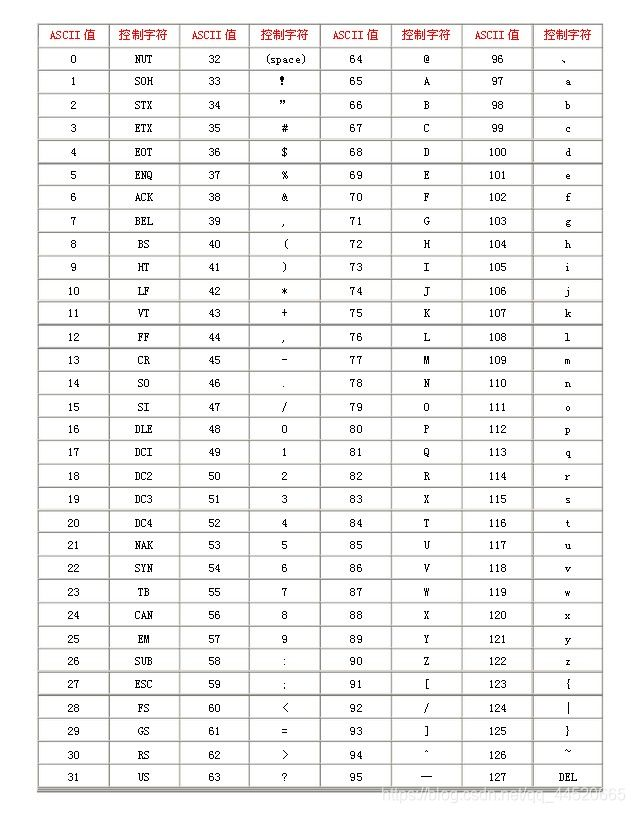
\includegraphics[width=0.9\linewidth]{pic/ascii.jpg}
        \caption{ASCII字符集对应表} \label{ASCII字符集对应表}
    \end{figure}

    \begin{table}[htbp]
        \centering
        \renewcommand\arraystretch{1.5}
        \begin{threeparttable}
            \begin{tabular}{|c|c|} 
                \hline
                ~数据类型~    & ~占用内存(B)~   \\
                \hline \hline
                int         & 4             \\
                \hline
                short       & 2             \\
                \hline
                long        & 4 或 8\tnote{1} \\
                \hline
                char        & 1             \\
                \hline
                float       & 4             \\
                \hline
                double      & 8             \\
                \hline
            \end{tabular} 
            \begin{tablenotes}
                \item[1] 因操作系统而异
            \end{tablenotes}
            \caption{数据类型占用内存表} \label{数据类型占用内存表}
        \end{threeparttable}
    \end{table} 

    \begin{table}[htbp]
        \centering
        \renewcommand\arraystretch{1.5}
        \begin{threeparttable}
            \begin{tabular}{|c|c|}
                \hline
                优先级  & 运算符\tnote{1} \\
                \hline \hline
                1       & \texttt{[]} \ \ \ \texttt{()} \ \ \ \texttt{.} \ \ \ \texttt{->} \\
                \hline
                \multirow{2}{*}{2}       & \texttt{-}$^{\mbox{\scriptsize 负号}}$ \ \ \ \texttt{+}$^{\mbox{\scriptsize 正号}}$ \ \ \ \texttt{(type)} \ \ \ \texttt{++} \ \ \ \texttt{--} \\  
                        & \texttt{*}$^{\mbox{\scriptsize 取值}}$ \ \ \ \texttt{\&}$^{\mbox{\scriptsize 取址}}$ \ \ \ \texttt{!} \ \ \ \texttt{$\sim$} \ \ \ \texttt{sizeof} \\
                \hline
                3       & \texttt{/} \ \ \ \texttt{*}$^{\mbox{\scriptsize 乘法}}$ \ \ \ \texttt{\%} \\
                \hline
                4       & \texttt{+}$^{\mbox{\scriptsize 加法}}$ \ \ \ \texttt{-}$^{\mbox{\scriptsize 减法}}$ \\
                \hline
                5       & \texttt{<<} \ \ \ \texttt{>>} \\
                \hline
                6       & \texttt{<} \ \ \ \texttt{>} \ \ \ \texttt{<=} \ \ \ \texttt{>=} \\
                \hline
                7       & \texttt{==} \ \ \ \texttt{!=} \\
                \hline
                8       & \texttt{\&}$^{\mbox{\scriptsize 按位与}}$ \\
                \hline
                9       & \texttt{\^{}} \\
                \hline
                10      & \texttt{|} \\
                \hline
                11      & \texttt{\&\&} \\
                \hline
                12      & \texttt{||} \\
                \hline
                13      & \texttt{?:} \\
                \hline
                \multirow{2}{*}{14}      & \texttt{=} \ \ \ \texttt{+=} \ \ \ \texttt{-=} \ \ \ \texttt{*=} \ \ \ \texttt{/=} \ \ \ \texttt{\%=} \\
                        & \texttt{<<=} \ \ \ \texttt{>>=} \ \ \ \texttt{\&=} \ \ \ \texttt{\^{}=} \ \ \ \texttt{|=} \\
                \hline
                15      & \texttt{,} \\
                \hline
            \end{tabular}
            \begin{tablenotes}
                \item[1] 表中运算符当发生歧义时运算符后用上标标注运算名称.
            \end{tablenotes}
            \caption{运算符优先级表} \label{运算符优先级表} 
        \end{threeparttable}
    \end{table}
    \chapter{部分较困难问题的解答} \label{部分较困难问题的解答}

    \section{第\ref{循环结构}节问题: } \label{平方和公式答案}
    \begin{enumerate}
        \item 不能.
        \item 因为当\texttt{n}为奇数时, 表达式\texttt{n / 2}因为是整型除以整型, 会发生舍去小数部分, 并不严格等于数学上的$\dfrac{n}{2}$, 从而导致结果错误.
        \item 应当先判断\texttt{n}的奇偶, 根据\texttt{n}的奇偶分别使用: \\
              \texttt{(n + 1) / 2 * n * (2 * n + 1)}~~~~(n为奇数) \\
              \texttt{n / 6 * (n + 1) * (2 * n + 1)}~~~~(n为偶数)
        \item 读者可是试着输入1200, 看看两种方法的输出各是多少. 可以看到第一种发生了意料之外的错误, 而第二种则输出了正确的答案. 这是因为中间的结果其实也是整型, 而在运算过程中产生的中间变量过大, 则可能发生溢出, 发生意料之外的错误. 例如第一种方法由左向右运算, 当计算完第二次乘号时, $1200 \times 1201 \times 2401$已经太大了, \texttt{int}无法支持发生了溢出, 此后再除以6, 也只能得到一个错误的结果. 而第二种方法则先除以了6, 使得中间变量的数值大大减小了, 没有发生溢出, 故输出了正确的结果.
    \end{enumerate}

    \backmatter

    \label{后封面}
\chapter*{\phantom{后封面}}

\emptypage
\ThisCenterWallPaper{1}{pic/cover/backcover.png}
\pagecolor{cover_background_white}
\emptypage

\end{document}

% todo: "pause" check 